\documentclass[pdflatex,11pt]{aghdpl}
% \documentclass{aghdpl}               % przy kompilacji programem latex
% \documentclass[pdflatex,en]{aghdpl}  % praca w języku angielskim
\usepackage[polish]{babel}
\usepackage[utf8]{inputenc}
\usepackage{hyperref} 
\usepackage{amsmath}
\usepackage{verbatim}
\usepackage{graphicx}
\usepackage[toc,page]{appendix}
\hypersetup{%
    pdfborder = {0 0 0}
}

% dodatkowe pakiety
\usepackage{enumerate}
\usepackage{listings}
\lstloadlanguages{TeX}

\lstset{
  literate={ą}{{\k{a}}}1
           {ć}{{\'c}}1
           {ę}{{\k{e}}}1
           {ó}{{\'o}}1
           {ń}{{\'n}}1
           {ł}{{\l{}}}1
           {ś}{{\'s}}1
           {ź}{{\'z}}1
           {ż}{{\.z}}1
           {Ą}{{\k{A}}}1
           {Ć}{{\'C}}1
           {Ę}{{\k{E}}}1
           {Ó}{{\'O}}1
           {Ń}{{\'N}}1
           {Ł}{{\L{}}}1
           {Ś}{{\'S}}1
           {Ź}{{\'Z}}1
           {Ż}{{\.Z}}1
}

%---------------------------------------------------------------------------

\author{Dariusz Mydlarz}
\shortauthor{D. Mydlarz}

\titlePL{
	Możliwości powiązania\linebreak
	danych geolokacyjnych i~analizy sentymentu\linebreak
	w analizie zachowań użytkowników\linebreak
	w wybranych portalach społecznościowych
}
\shorttitlePL{Analiza sentymentu i geolokalizacji w zachowaniach użytkowników portali społeczniościowych}

\thesistypePL{Praca magisterska}
\supervisorPL{dr inż. Anna Zygmunt}
\date{2014}
\facultyPL{Wydział Informatyki, Elektroniki i Telekomunikacji}

\departmentPL{Katedra Informatyki}
\majorPL{Informatyka}

\setlength{\cftsecnumwidth}{10mm}

%---------------------------------------------------------------------------
\begin{document}

\titlepages

\begin{abstract}
Tutaj będzie streszczenie pracy
\end{abstract}
\clearpage
\setcounter{page}{4}
%\setcounter{tocdepth}{1}
\tableofcontents
\clearpage

\listoffigures 
\clearpage
\listoftables
\clearpage
%---------------------------------------------------------------------------
\chapter{Wstęp}
\label{sec:wstęp}
W dzisiejszych czasach wpływ Internetu na życie codzienne jest niepodważalny.
Już od kilku lat świat globalnej wioski przenika się z życiem realnym.
Nikogo nie dziwią już prezentowane w kanałach informacyjnych komentarze
pochodzące z Internetu, których autorami są zarówno osoby znane jak i zwykli
internauci.  Rozrost sieci przebiega w błyskawicznym tempie.
Wydarzenia na świecie komentowane są na żywo przez wielu ludzi -- bez względu na
wiek, płeć czy zawód. Aktualne trendy tworzone są na blogach, mikroblogach czy
serwisach społecznościowych.

Wyzwanie wobec ogromu tych informacji podejmuje dzisiejsza informatyka.
Przetwarzanie tak dużej ilości danych wymaga wielu zautomatyzowanych procesów.
W dzisiejszych czasach nie wystarczy już dowiedzieć się kto z kim najczęściej
się komunikuje, ale dużo bardziej interesujące jest to, o czym dany internauta
pisze i w jaki sposób to czyni.

Wielkie firmy chcą wiedzieć jak odbierane są ich produkty, jakie emocje
wzbudzają wśród klientów ich usługi i czy udaje im się ich zadowolić.
Analiza użytkowników serwisów społecznościowych może być także bardzo
interesującym przedmiotem badań socjologów nad zmieniającym się społeczeństwem i
wpływem Internetu na ten proces.
Dodatkowa analiza geolokalizacji może pozwolić marketingowcom różnych firm na
odkrywanie nowych rejonów świata, w których ich firmy mogłyby oferować swoje
produkty i usługi.

Naprzeciw tym potrzebom budowane są systemy informatyczne, które potrafią takie
informacje uzyskać, przetwarzać i prezentować. Przykład takiego systemu został
zrealizowany w ramach tej\linebreak pracy~magisterskiej.

\section{Cel pracy}
Niniejsza praca skupia się na analizie zachowań użytkowników w wybranych
portalach społecznościowych. Przedmiotem badań są użytkownicy serwisu
mikroblogowego Twitter. W ramach pracy staram się
odpowiedzieć na pytania:
\begin{itemize}
  \item jak internauci korzystają z mediów społecznościowych,
  \item kiedy są najaktywniejsi,
  \item jakie wyrażają emocję,
  \item z jakich miejsc komentują,
  \item czy i w jakie grupy się łączą.
\end{itemize}

Analiza serwisów społecznościowych niesie ze sobą wiele wyzwań. Jako główne można wymienić:
\begin{itemize}
  \item przetwarzanie języka naturalnego -- wiele skrótów, wyrażeń slangowych,
błędów ortograficznych czy typograficznych, sklejanie wyrazów, używanie słów
zapożyczonych z obcych języków, itp.,
  \item ogromna ilość przetwarzanych informacji,
  \item duża liczba krótkich wiadomości,
  \item duża liczba danych zaszumionych -- wpisy reklamowe (SPAM), automatycznie 
wklejanie linków do blogów, innych serwisów społecznościowych, itp.
\end{itemize}

W związku z powyższym zebrane dane muszą być odpowiednio przetworzone i przefiltrowane
zanim zostaną przeprowadzone na nich jakiekolwiek operacje.

W ramach tej pracy pobrałem z serwisu Twitter w ciągu 3 miesięcy blisko 8 milionów
wpisów (w~tym także tych zawierających informacje o geolokalizacji), 
opracowałem metodą analizy sentymentu~-- czyli wydźwięku wypowiedzi (pozytywna,
negatywna lub neutralna) oraz stworzyłem narzędzie wspomagające
analizę zebranych danych -- wyświetlanie szerokiej gamy wykresów, prezentowanie
wpisów na mapie, informowanie o sentymencie -- z możliwością szerokiej selekcji danych do analizy.

\chapter{Przegląd badań}
\label{chapter:przegladbadan}
\begin{comment}
- dużo literatury, przegląd wiedzy dostępnej na dany temat
- sieci społeczne: SNA + analiza zachowań + grupy
- analiza sentymentu: techniki, itd
- twitter
- badania nad geolokacją, zastosowanie, jak
\end{comment}

W niniejszym rozdziale znajduje się aktualny stan badań dotyczący 4 tematów,
które składają się na tę pracę. Na początku opisana jest dziedzina sieci
społecznych, czym ta nauka się zajmuje, w jakich przypadkach może zostać
zastosowana.
Następnie omówiona zostaje analiza sentymentu wypowiedzi i przetwarzanie tekstu
celem ekstrakcji jego wydźwięku.
Później skupiam się nad temat związanym z geolokacją i opisem, co można dzięki
niej się dowiedzieć, a rozdział kończę omówieniem serwisu społecznościowego Twitter,
który został wykorzystany jako źródło danych do analizy sieci społecznych.








% %%%%%%%%%%%%%%%%%%%%%%%%%%%%%%%%%%%%%%%%%%%%%%%%%%%%%%%%%%%%%%% SIECI
% SPOŁECZNE
\section{Sieci społeczne}
Termin ten został użyty po raz pierwszy w 1954 roku przez Johna Arundela Barnesa
\cite{JABarnes}. Oznacza strukturę społeczną, którą tworzą jednostki (np. osoby
lub organizacje) i połączenia między nimi.
Analiza sieci społecznych jest badaną od wielu lat dziedziną nauki. Szybki
rozwój Internetu w XXI wieku wzbogacił ją o bogate źródło danych. Główne obszary
badań \cite{SNDAtopics} to między innymi:
\begin{itemize}
  \item statystyczna analiza sieci społecznych -- opisuje jak wygląda typowa sieć społeczna,
  badane są połączenia między jednostkami, aby sprawdzić czy posiadają kilka połączeń,
  czy sieć zbudowana jest z hubów (osobniki mające dużą liczbę połączeń, 
  łączące ze sobą różne części sieci społecznej; wokół nich koncentrują się inne
  jednostki), czy może liczba połączeń rozłożona jest równomiernie,
  
  \item odkrywanie grup/społeczności -- jest jednym z głównych tematów analizy 
  sieci społecznych; szukanie grup związane jest z klastrowaniem i odkrywaniem 
  obszarów sieci, które są bardziej zagęszczone (czyli takie, w których
  stosunek liczby krawędzi do liczby wierzchołków jest większy niż na zewnątrz);
  problem powiązany jest z badaniem grafów, określaniem jak dzielić sieć na regiony,
  
  \item klasyfikacja wierzchołków -- polega na opracowaniu metody, dzięki której
  możliwe jest zaklasyfikowanie wierzchołków do wcześniej zdefiniowanych klas na
  podstawie podobieństwa z innymi jednostkami do tych klas już należących,
  
  \item odnajdywanie ekspertów -- sieci społeczne mogą być używane jako narzędzia
  w celu odkrywania ekspertów do danego zadania,
  
  \item predykcja przyszłych połączeń wewnątrz sieci -- wiele badań skupia
  się na statycznych połączeniach wierzchołków; w wielu sieciach jednak 
  połączenia między węzłami są dynamiczne i badania te koncentrują się na 
  tym by przewidzieć nowe połączenia wewnątrz sieci,
  
  \item ekstrakcja wiedzy z sieci -- polega na eksploracji danych z mediów 
  społecznościowych i eksploracji tekstu z serwisów społecznościowych; 
  eksploracja danych dostarcza naukowcom narzędzia do analizy dużych, 
  złożonych i często zmieniających się danych wewnątrz sieci, a eksploracja tekstu
  może prowadzić do odkrycia nowych połączeń między węzłami i nowych
  charakterystyk je łączących; jej użycie wpływa na poprawę jakości
  badanej sieci. 
\end{itemize}



\subsection{Przykłady zastosowania sieci społecznych}
Wyniki badań nad sieciami społecznymi stwarzają wiele możliwości dla różnych
dziedzin życia. Mogą być zastosowane między innymi przez:
\begin{itemize}
  \item służby porządkowe -- policja może przy ich pomocy odkrywać powiązania
  między przestępcami i dochodzić do zależności między grupami przestępczymi,
  a także odkrywać, kogo dane grupy mogłyby zwerbować, 
  \item badania naukowe -- odkrywanie naukowców zajmujących się podobnymi tematami
  celem opracowania bardziej kompletnych wyników lub podjęcia nowego,
  wspólnego tematu,
  \item przedsiębiorstwa handlowe -- odkrywanie zbliżonych typów klientów i 
  oferwanie im produktów lub usług do nabycia przy użyciu systemów rekomendujących,
  \item służby zdrowotne -- użycie sieci społecznych może pomóc w określaniu
  obszarów, w które rozprzestrzeniają się wirusy gróźnych chorób, dzięki czemu
  możliwe może być zapobieganie ich dalszej ekspansji.
\end{itemize}



\subsection{Reprezentacja sieci społecznych}
Najczęściej spotykaną reprezentacją sieci społecznych jest reprezentacja
grafowa. Grafem nazywamy strukturę G = (V, E) składającą się z węzłów
(wierzchołków, oznaczonach przez V) wzajemnie połączonych za pomocą krawędzi
(oznaczanych przez E). Przykładowy graf został zaprezentowany na rysunku
\ref{image:graf-zwykly}.

\begin{figure}[ht!]
\centering
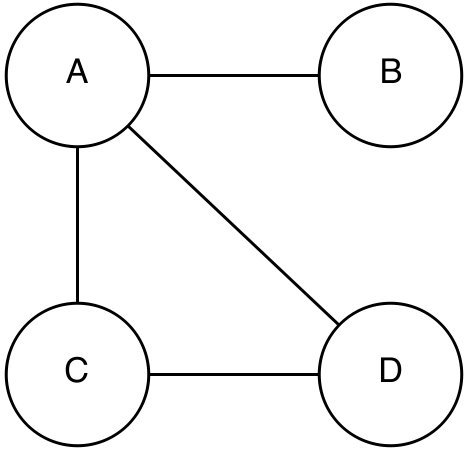
\includegraphics[width=40mm]{img/graf-zwykly.png}
\caption{Graf o 4 wierzchołkach i 4 krawędziach}
\label{image:graf-zwykly}
\end{figure}

Reprezentacja grafowa w naturalny sposób modeluje jednostki jako węzły i relacje
między nimi jako krawędzie. W zależności od rodzaju sieci graf taki może
posiadać krawędzie skierowane lub nieskierowane oraz ważone lub nieważone.
Krawędź skierowana reprezentuje kierunek, w którym przebiega komunikacja między
węzłami. Krawędź ważona może reprezentować  liczbę wiadomości wymienionych
między węzłami lub jakiś inny rodzaj wagi (oznaczania jednych krawędzi
za bardziej istotne od innych). Przykładowy graf skierowany o krawędziach ważonych
przedstawia rysunek \ref{image:graf-skierowany}.

\begin{figure}[ht!]
\centering
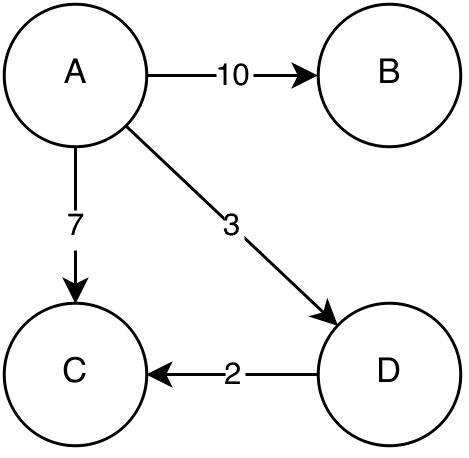
\includegraphics[width=40mm]{img/graf-skierowany.png}
\caption{Graf skierowany o krawędziach ważonych}
\label{image:graf-skierowany}
\end{figure}
















%%%%%%%%%%%%%%%%%%%%%%%%%%%%%%%%%%%%%%%%%%%%%%%%%%%%%% MIARY I POJĘCIA GRAFOWE

\subsection{Miary i pojęcia grafowe}
Zamodelowanie sieci społecznych w postaci grafów pozwala na skorzystanie z szeregu
miar związanych z tą dziedziną wiedzy. Dzięki nim możliwe jest odnajdywanie cech
charakterystycznych danej sieci. Najważniejsze miary pomagające odnaleźć najważniejsze
węzły to \cite{estrada}: 


\subsubsection{Stopień wierzchołka}
Miara określająca liczbę krawędzi wchodzących i 
  wychodzących z wierzchołka (patrz rys. \ref{image:stopien-wierzcholka})
  
\begin{figure}[ht!]
\centering
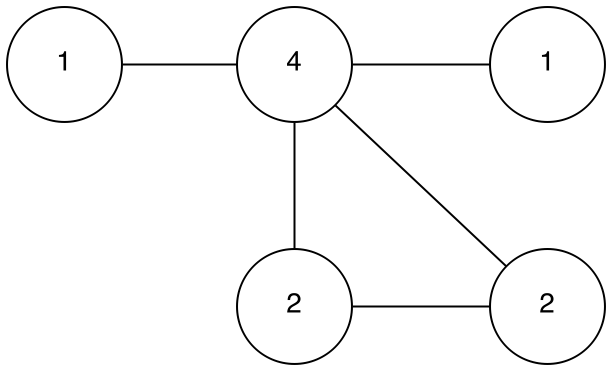
\includegraphics[width=80mm]{img/stopien-wierzcholka.png}
\caption{Graf z oznaczonymi stopniami wierzchołków}
\label{image:stopien-wierzcholka}
\end{figure}

W przypadku grafów skierowanych możemy jeszcze mówić o stopniu wchodzącym 
(ang. \textit{in degree}) oraz wychodzącym (ang. \textit{out degree}) 
(patrz rys. \ref{image:stopien-wierzcholka-skierowany}).
  
\clearpage
\begin{figure}[ht!]
\centering
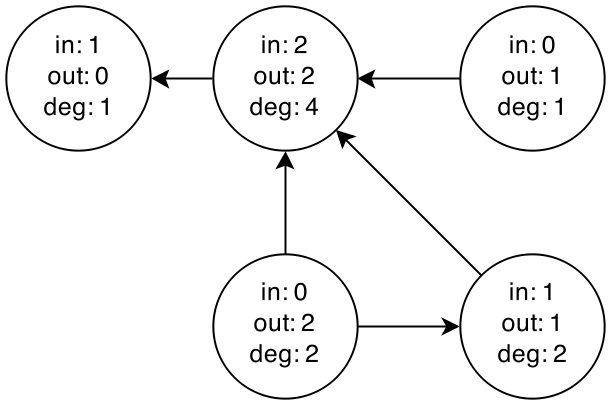
\includegraphics[width=80mm]{img/stopien-wierzcholka-skierowany.png}
\caption{Graf skierowany z oznaczonymi stopniami wierzchołków}
\label{image:stopien-wierzcholka-skierowany}
\end{figure}
  
  
\subsubsection{Pośrednictwo (ang. \textit{betweenness}) }  
Liczba najkrótszych ścieżek w grafie, które przechodzą przez dany węzeł podzielona
przez liczbę wszystkich najkrótszych ścieżek grafu. Przez najkrótszą ścieżkę 
rozumie się taką ścieżkę między dwoma węzłami grafu, dla której liczba krawędzi
jest najmniejsza.
  
\begin{equation}
BC(k) = \sum\limits_{i}\sum\limits_{j}\frac{\rho(i, k, j)}{\rho(i, j)}, \quad i \neq j \neq k
\end{equation}

gdzie:

$\rho(i, k, j)$ -- liczba najkrótszych ścieżek pomiędzy $i$ oraz $j$ przechodząca
przez wierzchołek $k$,

$\rho(i, j)$ -- liczba wszystkich najkrótszych ścieżek pomiędzy $i$ oraz $j$.

\bigskip

Przykładowo aby obliczyć wartość tej miary dla wierzchołka $B$ posłużmy się rysunkiem 
\ref{image:betweenness}.
Najkrótsze ścieżki między węzłami innymi niż $B$ to: $ABC,$ $ABD$, $ABE$, $CBD$, $CBE$, $DE$.
\mbox{W 5 z 6 z nich} znajduje się węzeł $B$, stąd wynika jego wartość \textit{betweenness}
równa $5/6$. 

\begin{figure}[ht!]
\centering
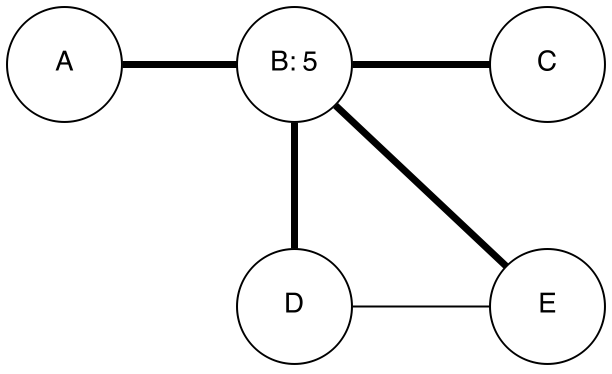
\includegraphics[width=80mm]{img/betweenness.png}
\caption{Najkrótsze scieżki przechodzące przez węzeł $B$}
\label{image:betweenness}
\end{figure}

Węzły o wysokiej wartości współczynnika \textit{betweenness} są interesujące
ponieważ mogą kontrolować przepływać informacji wewnątrz sieci oraz
mogą być zmuszone do przetwarzania większej ilości informacji.
Z tego wynika też, że mogą być skutecznym celem ataków.
    
  
\clearpage  
\subsubsection{Bliskość (ang. \textit{closeness})}  
Znormalizowana odwrotność sumy odległości między węzłami w grafie.
  
\begin{equation}
CC(k) = \frac{\sum\limits_{j}d(k, j)}{N - 1}
\end{equation}  

gdzie:

$d(k, j)$ -- odległość między wierzchołkami $k$ oraz $j$,

$N$ -- liczba wszystkich wierzchołków.

\bigskip

Wartość \textit{closeness} dla pojedynczego wierzchołka liczymy sumując
odległości między nim a pozostałymi wierzchołkami,
a następnie dzielimy tę wartość przez $N - 1$. Przykładowy graf \ref{image:closeness} i tabela 
\ref{tab:closeness} z obliczeniami tej wielkości znajdują się poniżej.


\begin{figure}[ht!]
\centering
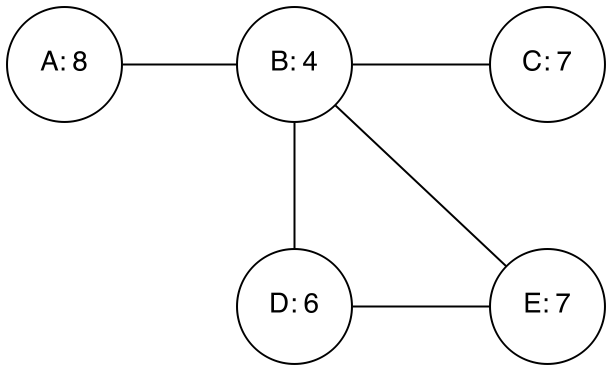
\includegraphics[width=80mm]{img/closeness.png}
\caption{Suma odległości do pozostałych węzłów w grafie}
\label{image:closeness}
\end{figure}
  

\begin{table}[ht!]  
\begin{center}  
\begin{tabular}{| c | c c c c c || c | c |}
 \hline
 & \multicolumn{5}{c ||}{Wierzchołki} & Suma odległości & Bliskość (\textit{closeness}) \\
 \hline
 & A & B & C & D & E &  $S = \sum\limits_{j}d(i, j)$ & $CC(i) = \frac{S}{N - 1} = \frac{S}{4}$ \\
\hline
A & 0 & 1 & 2 & 2 & 3 & 8 & 0.5 \\ 
B & 1 & 0 & 1 & 1 & 1 & 4 & \textbf{1.0} \\ 
C & 2 & 1 & 0 & 2 & 2 & 7 & 0.57 \\ 
D & 2 & 1 & 2 & 0 & 1 & 6 & 0.67 \\ 
E & 3 & 1 & 2 & 1 & 0 & 7 & 0.57 \\ 
 \hline
\end{tabular} 
\end{center} 
\caption{Odległości między węzłami i wartości miary \textit{closeness}}
\label{tab:closeness}
\end{table}
  
Węzłem o najmniejszej sumie odległości do innych wierzchołków -- a co za tym idzie --
o największej wartości bliskości jest węzeł $B$. Wynika z tego, że jest to
wierzchołek najszybciej rozsyłający informacje wewnątrz sieci pomiędzy jej elementami. 


\clearpage
\subsubsection{Wektor własny (ang. \textit{eigenvector})}
Miara centralności węzła,  która oceniając dany węzeł bierze także pod uwagę 
wartości jego sąsiadów (bezpośrednio przyległych węzłów).
Zastosowanie tej wielkości pozwala wskazać najważniejszy węzeł w sytuacji,
gdy poprzednie miary zwracają równe wyniki. Wartość tej wielkości wyraża się
wzorem:

\begin{equation}
EV(k) = \frac{1}{\lambda}\sum\limits_{j}A_{kj}x_j
\end{equation}

gdzie:

$\lambda$ -- stała, równa największej wartości własnej macierzy sąsiedztwa grafu,

\begin{math}
 A_{kj} =
  \begin{cases}
   1, \text{gdy wierzchołki $k$ oraz $j$ mają wspólną krawędź} \\
   0, \text{w przeciwnym wypadku}
  \end{cases}

\end{math}


\bigskip

Przykładowe wartości wielkości \textit{eigenvector}
zaprezentowano na rysunku \ref{image:eigenvector}. Wartości te zostały
obliczone przy pomocy narzędzia Gephi\footnote{https://gephi.github.io/}.

\begin{figure}[ht!]
\centering
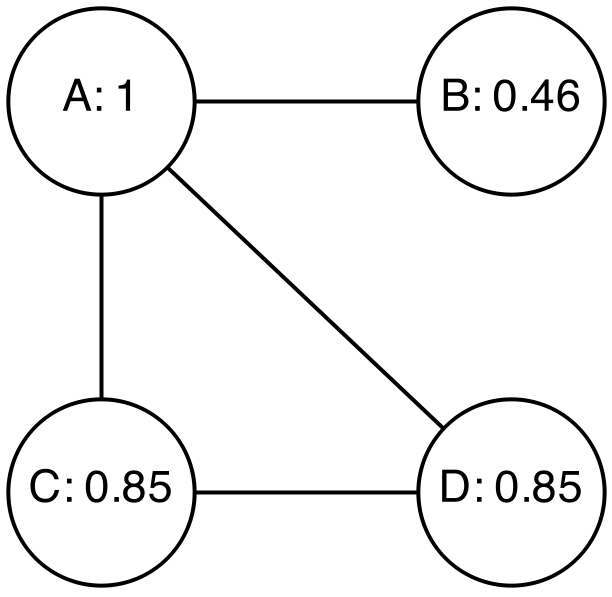
\includegraphics[width=40mm]{img/eigenvector.png}
\caption{Wartości wielkości \textit{eigenvector} w przykładowym grafie}
\label{image:eigenvector}
\end{figure}


\subsubsection{Klika}
W analizie sieci społecznych (traktowanych jako graf) przydatne są także 
2 następujące pojęcia:
\begin{itemize}
  \item klika -- podgraf grafu, w którym wszystkie wierzchołki połączone są 
  krawędzią,
  \item k-klika -- klika składająca się z dokładnie $k$-wierzchołków. Na przykład
  k-klika o $k=3$ to podgraf zbudowany z 3 wierzchołków, gdzie między każdym z 
  nich znajduje się krawędź (patrz rys. \ref{image:klika}).
\end{itemize}

\clearpage
\begin{figure}[ht!]
\centering
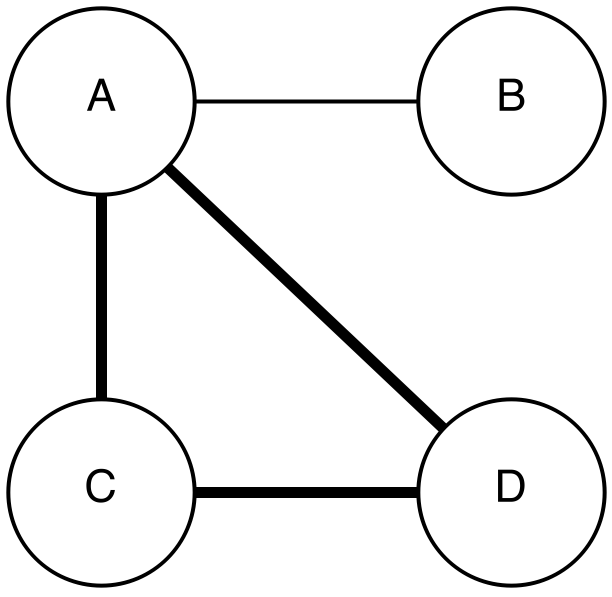
\includegraphics[width=40mm]{img/klika.png}
\caption{K-klika o rozmiarze 3 zbudowana przez wierzchołki $ACD$}
\label{image:klika}
\end{figure}








% %%%%%%%%%%%%%%%%%%%%%%%%%%%%%%%%%%%%%%%%%%%%%%%%%%%%%%%%%%%%%%%%%%%%%
% SENTYMENT
\section{Sentyment wypowiedzi}
Sentyment (inaczej wydźwięk wypowiedzi) to stosunek lub postawa wobec jakiejś
sytuacji, zdarzenia. Badanie sentymentu niesie ze sobą bardzo dużo informacji.
Recenzje, komentarze i opinie odgrywają istotną rolę w ocenie satysfakcji z
produktu lub usługi czy w badaniu reakcji na wydarzenia. Dane, które zawierają
takie informacje mają bardzo wysoki potencjał w odkrywaniu wiedzy.
Dowiadywanie się, co myślą inni ludzie zawsze było bardzo istotne w procesie
podejmowania decyzji. Internet daje możliwość zapoznania się z opiniami innych
ludzi czy ekspertów. Możliwość analizy sentymentu wypowiedzi może być bardzo
pomocna. Jak wynika z badań przeprowadzonych na ponad 2000 dorosłych Amerykanów
\cite{pangLee} 81\% użytkowników Internetu przynajmniej raz poszukiwało w
Internecie informacji o jakimś produkcie z czego od 73\% do 87\% osób twierdzi,
że recenzje innych miały wpływ na ich wybory.

Zastosowanie analizy sentymentu jest bardzo szerokie. Niektóre
z obszarów jej użycia to \cite{pangLeeApplication}:
\begin{itemize}
  \item portale internetowe z opiniami -- zastosowanie analizy sentymentu
może być użyte do poprawy błędów popełnionych przez użytkowników (gdy opinia
jest pozytywna, a użytkownik omyłkowo wybrał niską ocenę) lub gdy opinie
są ewidentnie stronnicze, mogą pomóc w faktycznej ocenie danego przedmiotu czy 
usługi
\item jako technologia wspomagająca większe systemy -- analiza sentymentu może
być wsparciem dla systemów rekomendacji; na przykład może służyć do 
tego by nie rekomendować produktów, które otrzymały negatywne opinie; 
w systemach serwujących reklamy kontekstowe, wykrycie pozytywnego sentymentu
na stronie może być powodem wyświetlenia jakiejś reklamy,
a wykrycie negatywnego sentymentu powodem jej ukrycia;
innym zastosowaniem jest ekstrakcja informacji, która może być
polepszona poprzez pomijanie zdań subiektywnych, zawierających sentyment
\item biznes -- poprzez dostarczenie informacji o odbiorze sprzedawanych produktów
i serwowanych usług; gdy na przykład sprzedawany laptop ma negatywny odbiór
stosując analizę sentymentu można to bardzo szybko wykryć i dowiedzieć się
dlaczego zaistniała dana sytuacja; firma może badać swój ogólny odbiór
w społeczeństwie -- szybko reagować na niezadowolenie klientów, lub wprowadzać
poprawki do swoich produktów; wykrywanie sentymentu może również pomóc
przewidzieć wyniki sprzedaży
\item polityka -- użycie analizy sentymentu jest wręcz naturalne dla tego obszaru
życia; partie czy politycy mogą badać odbiór społeczeństwa swoich programów
i decyzji; badanie sentymentu może im na przykład wskazać w jakich miejscach,
czy przy jakich postaciach się pokazać by zyskać sympatię wyborców; istotne
również mogą być informacje na temat reakcji społeczeństwa na planowane
przez rząd zmiany w prawie. 
\end{itemize}

Krótko mówiąc największym zyskiem związanym z badaniem sentymentu jest możliwość
zbadania opinii bardzo dużej liczby osób w sposób mechaniczny. Nie ma potrzeby
przeprowadzania ankiet, pytania ludzi co sądzą na dany temat. Internauci samodzielnie
przedstawiają swoje opinie w Internecie, a przy pomocy analizy sentymentu bardzo
łatwe staje się zbadanie nastrojów.



Badanie sentymentu nie jest trywialne. Związane jest bezpośrednio z 
przetwarzaniem języka naturalnego, które niesie ze sobą szereg problemów:

\begin{itemize}
  \item złożoność języka naturalnego -- bardzo trudnym zadaniem jest nauczenie 
programu komputerowego pełnego rozumienia języka naturalnego; co więcej każdy
język jest inny, więc dla każdego konieczne jest zastosowanie różnych
rozwiązań -- inaczej trzeba podejść do badania sentymentu w języku polskim
a inaczej w angielskim; trzeba pamiętać też, że język naturalny nie jest martwy 
i ciągle się rozwija,
\item trudność w analizie kontekstu wypowiedzi -- wykrycie ironii nie jest zadaniem 
prostym; bardzo często wypowiedzi mogą mieć związek z jakimś pojęciem 
zupełnie niezrozumiałym dla programu komputerowego, a oczywistym dla człowieka
(np. idiomy, odniesienia do wydarzeń na świecie)
\item slang w Internecie, skrótowce, literówki -- wszystkie te elementy
dodatkowo utrudniają analizę sentymentu; użytkownicy Internetu nie zawsze
dbają o jakość swojego języka, często stosują skróty, czy wyrażenia slangowe, 
które mogą być niezrozumiałe dla automatycznego analizatora sentymentu;
\item SPAM, szum -- wszystkie wpisy, które nie niosą ze sobą żadnej wartości
a pojawiają się w internetowych forach, serwisach z opiniami również stanowią
wyzwanie przy budowie narzędzia do analizy sentymentu.
\end{itemize}


\subsection{Techniki badania sentymentu}
Podejść do badania sentymentu jest wiele. Poniżej przedstawione są te, które
najlepiej nadają się do badania sentymentu na Twitterze (w związku z tym, że to
ten serwis jest źródłem danych w tej pracy), a które zostały opisane w artykule 
\cite{sentimentTechniques}. Oprócz nich przedstawię także metodę opracowaną
przez Alexandra Paka i Patricka Paroubek'a \cite{pakParoubekSentiment}, którą 
zastosowałem w swoich badanich. Techniki te to:

\subsubsection{Podejście oparte na słowniku (ang. \textit{lexicon based approach})}
Podejście polega na zastosowaniu słownika z wyrazami oznaczonymi jako pozytywne
i negatywne. Klasyfikator ocenia tekst na podstawie liczby wystąpień
odpowiednich słów. Niestety podejście to ma bardzo wysoki stopień błędów.
Przykładowa funkcja oceniająca sentyment słowa to:
\begin{equation}
X_t = \frac{P(pos | topic, t)}{P(neg | topic, t)}
\end{equation}

gdzie:

$P(pos | topic, t)$ -- prawdopodobieństwo zdarzenia, że słowo $t$ w temacie 
$topic$ wystąpi z sentymentem pozytywnym,

$P(neg | topic, t)$ -- prawdopodobieństwo zdarzenia, że słowo $t$ w temacie
$topic$ wystąpi z sentymentem negatywnym.

\bigskip


W tym przypadku wyrazy mają przypisany odpowiedni sentyment w zależności od
tematu, którego dotyczą. Największym problemem tego podejścia jest brak
mechanizmu radzenia sobie z kontekstem słów.

\subsubsection{Naiwny klasyfikator Bayesa (ang. \textit{naive Bayes classifier})}
Jest to podejście probabilistyczne. W ramach tej metody zakłada się, że dana kategoria
tekstów $k_1$ (np. pozytywne) charakteryzuje się określonym słownictwem, 
a inna $k_2$ (negatywne) innym słownictwem. 
Na tej podstawie określamy prawdopodobieństwo jeszcze przed przeprowadzeniem
jakiejkolwiek klasyfikacji tekstu. Zakłada się także, że tekst, który posiada
słownictwo z kategorii $k_1$ w większej liczbie niż z kategorii $k_2$, powinien
być zaklasyfikowany do tej pierwszej. 
W tym przypadku jest to określenie klasyfikacji posiadając pewną wiedzę na temat
badanego tekstu.

Naiwny klasyfikator Bayesa opiera się na założeniu o wzajemnej niezależności
słów. Oznacza to, że wyrazy, które identyfikują określoną kategorię mogą występować
niezależnie w różnych lub tym samym tekście. Taki naiwny klasyfikator może więc 
identyfikować i klasyfikować słowa, nie biorąc pod uwagę kontekstu w jakim one
występują. Pomimo, że jest to podejście naiwne, okazuje się skuteczne ze względu
na swoją prostotę. Wzór Bayesa określa bowiem prawdopodobieństwo tego, że szanse
przypisania tekstu do odpowiedniej klasy zależą od tego jak często jego słowa
należą do różnych klas i jak często do nich nie należą.

Krótko mówiąc, jeśli naiwny klasyfikator Bayesa w wybranym tekście znajdzie więcej
słów należących do klasy pozytywnej i jednocześnie mniej należących do negatywnej,
wówczas większe będzie prawdopodobieństwo zaklasyfikowania tekstu do pierwszej
kategorii. Klasyfikator ten uczy się klas wyrazów sukcesywnie analizując
kolejne teksty \cite{tomanekSentyment}.



\subsubsection{Technika maksymalnej entropii (ang. \textit{maximum entropy technique})}
Technika estymacji rozkładu prawdopodobieństwa. Główna zasada polega na tym,
że jeśli dane nie są dobrze znane, rozkład powinien być jak najbardziej jednolity,
to znaczy mieć maksymalną entropię. Do tej techniki mogą dochodzić ograniczenia,
które pozwalają by rozkład nie był maksymalnie jednolity. Ograniczenia
takie mogą pochodzić z oznaczonych już danych treningów i reprezentowane jako
oczekiwane wartości wybranych cech (wyrazów). 

Na przykład w jakimś przypadku
możemy założyć, że 50\% wpisów jest pozytywnych, wówczas pozostałe klasy
powinny posiadać po 25\% prawdopodobieństwa (negatywne, neutralne).
Taki model jest łatwy do zbudowania, ale staje się on bardziej skomplikowany
wraz z rosnącą liczbą ograniczeń. Jako cechy dodawane mogą być również
składniki wielowyrazowe zwiększające skuteczność tej techniki. Dlatego też
podejście to nie cierpi z powodu założenia o niezależności wyrazów.
Przykładowo wyrażenie ,,do widzenia'' może być traktowane jako całościowy term,
a nie jako każdy wyraz z osobna.

Niestety w związku z tym, że ograniczenia pochodzą z danych treningowych,
jest duża szansa, że dane te będą relatywnie rzadkie i metoda ta może prowadzić
do przeuczenia.


\subsubsection{Metoda wektorów nośnych (ang. \textit{support vector machines})}
Support vector machines to podejście stosujące duży margines między klasami.
Główna idea polega na znalezieniu hiperpłaszczyzny, która podzieli teksty na pozytywne
i negatywne z marginesem pomiędzy klasami tak dużym jak to tylko możliwe.
Technika ta zbudowana jest na zasadzie strukturalnej minimalizacji ryzyka 
(ang. \textit{structural risk minimization principle}). Celem jest znalezienie
funkcji $h$, dla której błąd klasyfikacji losowego tekstu będzie jak najmniejszy.
Można ją opisać wzorem:
\begin{equation}
\vec{h} = \sum\limits_{i}\alpha_iC_i\vec{t_j}, \quad \alpha_i \geq 0
\end{equation}

gdzie:

$\vec{h}$ -- szukana hiperpłaszczyzna,

$\vec{t_j}$ -- badany tekst (pojedynczy wpis),

$C_j \in \{1, -1\}$ -- klasy, do których może trafić wpis (pozytywna/negatywna),

$\alpha_i$ -- wartość, która może być znaleziona przez rozwiązanie problemu
podwójnej optymalizacji.

\bigskip

Teksty o $\alpha_i$ większym od zera, to te które biorą udział
w szukaniu funkcji $h$ i nazywa się je wektorami wspierającymi 
(ang. \textit{support vectors}).

Wybór cech (wyrazów) jest bardzo ważnym zadaniem w technikach uczenia maszynowego.
Musi to zostać tak wykonane by uniknąć przeuczenia i jednocześnie zwiększyć
ogólną dokładność. Maszyny wektorów nośnych mają wysoki potencjał radzenia
sobie z dużą liczbą wymiarów. Mierzą złożoność hipotezy którą dzielą dokumenty, 
a nie liczbę cech. W związku z tym liczba cech nie jest problemem.
Technika ta radzi sobie z duża liczbą słów poprzez oznaczanie części z nich jako
nieistotne (tych najrzadziej pojawiających się). Niestety czasami prowadzi to 
do utraty informacji. 

Chociaż SVM przewyższa wszystkie tradycyjne metody klasyfikacji sentymentu,
to niestety jest czarną skrzynką. Trudne jest zbadanie natury klasyfikacji i
zidentyfikowanie, które słowa są dla niej istotne. Jest to jedna z głównych wad
korzystania z tej techniki do klasyfikacji tekstów. 

\subsubsection{Metoda Alexandra Paka i Patricka Paroubek'a}
\label{subsubsection:pakandparoubek}
Technika jest odpowiedzią na problemy związane z brakiem odpowiedniego słownika
do oceny sentymentu. Została opracowana z uwzględnieniem Twittera i korzysta
w związku z tym z pewnych założeń. Skoro nie ma żadnego idealnego słownika
ze słowami oznaczonymi jako pozytywne lub negatywne, to trzeba go mechanicznie
zbudować. Do budowy takiego leksykonu zostały wykorzystane wpisy na Twitterze,
które zawierają emotikony podzielone na pozytywne (np. \texttt{:)}) i 
negatywne (np. \texttt{;(}). 

Następnie spośród ściągniętych wpisów z Twittera analizowane są te,
które zawierają odpowiednie emotikony i zliczana jest liczba wystąpień
każdego wyrazu w każdym ze zbiorów (pozytywnym i negatywnym).
W wyniku tego budowany jest leksykon zawierający wyrazy wraz z liczbą
ich wystąpień w każdej z klas.
W związku z tym, że wpisy na Twitterze ograniczone są do 140 znaków, autorzy przyjęli
założenie, że emotikona dotyczy całego wpisu. 
Ocena tekstu $T$ składającego się z wyrazów obliczana jest jako:

\begin{equation}
valence(T) = \frac{\sum\limits_{i = 1}^n valence(w_i)}{n}
\label{equation:pakparoubek}
\end{equation}

gdzie:

$T$ -- tekst poddany analizie,

$w_i$ -- pojedyncze słowo w tekście $T$,

$valence(w_i)$ -- wartość $valence$ dla słowa $w_i$,

$n$ -- liczba słów w tekście $T$.

\bigskip


Wartość $valence(w_i)$ obliczana jest przy zastosowaniu skonstruowanego
leksykonu i równa delta IDF (ang. \textit{inverse document frequency} -- 
powszechnie stosowana miara ważności słowa w oparciu o liczbę wystąpień):
\begin{equation}
valence(w_i) = log\frac{N(w_i, M^+) + 1}{N(w_i, M^-) + 1}
\end{equation} 

gdzie:

$N(w_i, M^+)$ -- liczba wystąpień słowa $w_i$ w zbudowanym leksykonie w 
kontekście pozytywnym,

$N(w_i, M^-)$ -- liczba wystąpień słowa $w_i$ w zbudowanym leksykonie w 
kontekście negatywnym.

\bigskip
Zastosowanie takiego wzoru prowadzi do tego, że niezależnie jak często
dany wyraz pojawia się w zbiorze treningowym, najważniejsza jest jego polaryzacja.
Gdy na przykład słowo \textit{świetny} pojawia się w zbiorach pozytywnym
i negatywnym odpowiednio 1000 i 20 razy, a słowo \textit{przezacny} odpowiednio
50 i 1 raz to ich wpływ na ocenę tekstu będzie identyczny.


\subsubsection{Ocena pozytywności wpisu * do koncepcji}
W kilku miejscach została zastosowana miara pozytywności wpisu.
Została ona wyliczona przy pomocy następującego równania:

\begin{equation}
\label{equation:pozytywnosc}
P = \frac{|pos|}{|pos| + |neg|}
\end{equation}

gdzie:

$|pos|$ -- liczba wpisów oznaczonych jako pozytywne,

$|neg|$ -- liczba wpisów oznaczonych jako negatywne.










%%%%%%%%%%%%%%%%%%%%%%%%%%%%%%%%%%%%%%%%%%%%%%%%%%%%%%%%%%%%%%%%%%%%%% GEOLOKACJA
\clearpage\section{Geolokacja}
Geolokacja to sposób, technika identyfikacja geograficznego położenia osoby
lub urządzenia za pomocą cyfrowych narzędzi przetwarzanych w 
Internecie\footnote{Oxford Dictionaries -- www.oxforddictionaries.com}.

Główne sposoby pozyskiwania takich danych to:
\begin{itemize}
  \item korzystanie z urządzeń GPS -- wbudowanych we współczesne telefony
komórkowe, tablety, itp.,
  \item pozycjonowanie względne -- ustalanie pozycji na podstawie bazowych stacji
telefonii komorków, ruterów WI-FI,
\item użcyie bazy adresów przypisanych do IP.
\end{itemize} 
Zastosowanie geolokacji może być bardzo szerokie, między innymi:
\begin{itemize}
  \item dostarczanie lokalnych wiadomości
  \item dystrybucja treści cyfrowych -- może być np. blokowana możliwość kupna, 
  dla niektórych lokalizacji
  \item wyszukiwanie lokalnych usług, przedsiębiorstw
  \item wyświetlanie zlokalizowanych reklam
  \item zapobieganie nadużyciom zakupowym -- sprawdzenie geolokacji
  klienta sklepu internetowego i porównanie jej z danymi z karty kredytowej,
  w celu ochrony osób, którym na przykład taka karta została skradziona
  \item prezentowanie różnych treści na stronach w zależności od lokalnego
  prawego (np. ukrywanie treści zabronionych w danym miejscu).
\end{itemize}
W szczególności w przypadku sieci społecznych geolokacja może być pomocna do
ustalenia miejsca przebywania danych grup i może prowadzić
do uzupełnienia zebranych danych o kolejne, wzbogacające analizę danej społeczności,
pozwalające na wyciągnięcie bogatszych wniosków. Pomocnym może być na przykład
zbadanie reakcji społeczeństwa w różnych regionach kraju na planowane zmiany
w prawie przez rząd -- i może to prowadzić albo do ich wprowadzenia albo wycofania.

Jako główne zalety stosowania geolokacji \cite{lostInGeolocation} z punktu
widzenia użytkowników telefonów komórkowych i sieci społecznych wymienia się
dzielenie się ze społecznością (56\%) oraz dzielenie się z osobami, które się 
zna lub można poznać (spotkać) (41\%). Głównymi problemami związanymi z 
dzieleniem się geolokacją są obawy o prywatność (33\%) oraz brak korzyści z niej
wynikających (26\%).



%%%%%%%%%%%%%%%%%%%%%%%%%%%%%%%%%%%%%%%%%%%%%%%%%%%%%%%%%%%%%%%%%%%%%% TWITTER
\clearpage\section{Twitter}
Twitter\footnote{www.twitter.com} to serwis społecznościowy o charakterystyce mikrobloga zorientowany
na szybką i bezpośrednią komunikację. Pozwala on
na umieszczanie wpisów nie dłuższych niż 140 znaków. Domyślnie wszystkie 
wpisy są publiczne, a użytkownicy mają możliwość publicznej wymiany zdań
z innymi. Każdy użytkownik ma możliwość wyboru użytkowników, których
wpisy chce widzieć na swojej stronie głównej.

Podstawowe pojęcia związane z tym serwisem to (oznaczone na rysunku \ref{image:twitter-screen}):

\begin{figure}[ht!]
\centering
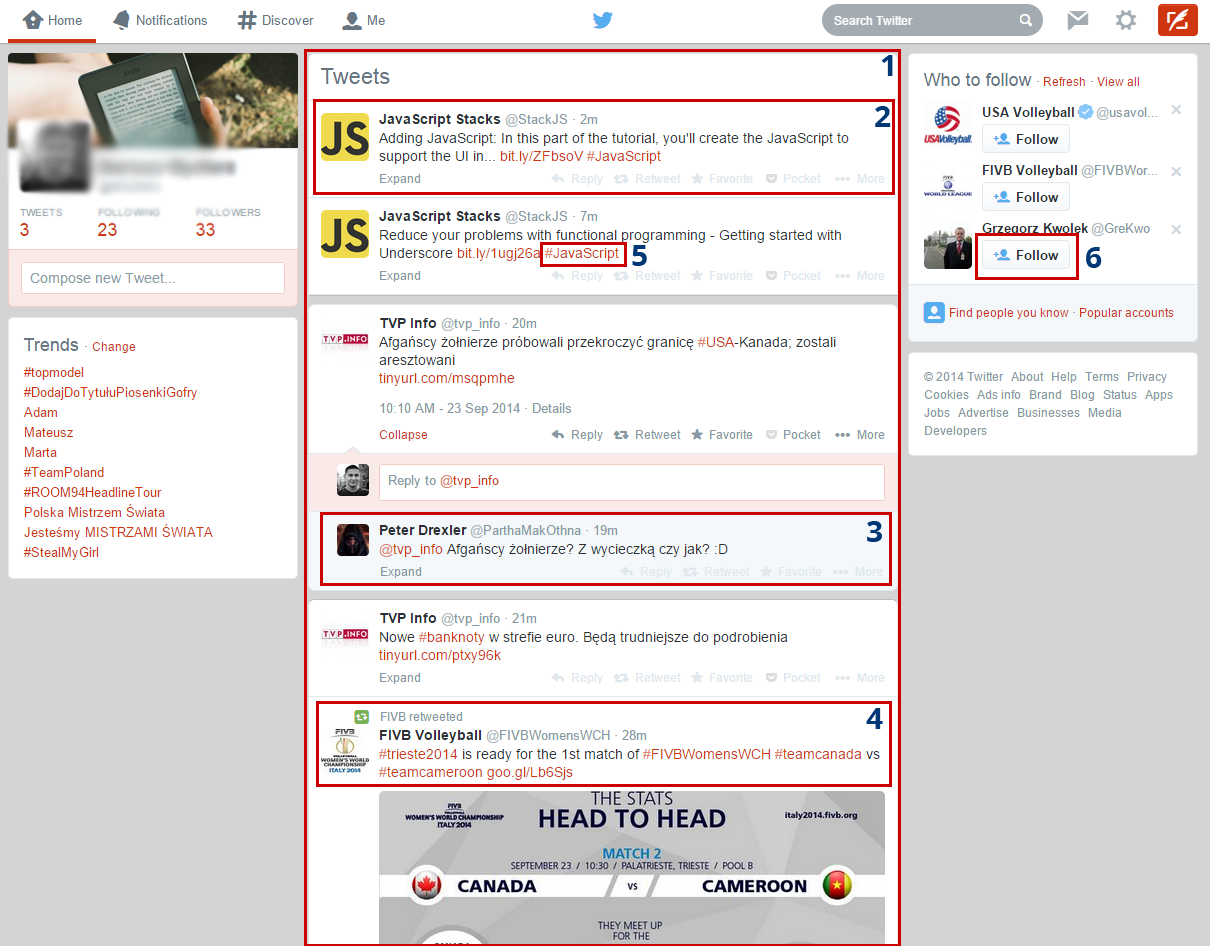
\includegraphics[width=160mm]{img/twitter-screen2.png}
\caption{Budowa serwisu Twitter}
\label{image:twitter-screen}
\end{figure}

\begin{enumerate}
  \item Ściana wpisów (ang. \textit{newsfeed}) -- inaczej strona główna 
  użytkownika, na której widzi wszystkie tweety wysłane przez osoby, które śledzi.
  
  \item Wpis (ang. \textit{tweet}) -- pojedynczy wpis/post na Twitterze; 
  maksymalna długość to 140 znaków; może dodatkowo zawierać zdjęcie lub 
  informację o geolokalizacji.

  \item Odpowiedź (ang. \textit{reply}) -- odpisanie na jakąś wiadomość w serwisie
  Twitter, skomentowanie jej; serwis łączy takie wpisy w jedną grupę, wyświetlając
  je jeden obok drugiego.
  
  \item Podanie wpisu dalej (ang. \textit{retweet}) -- oznacza przekazanie 
  jakiegoś wpisu dalej; jeśli użytkownik A użyje funkcji
  retweet dla dowolnego wpisu w serwisie, wówczas osoby śledzące użytkownika A, 
  również zobaczą ten wpis na swojej stronie głównej.
  
  \item Wyraz z symbolem kratki (ang. \textit{hashtag}) -- użycie symbolu \# 
  wraz z jakimś słowem; ułatwia rozmowy na wspólne tematy, wśród większych grup
  użytkowników (np. \textit{\#worldcupfinal} dla osób komentujących finał 
  mistrzostw świata).

  \item Śledzenie (ang. \textit{follow}) -- osób, organizacji; śledzenie 
  jakiegoś użytkownika oznacza wyświetlanie wszystkich jego wpisów na swojej 
  stronie głównej.
\end{enumerate} 

\subsection{Twitter jako źródło danych}
Twitter używany jest przez 271 milionów użytkowników wysyłających 500 
milionów wpisów dziennie\footnote{www.about.twitter.com/company}.
Szybkość komunikacji i łatwość publikacji wpisów
sprawia, że staje się medium komunikacyjnym dla wielu grup ludzi.
Odgrywał ważną rolę w wydarzeniach społeczno-politycznych,
takich jak Arabska Wiosna w 2010, czy okupowanie Wall Street w 2012 
\cite{TwitterDataAnalytics2013}.
Serwis ten jest również bardzo często wykorzystywany do komentowania wydarzeń
sportowych. W trakcie mundialu w Brazylii użytkownicy wysłali 672 miliony
wpisów z tagiem \#WorldCup \cite{TwitterStatsWorldCup}.

Popularność Twittera jako źródła informacji doprowadziła do rozwoju badań
w różnych dziedzinach. Pomoc humanitarna i w przypadku klęsk żywiołowych
jest jedną z domen, gdzie informacje z Twittera są używane w celu zapewnienia
odpowiedniej pomocy. Naukowcy wykorzystują go by przewidzieć występowanie trzęsień
ziemi i określić odpowiednich użytkowników, których śledzenie dostarcza informacji
związanych z katastrofą \cite{TwitterDataAnalytics2013}.

\subsubsection{Sposób dostępu do danych}
Dostęp do danych z Twittera możemy uzyskać na dwa sposoby.
Pierwszy to Streaming API\footnote{www.dev.twitter.com/streaming/overview}.
Aby z niego korzystać należy napisać program, który nasłuchuje pojawiających się
na żywo wpisów. Co ważne ich liczba jest ograniczona do maksymalnie 1\% wszystkich
wpisów na Twitterze. Streaming API pozwala na zbieranie danych przy użyciu słów
kluczowych, określenia języka wpisów, lokalizacji i tym podobnych.

Drugim sposobem zbierania danych z Twittera jest REST 
API\footnote{www.dev.twitter.com/rest/public}. Służy ono do wykonywania
zapytań RESTowych, za pomocą których możliwe jest pobranie listy wpisów
danego użytkownika, listy jego znajomych, listy wpisów z zadanymi słowami
kluczowymi i tym podobne. W przeciwieństwie do poprzedniej metody REST API nie nasłuchuje
wpisów na żywo, a jedynie zwraca dane dostępne w momencie wysłania żądania.
Zapytania do API można wykonywać w 15 minutowych oknach, w których możliwe
jest wysłanie maksymalnie 180 zapytań, w wyniku których można uzyskać
nie więcej niż 100 wpisów (to daje nam maksymalnie 7200 wpisów na godzinę).
Co więcej wyszukiwanie wpisów przez REST API przy użyciu 
słów kluczowych w rezultacie zwraca jedynie wyniki z ostatnich
6-9 dni. 
%The Search API is not complete index of all Tweets, but instead an index of 
%recent Tweets. At the moment that index includes between 6-9 days of Tweets. 
To API bardziej przydaje się więc do tworzenia aplikacji
klienckich dla Twittera niż do zbierania danych (konsumowania ich na żywo),
gdzie lepszym rozwiązaniem jest Streaming API.



\begin{comment}
Dane z Twittera można uzyskać poprzez API udostępniające 1\% wpisów.
Pozyskanie większej ich liczby wiąże się z dodatkowymi opłatami, z których
korzystają największe przedsiębiorstwa badające społeczność Twittera.
Korzystając ze Streaming API mamy możliwość konsumowania na żywo
wpisów spełniających podane kryteria wyszukiwania (np. słowa kluczowe, lokalizację).
Serwis udostępnia również REST API, które służy do pozyskiwania statycznych danych
-- wpisów użytkownika w momencie wysłania żądania, listy jego obserwowanych,
czy szczegółowych danych go dotyczących. Tweety zawierające dane o lokalizacji
są do klienta przesyłane wraz z tą informacją, dzięki czemu możliwe jest
skorzystanie z nich w analizach.


Co ciekawe zaledwie około 2\% wpisów posiada informację o lokalizacji wysłania
ustaloną na podstawie współrzędnych dostarczonych przez system 
GPS\cite{GnipGeotaggedNumber}.
\end{comment}
\chapter{Koncepcja rozwiązania}

W niniejszym rozdziale skupiam się na opisie koncepcji rozwiązania wykorzystania
analizy sentymentu, sieci społecznych i geolokacji w analizie zachowań
użytkowników serwisów społecznościowych. W kolejnych podrozdziałach opisuję
sposoby w jaki dane zagadnienia zostały zaaplikowane w moich badaniach.
Na początku przedstawiam gruboziarnisty model systemu (\ref{section:modelsystemu}),
który prezentuje jego najważniejsze moduły. Następnie opisuję tematykę
i sposób gromadzenia danych (\ref{section:gromadzeniedanych}) potrzebnych do 
przeprowadzenia analizy internautów. Później omawiam metodę jaką zastosowałem 
podczas analizy sentymentu (\ref{section:analizasentymentu}) wpisów użytkowników.
W dalszej kolejności skupiam się nad zastosowanymi
sposobami analizy sieci społecznych (\ref{section:siecispoleczne})
i całość kończę omówieniem wykorzystania geolokacji w moich badaniach 
(\ref{section:wykorzystaniegeolokacji}).








%%%%%%%%%%%%%%%%%%%%%%%%%%%%%%%%%%%%%%%%%%%%%%%%%%%%%%%%%%%%%%%% MODEL SYSTEMU
\section{Model systemu}
\label{section:modelsystemu}
Stworzony system zbudowany jest z kilku modułów. Wyróżnić można jego
trzy główne części:
\begin{itemize}
  \item gromadzenie danych,
  \item przetwarzanie danych,
  \item analiza zebranych danych.
\end{itemize} 
Wszystkie informacje zapisywanie są w jednej, centralnej bazie danych.
Schemat systemu zaprezentowany jest na rysunku 
\ref{image:gruboziarnisty-model-systemu}.


\clearpage

\begin{figure}[ht!]
\centering
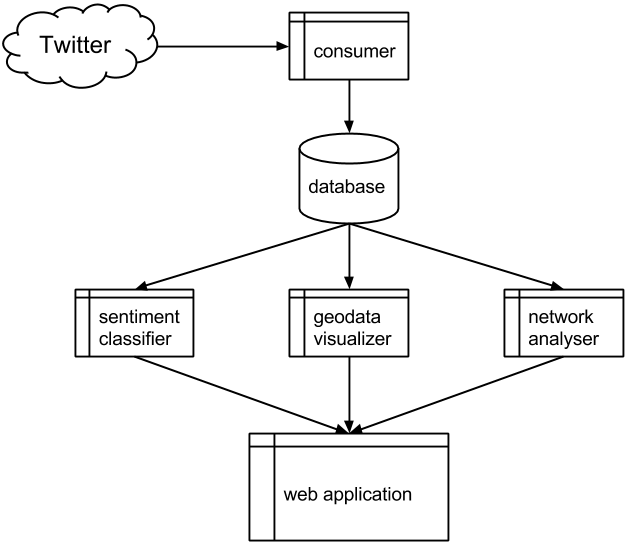
\includegraphics[width=140mm]{img/budowa-systemu.png}
\caption{Gruboziarnisty model systemu}
\label{image:gruboziarnisty-model-systemu}
\end{figure}

Każda z wyróżnionych powyżej części systemu bierze udział w innym etapie
badań. Na początku najważniejsze jest gromadzenie danych, po którym następuje
ich przetwarzanie by na końcu zająć się analizą i próba ekstrakcji wiedzy.
Wszystkie te części są ze sobą połączone wspólną bazą danych, w której
przechowywana jest zgromadzona wiedza i wyniki przetwarzania i analizy danych.
Poniżej pokrótce omówione są wszystkie z tych części.  

%%%%%%%%%%%%%%%%%%%%%%%%%%%%%%%%%%%%%%%%%%%%%%%%%%%%%%%%%%%% GROMADZENIE DANYCH
\section{Gromadzenie danych}
\label{section:gromadzeniedanych}
W tej sekcji opisuję sposób przeprowadzenia początkowych prac związanych
z moimi badaniami, które związane były ze zgromadzeniem danych potrzebnych
do przeprowadzania analiz. Etap ten był niezwykle istotny i przeprowadzenie
go umożliwiło dalsze prace. Zgromadzone dane pochodzą z serwisu Twitter
i zostały uzyskane przy pomocy udostępnionego publicznie API (interfejsu
programistycznego).

\subsection{Tematyka danych}
% piłka nożna, kibice
Aby przeprowadzić analizę danych koniecznym było wybranie podzbioru
użytkowników Twittera. Dwa aspekty zadecydowały o tym, że skupiono się nad
analizą anglojęzycznego środowiska piłkarskiego:
\begin{itemize}   
  \item struktura językowa użytkowników sieci Twitter -- według badań firmy Gnip
  \cite{GnipTwitterLanguages} (zajmującej się gromadzeniem danych z tego serwisu
  społecznościowego) w 2013 roku ponad 50\% tweetów wysłanych zostało w języku
  angielskim.
  Dla porównania w języku polskim było to zaledwie 0.11\%.
  Dlatego też badanie użytkowników anglojęzycznych ma największy sens, gdyż
  prowadzi do zebrania największej liczby tweetów.
  Wybór konkretnego języka komunikacji jest o tyle istotny, iż wpływa znacznie
  na część badań związaną z analizą sentymentu,
  \item dynamika wpisów na Twitterze -- w związku z narzuconym w serwisie
  ograniczeniem na liczbę znaków wpisu (140) oraz sposobem ich prezentowania
  użytkownikom na ich stronie głównej (chronologicznie od najnowszych) serwis
  ten charakteryzuje się wysoką dynamiką informacji wysyłanych przez użytkowników.
  Wpisy bardzo często odnoszą się do aktualnych wydarzeń, krótko je komentując.
  W związku z tym badanie środowiska piłkarskiego ma duży sens, gdyż zainteresowani
  futbolem internauci mają wiele tematów do dyskusji -- komentowanie spotkań na żywo,
  refleksje po meczach i dyskusje między spotkaniami.
  W profesjonalnych ligach piłkarskich mecze odbywają się co najmniej raz w tygodniu,
  a informacje o stanie kadrowym, kontuzjach i nadziejach przed meczem
  rozpalają kibiców swoich drużyn. W związku z wysoką dynamiką świata piłkarskiego,
  użytkownicy Twittera będący kibicami tworzą proporcjonalnie dużą liczbę
  tweetów -- komentując na biężąco wszelkie wydarzenia. Dlatego też wybór
  tej podgrupy do moich badań jest racjonalny i daje możliwość zbadania 
  zachowań użytkowników społecznościowych dostarczając wiele wpisów, na których
  można przeprowadzić analizy.
\end{itemize}  


\subsection{Sposób zbierania danych}
% wybrane kluby, słowa kluczowe, API, nasłuchiwanie
Aby uzyskać jak najlepsze rezultaty zbierania danych ze środowiska piłkarskiego
(posługującego się językiem angielskim) jako dziedzinę badań wybrano
najwyższą klasę rozgrywek piłki nożnej mężczyzn w Anglii (i Walii),
czyli Premier Leauge -- uznawaną przez wielu ekspertów za najsilniejszą ligę na
świecie. Co istotne, jest to także najczęściej oglądana liga piłkarska.
Średnio pojedynczy mecz ma widownię ponad 12 milionów osób
(\cite{PremierLeagueAudience}) bijąc ponad dwukrotnie oglądalność innych lig 
(włoskiej, hiszpańskiej czy niemieckiej).

Zbieranie danych odbywało się przy pomocy Twitter Stream API -- oficjalnie
udostępnionego interfejsu programistycznego.
Aby móc zbierać wpisy należy napisać program -- robota internetowego,
korzystającego z API, który nasłuchuje na żywo pojawiających się wpisów.

Technika ta ma jednak ograniczenia i pozwala na konsumowanie maksymalnie 1\%
wszystkich pojawiających się w tym czasie wpisów na Twitterze (aby uzyskać
wszystkie wpisy należy wnieść opłatę w serwisach partnerskich).

Do nasłuchiwania wpisów koniecznym jest także zdefiniowanie filtrów
określających jakie dane nas interesują. Twitter wymaga by podać przynajmniej
jeden z niniejszych: słowa kluczowe, identyfikatory użytkowników lub obszary
geograficzne. Dodatkowo możliwe jest podanie innych parametrów, jak na przykład
języka wpisów. Dlatego też zdecydowałem się korzystać z filtra słów kluczowych
wraz z ograniczeniem wpisów na język angielski.

Twitter Stream API dostarcza jedynie tweetów pojawiających się w czasie
rzeczywistym. Oznacza to, że możemy przy jego użyciu mieć jedynie dostęp do tych
wpisów, które zostały wysłane, gdy jednocześnie uruchomiony był nasz program
nasłuchujący. Aby zmaksymalizować jakość i zakres zebranych danych program
nasłuchujący uruchamiany był w trakcie odbywania się meczów 
(z kilkudziesięciuminutowym zapasem czasowym przed i po spotkaniu).

W związku z koniecznością określania słów kluczowych ograniczono liczbę
śledzonych klubów do najlepszej czwórki sezonu 2012/2013, którą tworzą:
Manchester United FC, Manchester City FC, Chelsea FC oraz Arsenal FC.
Są to więc odpowiednio dwa kluby z Manchesteru i dwa z Londynu.

Mecze nasłuchiwano od 23 listopada do 29 grudnia 2013 roku. W tym czasie odbyło
się 9 kolejek spotkań (od 12 do 19 kolejki włącznie). Jako słowa kluczowe przed
każdym meczem definiowane były: nazwiska i znane określenia
piłkarzy, nazwiska i znane określenia trenerów (menadżerów) drużyn, nazwy i
określenia klubów, nazwisko głównego sędziego i nazwa stadionu. 
Oprócz meczów Premier League nasłuchiwano także dwóch kolejek Ligi Mistrzów
z udziałem wyżej wymienionych zespołów, które odbyły się w tym czasie.

\clearpage
%%%%%%%%%%%%%%%%%%%%%%%%%%%%%%%%%%%%%%%%%%%%%%%%%%%%%%%%%%%% ANALIZA SENTYMENTU
\section{Analiza sentymentu}
\label{section:analizasentymentu}
W tym miejscu opisuję sposób w jaki została użyta do moich badań analiza
wydźwięku wypowiedzi. Przedstawiam czynności wstępne jakie zostały zastosowane
na tekście, prezentuję krótko wybrany algorytm i zastosowane w nim modyfikacje
oraz opisuję sposób zaaplikowania analizy wydźwięku na zgromadzonych tweetach.

\subsection{Normalizacja tekstu}
% pozbycie się słów kluczowych, zaprzeczenia, retweety

W związku z tym, że wpisy są tworzone przez zwykłych użytkowników posiadają one
wiele znaków i elementów, które z punktu widzenia analizy sentymentu są zbędne,
a czasami prowadzące do błędów. Dlatego też tekst należy poddać normalizacji,
usunięciu zbędnych elementów, szumów i spamu. Przykładowa lista wpisów jakie
znalazły się w zgromadzonych danych przedstawia poniższa tabela
(\ref{tab:wpisy-przed-normalizacja}).


\begin{table}[ht!]  
\begin{center}  
\begin{tabular}{|r|p{140mm}|}
\hline
\multicolumn{2}{|c|}{Przed normalizacją}
\\ \hline
1 & RT @J\_SPEKZ: Haha quality! \#Fellaini \#United \#Moyes
http://t.co/rJB4K1fvZy
\\ \hline
2 & Stay woke brah! The Arsenal is about to make everything alright soon :) RT
@JCphoenixx: So damn tired, So not sleepy.
\\ \hline
3 & @abdul1haseeb My arsenal is not disappointing too :P 
\\ \hline
4 & @Arsenal didn't think i could respect @aaronramsey any more than i already
did, bute what a gentleman he is for not to celebrate that goal:) 
\\ \hline
5 & BENDTNER!!! ARE YOU FUCKING SERIOUS!! Even though im not arsenal fan :o
\\ \hline
6 & Haha, you gotta agree, no one gets booed like Manchester United :D \#ZeDevilza
\\
\hline
\end{tabular} 
\end{center} 
\caption{Przykładowa lista wpisów przed normalizacją}
\label{tab:wpisy-przed-normalizacja}
\end{table}


Po przeprowadzeniu wszystkich prac związanych z normalizacją tekstu wpisy z
powyższej tabeli prezentują się w następujący sposób:

\begin{table}[ht!]  
\begin{center}  
\begin{tabular}{|r|p{140mm}|}
\hline
\multicolumn{2}{|c|}{Po normalizacji}
\\ \hline
1 & 
\\ \hline
2 & Stay woke brah make alright
\\ \hline
3 & not\_disappointing
\\ \hline
4 & didnt not\_respect bute gentleman not\_celebrate not\_goal
\\ \hline
5 & FUCKING im not\_fan
\\ \hline
6 & haha gotta agree not\_booed
\\
\hline
\end{tabular} 
\end{center} 
\caption{Lista wpisów poddanych normalizacji}
\label{tab:wpisy-po-normalizacja}
\end{table}

\clearpage
Kolejne kroki, które przekształciły tweety do powyższej postaci to:
\begin{enumerate}
  \item Usunięcie skomentowanych retweetów.\\
  \texttt{Stay woke brah! The Arsenal is about to make everything
  alright soon :) \sout{RT @JCphoenixx: So damn tired, So not sleepy.}}
  
  \item Usunięcie skomentowanych cytowań. \\
  \texttt{At all...\sout{"@dotun\_somoye: Even city's first goal
  negredo was offside....:( the refs not helping at all"} }
  
  \item Usunięcie hiperlinków.\\
  \texttt{You up for Arsenal's match later on? - what time? maybe if i'm not
  busy baby sitting :) \sout{http://t.co/aC5Ec8ipy1}}
 
  
  \item Usunięcie nazw użytkowników.\\
  \texttt{\sout{@abdul1haseeb} My arsenal is not disappointing too :P}
  
  
  \item Usunięcie hashtagów. \\
  \texttt{Haha, you gotta agree, no one gets booed like Manchester United :D
  \sout{\#ZeDevilza}}
  
  
  \item Oznaczenie wyrazów zaprzeczonych przedrostkiem \texttt{NOT\_} (opisuję
  dokładniej w sekcji \ref{subsection:sentyment-algorytm}). \\
  \texttt{didn't \textbf{NOT\_think NOT\_i NOT\_could NOT\_respect NOT\_any 
  NOT\_more NOT\_than NOT\_i NOT\_already NOT\_did}, bute what a gentleman he 
  is for not \textbf{NOT\_to NOT\_celebrate NOT\_that NOT\_goal:)}}

 \item Zachowanie tylko znaków alfabetu:
  	\begin{itemize}
  		\item usunięcie zaimków dzierżawczych (\texttt{Helen's} $\to$ \texttt{Helen}),
  		\item usunięcie apostrofu ze skróconych zaprzeczeń (\texttt{don't} $\to$ \texttt{dont}),
  		\item normalizacja liter diakrytyzowanych (\texttt{José Mourinho} $\to$ \texttt{Jose
  		Mourinho})
  		\item usunięcie liczb i wszelkich znaków niealfabetycznych.
	\end{itemize}

  \texttt{You up for Arsenal\sout{'s} match later on\sout{? -} what
  time\sout{?} maybe if i\sout{'}m not busy baby sitting \sout{:)}} 
	
	\item Usunięcie wyrazów zdefiniowanych w stop liście (powszechne wyrazy danego
	języka, które mogą być pominięte nie tracąc jednocześnie żadnej informacji).
	Zastosowałem stop listę z serwisu \mbox{WebPageAnalyse.com} 
	(\cite{WebPageAnalyse}) zawierającą 528 słów.

	\texttt{\sout{You up for} Arsenal match \sout{later on what} time \sout{maybe if} 
 	im \sout{not} busy baby sitting}
	
	\item Usunięcie słów kluczowych, które użyte były do gromadzenia wpisów z
	Twittera -- czyli nazwisk piłkarzy, menadżerów, nazw klubów, itd.
	
	\texttt{\sout{BENDTNER} FUCKING im \sout{NOT\_arsenal} NOT\_fan}
	
\end{enumerate}





\subsection{Zastosowanie algorytmu}
\label{subsection:sentyment-algorytm}
% + dobór parametrów, emotikony, zaprzeczenia

Do przeprowadzenia analizy sentymentu na zebranych tweetach skorzystałem z
metody opracowanej przez Alexandra Paka i Patricka Paroubek'a, którą
krótko przedstawiłem w sekcji \ref{subsubsection:pakandparoubek}.
Jest to technika, która pozwala badać sentyment bez słownika sentymentu.
Pierwszym krokiem jest zbudowanie słownika z zebranych danych.
W tym celu wybiera się podzbiór wpisów, które zawierają emotikony.
W związku ze 140 znakowym ograniczeniem na długość znaków przyjmuje się
założenie, że dana emotikona nadaje wydźwięk całemu wpisowi.
Według artykułu \cite{EmoticonAnalysisTwitter} 20 emotikon pokrywa
w 90\% stosowanie tych znaków graficznych we wpisach (na 100 wpisów z
emotikonami, 90 z nich zawiera emotikonę ze zbioru tych 20). Dlatego też
skorzystałem z tego zbioru do własnych badań dzieląc emotikony na wyrażające
wydźwięk pozytywny i negatywny w następujący sposób \footnote{emotikona
\texttt{D:} została pominięta, gdyż pokrywała więcej przypadków niż tylko
użycie emotikony (np.: \texttt{Accepte\textbf{d:} Mary, John, Jane})}:

\begin{table}[ht!]  
\begin{center}  
\begin{tabular}{|c|r|l|}
\hline
Emotikona & Popularność & Wydźwięk
\\ \hline
\texttt{:)} & $33.4\%$ & pozytywny \\ \hline
\texttt{:D} & $11.0\%$ & pozytywny \\ \hline
\texttt{:(} & $7.9\%$ & negatywny \\ \hline
\texttt{;)} & $7.5\%$ & pozytywny \\ \hline
\texttt{:-)} & $4.4\%$ & pozytywny \\ \hline
\texttt{:P} & $3.7\%$ & pozytywny \\ \hline
\texttt{=)} & $3.7\%$ & pozytywny \\ \hline
\texttt{(:} & $2.8\%$ & pozytywny \\ \hline
\texttt{;-)} & $2.2\%$ & pozytywny \\ \hline
\texttt{:/} & $1.9\%$ & negatywny \\ \hline
\texttt{XD} & $1.9\%$ & pozytywny \\ \hline
\texttt{=D} & $1.5\%$ & pozytywny \\ \hline
\texttt{:O} & $1.1\%$ & pozytywny \\ \hline
\texttt{=]} & $1.1\%$ & pozytywny \\ \hline
\texttt{;D} & $1.0\%$ & pozytywny \\ \hline
\texttt{:]} & $1.0\%$ & pozytywny \\ \hline
\texttt{:-(} & $0.8\%$ & negatywny \\ \hline
\texttt{=/} & $0.8\%$ & negatywny \\ \hline
\texttt{=(} & $0.8\%$ & negatywny \\ \hline
\end{tabular} 
\end{center} 
\caption{Wydźwięk emotikon}
\label{tab:wydzwiek-emotikon}
\end{table}

Następnie przeglądnięto wszystkie tweety z emotikonami zliczając liczbę
występowania wyrazów w kontekście pozytywnym i negatywnym.
Najpierw badano sentyment całego wpisu (na podstawie emotikony -- gdy była ich
większa ilość wybierano ten sentyment, który przeważał) a następnie dla każdego
wyrazu z tego wpisu zwiększano licznik odpowiednio wystąpień pozytywnych lub
negatywnych. Oczywiście wpisy były już poddane normalizacji.
W ten sposób uzyskano słownik sentymentu zbudowany z zebranych danych, który
zawierał 34183 słowa, a najpopularniejsze z nich to:


\begin{table}[ht!]  
\begin{center}  
\begin{tabular}{|l|r|r|r|r|}
\hline
Słowo & Wyst. pozytywne  & Wyst. negatywne 
& Pozytywność\tablefootnote{Wartość liczona jako: \texttt{pozytywne / (pozytywne +
negatywne)} -- tylko na potrzeby niniejszej tabeli, nieużywana w algorytmie}
& Valence
\\ \hline 
win & 4206 & 598 & 87.6 \% & 0.845 \\ \hline
good & 3916 & 435 & 90.0 \% & 0.903 \\ \hline
game & 3016 & 1012 & 74.9 \% & 0.301 \\ \hline
goal & 2305 & 584 & 79.8 \% & 0.477 \\ \hline
today & 2019 & 526 & 79.3 \% & 0.477 \\ \hline
time & 1844 & 404 & 82.0 \% & 0.602 \\ \hline
dont & 1461 & 775 & 65.3 \% & 0.000 \\ \hline
match & 1669 & 449 & 78.8 \% & 0.477 \\ \hline
great & 1885 & 160 & 92.2 \% & 1.041 \\ \hline
love & 1837 & 202 & 90.1 \% & 0.954 \\ \hline
\end{tabular} 
\end{center} 
\caption{Liczba występowania najpopularniejszych słów w zbudowanych słowniku
sentymentu}
\label{tab:liczebnosc-slow-sentymentu}
\end{table}

Zgodnie z algorytmem wartość \textit{valence} używana jest w dalszych
obliczeniach. Dla każdego wpisu wyliczana jest średnia arytmetyczna tych
wielkości przypisanych do każdego słowa. Wynik ten jest wartością
\textit{valence} danego wpisu. Poniżej prezentuję przykładowe wyniki wyliczania
tej wielkości:
\clearpage
\begin{table}[ht!]  
\begin{center}  
\begin{tabular}{|p{12mm}|p{70mm}|>{\raggedright\arraybackslash}p{60mm}|}
\hline
Valence & Wpis & Składowe 
\\ \hline 
0.6261 POS & Just seen you in the crowd at Chelsea game! @domashman http://t.co/NjovoZdgZ3 & {game=0.4740, crowd=0.7782}
\\ \hline
0.5909 POS & RT @BTSP: \#PRIZEDRAW If Arsenal win tonight one lucky person
will win a personalised BTSP mug! Simply RT \& follow to enter!
http://t.co/9m... & {lucky=0.4613, tonight=0.6873, btsp=0.3010, person=0.4232, personalised=0.3010, enter=0.5351, follow=1.2229, win=0.8465, mug=0.4771, simply=0.3979}
\\ \hline
0.6199 POS & Liking the brightness of this Napoli kit \#tempted &
{liking=0.8062, kit=0.4337} \\ \hline
0.0305 NEG & @ricktaylor1987 You're not watching Arsenal? &
{not\_watching=0.0305} \\ \hline
0.1234 NEG & Poor start\#AFC & {poor=-0.2848, start=0.5317}
\\ \hline
0.1807 NEG & Do Arsenal have any players who don't fall down with ease?
\#SwimmingTeam & {players=0.3684, not\_fall=-0.3979, not\_ease=0.4771,
dont=0.2751} \\ \hline
\end{tabular} 
\end{center} 
\caption{Wynik działania algorytmu analizy sentymentu na przykładowych wpisach}
\end{table}

Określenie sentymentu wpisu odbywa się zgodnie z równaniem:
\begin{equation}
S(t) =
\begin{cases}
POS & valence(t) > AVG\_VALENCE \\
NEG & valence(t) <= AVG\_VALENCE \\
\end{cases}
\end{equation}
Wielkość $AVG\_VALENCE$ jest średnią arytmetyczną wartości $valence$
wszystkich wpisów. W moich badaniach wartość ta wyniosła $0.4786984978198536$.

\subsubsection{Wykrywanie i obsługa negacji}
W oryginalnym podejściu panów Pak i Paroubek nie ma żadnego sposobu na
wykrywanie i obsługę negacji. Oczywistym jednak jest, iż zaprzeczenia zmieniają
znaczenie dalszej części tekstu i muszą być w jakiś sposób obsłużone.
Wpisy na Twitterze są krótkie, więc postanowiłem zastosować podejście
zaprezentowane w artykule \cite{thumbsUp2002}, które polega na dodaniu
przedrostka \texttt{NOT\_} do wszystkich słów pomiędzy wyrazem negującym,
a najbliższym znakiem przestankowym. Lista wyrazów negujących
została zaczerpnięta z \cite{englishNots1983}. Słowa zanegowany miały osobno
liczone liczby wystąpień w kontekstach pozytwnych i negatywnych. W takiej formie
brały udział w ocenie sentymentu wpisów z Twittera.


\subsubsection{Dobór parametrów}
Użyty przeze mnie algorytm zakłada dobór parametrów przed przeprowadzeniem
analizy sentymentu. Parametry te dotyczą słów ze zbudowanego słownika --
decydując, które z nich wezmą udział w procesie analizy. Są to: minimalna
długość słowa, minimalna liczba występowania słowa. Doboru parametrów dokonałem
w sposób zaprezentowany w opisie algorytmu. Wykorzystałem listę wpisów z
emotikonami, podzieliłem je na zbiór uczący i testowy w stosunku 20\% do 80\%.
Wygenerowałem słownik ze zbioru uczącego. Wpisy ze zbioru testowego oznaczyłem spodziewanym
sentymentem -- był to sentyment emotikony jaką zawierały. Następnie
przeprowadziłem testy poprawności klasyifkacji zbioru testowego słowami ze
zbioru uczącego dla wyrazów o minimalnej długości od 1 do 10 i minimalnej
liczbie wystąpień od 1 do 100 -- daje to w sumie 1000 testów.
Najwyższy stopień poprawności klasyfikacji uzyskałem dla parametrów równych:
minimalna długość wyrazu -- 3, \mbox{minimalna częstotliwość wystąpień -- 1}.
Wyniki testów przedstawiam na poniższym wykresie
\ref{image:pak-paroubek-parametry}.

\begin{figure}[ht!]
\centering
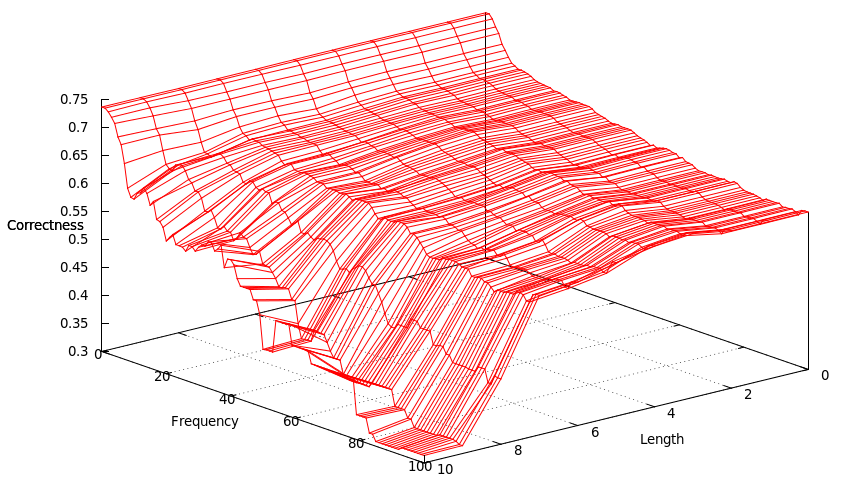
\includegraphics[width=140mm]{img/pak-paroubek-params.png}
\caption{Dobór parametrów algorytmu analizy sentymentu}
\label{image:pak-paroubek-parametry}
\end{figure}

% %%%%%%%%%%%%%%%%%%%%%%%%%%%%%%%%%%%%%%%%%%%%%%%%%%% ANALIZA SIECI SPOŁECZNYCH
\section{Analiza sieci społecznych}
\label{section:siecispoleczne}
W tej sekcji przedstawiam zastosowane podejście do analizy sieci społecznych,
odkrywania sieci społecznych z zebranych danych oraz sposoby na wykrywanie grup
i badanie podobieństw między sieciami.
\subsection{Budowa sieci społecznych z danych z Twittera}
% wykorzystanie reply, retweet
Relacje między użytkownikami na Twitterze zbudowane są na modelu jednostronnym.
Oznacza to, że każdy posiada dwie listy -- osób, które obserwuje oraz osób,
przez które jest obserwowany (\textit{following} i \textit{followers}).
Są to listy statyczne, budowanie ręcznie przez użytkowników tego portalu
mikroblogowego. Twitter ukierunkowany jest jednak na swobodną komunikację między
wszystykimi użytkownikami -- dlatego kontakty między nimi nie są ograniczone
tylko do osób, które mamy na którejść z list. Nie ma żadnego problemu by jeden
użytkownik komunikował się z drugim, gdy oboje nie mają się na żadnej z list.
Najczęściej komunikacja ta odbywa się publicznie poprzez pisanie tweetów między
sobą, odpowiadanie na wpisy innych użytkowników. Aby uzyskać lepsze efekty
pokazując tworzące się grupy społeczne ukierunkowałem swoje prace na relacje
tworzone w trakcie interakcji między użytkownikami poprzez odpowiedzi i
retweety.

Korzystając ze Streaming API pobierającego tweety otrzymywałem również
informację o tym, do kogo skierowana jest odpowiedź w przypadku takiego rodzaju
wpisu.
W polu \texttt{in\_reply\_to\_user\_id} znajdował się unikalny numer ID
użytkownika, do którego odpowiedź była skierowana, zaś w polu \texttt{user\_id}
ID autora odpowiedzi. 
Oprócz odpowiedzi istotne również były wpisy typu retweet. Przykładowy wpis tego
typu wygląda następująco: \texttt{RT @AHeryantooo: Keep calm and trust in Moyes. Gapapa Yes ;;)}.
Aby z takiego wpisu pobrać ID użytkownika, którego wpisu został retweetowany -- w tym
przypadku jest to użytkownik \texttt{@AHeryantooo}, przeglądałem tabelę z użytkownikami
i przypisywałem do tego rodzaju wpisów wartość pola \texttt{retweeted\_user\_id}
jako znalezione ID konkretnego użytkownika.

Korzystając z tych dwóch rodzajów połączeń między użytkownikami byłem w stanie 
odkryć relacje między nimi. Naturalnym rodzajem traktowania tych danych było
uznanie użytkowników (de facto ich numerów ID) za wierzchołki, a relacje między nimi
(\texttt{in\_reply\_to\_user\_id} oraz \texttt{retweeted\_user\_id}) za krawędzie
w grafie.

 \subsection{Wykrywanie grup i badanie podobieństwa}
 \label{section:koncepcja-wykrywaniegrup}
% gephi, modularity
Do wykrywania grup wśród sieci społecznych skorzystałem z narzędzia
otwartoźródłowego narzędzia \textit{Gephi} wspomagającego analizę grafową, w
którym został zaimplementowany algorytm przedstawiony w artykule
\cite{blondel2008fuc}. Przy jego użyciu konkretne węzły zostały podzielone
na grupy, nad którymi przeprowadzałem późniejsze analizy.



Badanie podobieństwa oparte było o analizę kolejnych wydarzeń. 
Polegało polegało na zliczeniu ile wierzchołków powtarza się w kolejnych meczach.
Oparte zostało o niniejsze równanie:
\begin{equation}
S = \frac{|V_1 \cap V_2|}{|V_1|}
\end{equation}  
gdzie $V_1$ to zbiór wierzchołków w pierwszym wydarzeniu, a $V_2$ w drugim.
Krótko mówiąc podobieństwo to iloraz liczby wspólnych wierzchołków między 
wydarzeniami a liczby wierzchołków w pierwszym z nich.


\begin{comment}
Badanie podobieństwa oparte było głównie o analizę kolejnych wydarzeń.
W tym celu zastosowałem dwa podejścia. Pierwsze oparte na wszystkich
wierzchołkach (użytkownikach) polegało na zliczeniu ile z nich się powtarza.
Podobieństwo między kolejnymi meczami zostało oparte o niniejsze równanie:
\begin{equation}
S = \frac{|V_1 \cap V_2|}{|V_1 \cup V_2|}
\end{equation}  
gdzie $V_i$ to zbiór wierzchołków w wydarzeniu $i$. Krótko mówiąc podobieństwo
to iloraz liczby wspólnych wierzchołków między wydarzeniami a liczby sumy 
wierzchołków tych wydarzeń.
Drugie podejście zostało zastosowane do znalezionych przy pomocy \textit{Gephi} 
grup. Bada ono podobieństwo pomiędzy grafami, uwzględniając zarówno wierzchołki
jak i krawędzie. Jest to opracowany przez mnie algorytm, który można wyrazić
wzorem:
\begin{equation}
S = \frac{E_1 \cap E_2}{E_{V_1 \cap V_2}} \cdot \frac{V_1 \cap V_2}{V_1 \cup V_2}
\end{equation}
gdzie $E_i$ oznacza krawędzie w grafie $i$, $V_i$ wierzchołki w grafie $i$,
natomiast $E_{V_1 \cap V_2}$ oznacza wszystkie krawędzie między wspólnymi 
wierzchołkami. Poniżej przedstawiam przykład zastosowania powyższego algorytmu.

\clearpage
Wyniki podobieństwa między grafami zaprezentowane są na rysunku 
\ref{image:podobienstwo-grafow}.

\begin{figure}[ht!]
\centering
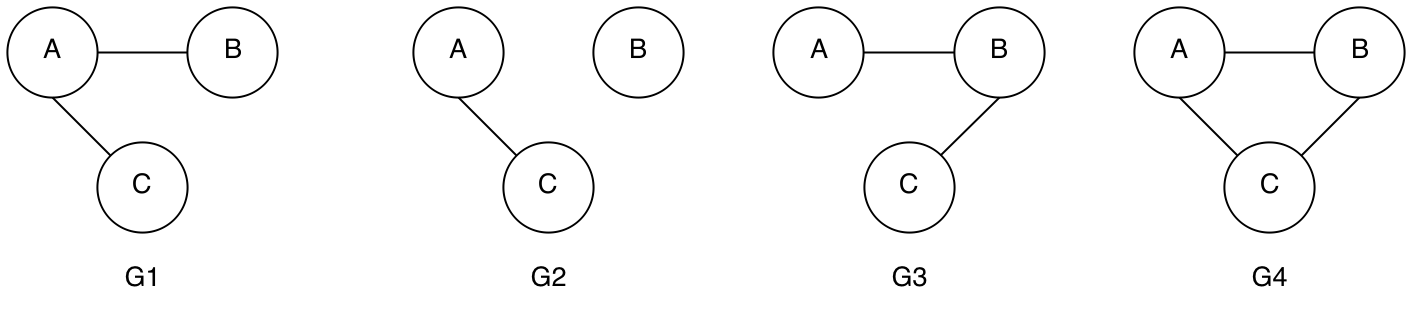
\includegraphics[width=140mm]{img/podobienstwo-grafow.png}
\caption{Przykładowe grafy do przedstawienia algorytmu podobieństwa}
\label{image:podobienstwo-grafow}
\end{figure}

\begin{table}[ht!]  
\begin{center}  
\begin{tabular}{|l|l|p{40mm}|p{40mm}||p{21mm}|}
\hline
Graf 1 & Graf 2 & Wsp. krawędzie / Krawędzie między wsp. wierzchołkami ($X_1$) & 
	Wsp. wierzchołki / Suma wierzchołków ($X_2$) & Podobieństwo ($X_1 \cdot X_2$)
\\ \hline 
G1 & G2 & 1 / 2 & 3 / 3 & 50.0 \% 
\\ \hline 
G1 & G3 & 1 / 3 & 3 / 3 & 33.3 \% 
\\ \hline 
G2 & G3 & 0 / 3 & 3 / 3 &  0.0 \%
\\ \hline 
G1 & G4 & 2 / 3 & 3 / 3 & 66.7 \%
\\ \hline
\end{tabular} 
\end{center} 
\caption{Przykładowe wyniki algorytmu podobieństwa grafów}
\end{table}

\end{comment}

%%%%%%%%%%%%%%%%%%%%%%%%%%%%%%%%%%%%%%%%%%%%%%%%%%%%%% WYKORZYSTANIE GEOLOKACJI
\section{Wykorzystanie geolokacji}
\label{section:wykorzystaniegeolokacji}
% tweety z geolokacją
% wyciąganie informacji o miejscu - Open Street Map
% zastosowanie: odl. między użytkownikiami, od stadionu, dzielnice
W danych pobieranych z Twittera w części wpisów znajdowały się informacje o 
geolokacji -- współrzędne długości i szerokości geograficznej, z której
dany wpis został wysłany. Wykorzystanie tych informacji zostało zastosowane
do wzbogacenia analiz przeprowadzonych na zebranych danych. Informacje
o położeniu użytkowników bardzo często zbiegały się z miejscem rozgrywania meczu.
W bazie danych miałem jednak tylko informacje o danych geograficznych.
Aby wzbogacić je o więcej wiedzy postanowiłem skorzystać z projektu
Open Street Map (\textit{http://www.openstreetmap.org}).
Przy pomocy API, które projekt ten udostępnia udało mi się ubogacić dane
na temat lokalizacji o informacje opisowe miejsca, o które chodzi.
Poprzez \textit{Reverse Geocoding} możliwe było podając współrzędne
goegraficzne uzyskać między innymi takie informacji o adresie jak:
kraj (ang. \textit{country}), stan/państwo (ang. \textit{state}), 
hrabstwo (ang. \textit{county}), miasto (ang. \textit{city}).

Dodatkowo wykorzystanie geolokacji może być użyte do zbadania odległości między 
użytkownikami tworzącymi sieć społeczną, o tym w jakiej odległości są oni od stadionu,
czy również do zbadania sentymentu w zależności od wydarzeń na boisku,
a miejscem przebywania danych użytkowników. 













\chapter{Architektura, technologie, narzędzia}
\label{chapter:architektura}
W tym rozdziale opisuję krótko architekturę zbudowanego systemu.
W sekcji \ref{section:architekturasystemu} opisuję ogólną architekturę,
w \ref{section:zastosowanetechnologie} omawiam technologie, które zastosowałem,
a w ostatniej części \ref{section:bibliotekiinarzedzia} wymieniam użyte
biblioteki i narzędzia.
\section{Architektura systemu}
\label{section:architekturasystemu}

\begin{figure}[ht!]
\centering
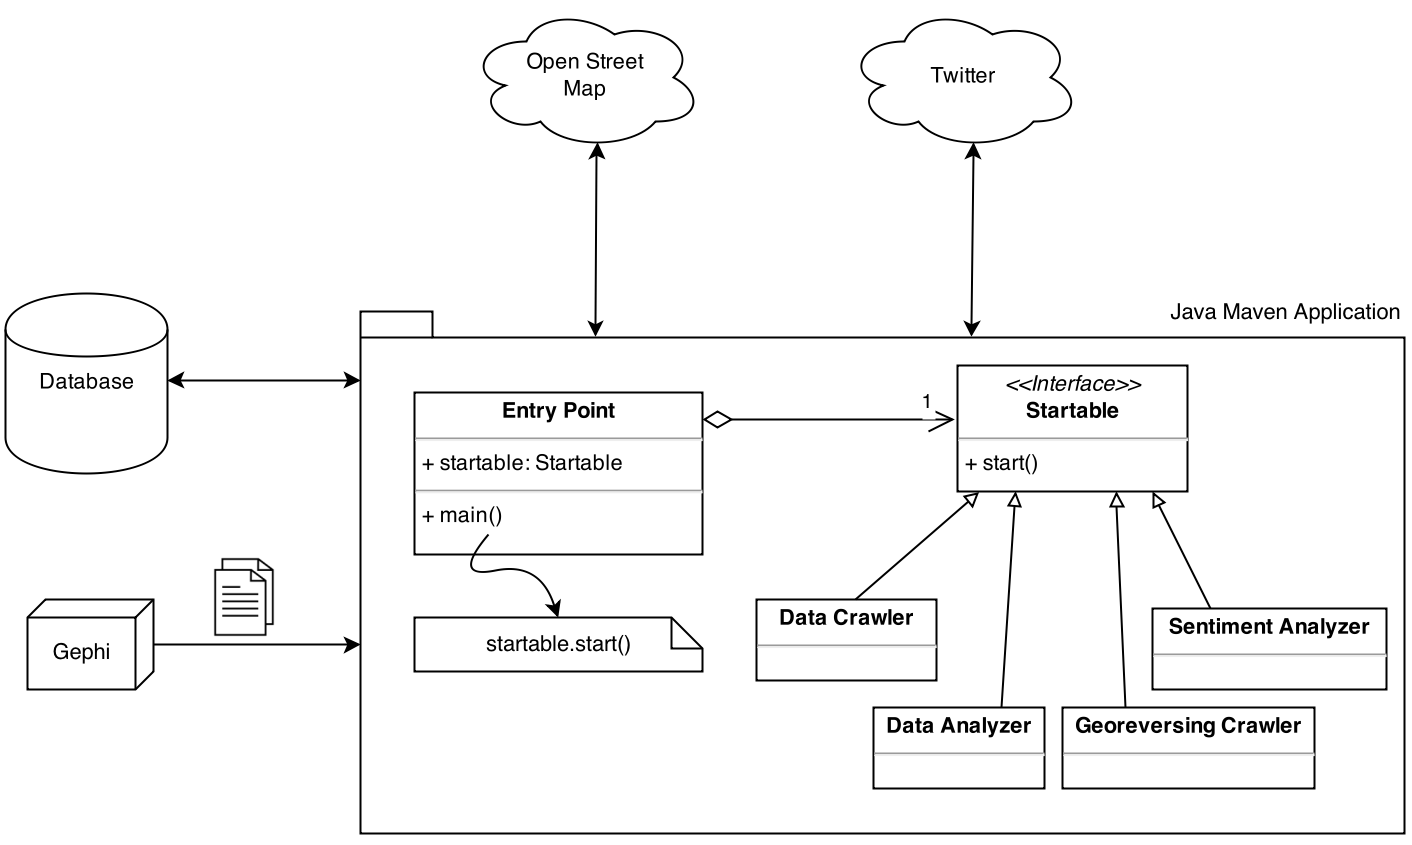
\includegraphics[width=160mm]{img/architektura.png}
\caption{Architektura systemu}
\label{image:architektura-systemu}
\end{figure}
Systemu została zbudowany na pojedynczej aplikacji Javowej,
w której zostały zaimplementowane wszystkie potrzebne operacje.
Aplikacja ta komunikuje się z pojedynczą bazą danych, w której zawarte
są wszystkie wpisy potrzebne zarówno do zbierania danych jak i te, które są
wynikiem analiz. Dodatkowo odpowiada ona za komunikację z usługami w chmurze --
czyli zbieraniem danych z Twittera i \textit{georeversingiem} lokacji z Open
Street Map. Wszystkie analizy zebranych danych również zostały przeprowadzone
przy użyciu aplikacji Javowej.

Oprócz aplikacji Javowej wykorzystano także program Gephi, które wyniki zapisano
do plików, a następnie przy użyciu wyżej wymienionej aplikacji przeparsowano i
umieszczono w bazie danych.

Wewnątrz aplikacji zaimplementowano między innymi moduł do zbierania danych z
Twittera (na podstawie podanych słów kluczowych), moduł związany z
przeprowadzeniem całego procesu analizy sentymentu -- od budowy słownika, do
zanalizowania pojedynczych wpisów, moduł związany z analizą zebranych danych,
a także kod odpowiedzialny za operacje związane z geolokacją.

\section{Zastosowane technologie}
\label{section:zastosowanetechnologie}
% java, postgres, sql, git
Jak już zostało wspomniane wyżej, główną technologią użytą podczas prac był
język Java. Oprócz niego wymienić należy także:
\begin{itemize}
  \item baza danych -- PostgreSQL,
  \item budowanie aplikacji -- Apache Maven,
  \item system kontroli wersji -- Git z repozytorium na GitHub (www.github.com).
\end{itemize}
\section{Wykorzystane biblioteki i narzędzia}
\label{section:bibliotekiinarzedzia}
% Twitter API, CartoDB, OSMap, GMap, GCharts, CartoDB, Gephi
Najważniejsze biblioteki, z których skorzystałem to:
\begin{itemize}
  \item Twitter4J -- biblioteka Javowa ułatwiająca korzystanie z Twitter API,
  użyta do zbierania \mbox{danych z Twittera,}
  \item Hibernate -- framework ORM\footnote{Object Relational Mapping --
  mapowanie obiektowo relacyjne} do komunikacji z bazą danych,
  \item Google Guice, JBoss Weld -- biblioteki pozwalające zastosować
  wstrzykiwanie zależności w aplikacji Javowej,
  \item Google Guava, Apache Commons, Apache Log4J, Joda Time -- biblioteki
  usprawniające programowanie w Javie,
  \item JUnit -- framework do pisania i uruchamiana testów automatycznych.
\end{itemize}
\chapter{Opis przeprowadzonych eksperymentów}
\label{chapter:eksperymenty}
% plan eksperymentow, opis danych, wyniki i wnioski
W niniejszym rozdziale przedstawione są eksperymenty, które zostały
przeprowadzone na zebranych wcześniej danych.
Opisany jest sposób ich wykonania, wyniki i wnioski.
Na początku w rozdziale \ref{section:opisdanych} opisana jest charakterystyka
zebranych danych, a następnie opisuję eksperymenty związane z analizą sentymentu
\ref{section:analizasentymentu2}, analizą społeczną 
\ref{section:analizaspoleczna} i analizą geolokacji 
\ref{section:analizageograficzna}.














%%%%%%%%%%%%%%%%%%%%%%%%%%%%%%%%%%%%%%%%%%%%%%%%%%%%%%%%%%%%%%%%%%% OPIS DANYCH
\section{Opis zebranych danych}
\label{section:opisdanych}
% 300 slow kluczowych, 18 druzyn, 50 meczow, daty,
% 7 mln tweetów, z tego 300 bylo retweetow, 800 z geolokacja, itd

Pomiędzy październikiem a grudniem 2013 roku zebrano 7 263 523 tweety związane
z piłką nożną. Pierwszy z nich ma datę 23 października 15:35:24 a ostatni
29 grudnia 19:27:27. Wszystkie wpisy są powiązane z rozegranymi w tym czasie
35 spotkaniami klubów Arsenal F.C. , Chelsea F.C., Manchester United F.C. i
Manchester City F.C. Daje to średnio 207 529 tweetów na mecz i niecałe
1 815 880 tweetów na drużynę.

Do zbierania tweetów użyte zostały dane 30 drużyn z 538 piłkarzami.
Dodając do tego popularne określenia menadżerów, piłkarzy czy klubów sumarycznie
zebrano 777 słów kluczowych, co daje średnio 22 słowa kluczowe na mecz.

Wpisy zostały stworzone przez 1 567 435 użytkowników, co daje 4.6 
wpisu na użytkownika. \mbox{222 545 wpisów} zawiera informacje o geolokacji, co 
stanowi zaledwie 3.06\% liczby wszystkich wpisów. \mbox{666 199 wpisów} to 
odpowiedzi (ang. \textit{replies}), to jest 9.17\%, natomiast aż 3 143 060 
tweetów jest retweetami pokrywając 43.27\% danych.

W tabeli \ref{table:listameczow} prezentuję listę wszystkich meczów, które były 
nasłuchiwane wraz z podstawowymi informacjami na ich temat.



\clearpage

\begin{table}[ht!]  
\begin{center}  
\begin{tabular}{|r|l|l|l|r|r|}
\hline
Lp. & Data & Gospodarz & Gość & Tweetów & Geolok.
\\ \hline 
1 & 2013-11-23 16:00 & Arsenal Londyn & Southampton FC & \texttt{190028} & \texttt{5231}	\\ \hline
2 & 2013-11-26 20:45 & FC Basel & Chelsea Londyn & \texttt{121209} & \texttt{3339}	\\ \hline
3 & 2013-11-26 20:45 & Arsenal Londyn & Olympique Marseille & \texttt{185252} & \texttt{6255}	\\ \hline
4 & 2013-11-27 20:45 & Manchester City & Viktoria Plzen & \texttt{24990} & \texttt{792}	\\ \hline
5 & 2013-11-27 20:45 & Bayer Leverkusen & Manchester United & \texttt{199232} & \texttt{6242}	\\ \hline
6 & 2013-11-30 16:00 & Cardiff City FC & Arsenal Londyn & \texttt{233151} & \texttt{6316}	\\ \hline
7 & 2013-12-01 13:00 & Tottenham Hotspur & Manchester United & \texttt{166394} & \texttt{4628}	\\ \hline
8 & 2013-12-01 17:10 & Chelsea Londyn & Southampton FC & \texttt{241768} & \texttt{7536}	\\ \hline
9 & 2013-12-01 17:10 & Manchester City & Swansea City & \texttt{29977} & \texttt{785}	\\ \hline
10 & 2013-12-04 20:45 & Sunderland AFC & Chelsea Londyn & \texttt{60047} & \texttt{1997}	\\ \hline
11 & 2013-12-04 20:45 & Manchester United & Everton FC & \texttt{182406} & \texttt{6226}	\\ \hline
12 & 2013-12-04 20:45 & Arsenal Londyn & Hull City & \texttt{200456} & \texttt{5076}	\\ \hline
13 & 2013-12-04 21:00 & West Bromwich Albion & Manchester City & \texttt{17783} & \texttt{608}	\\ \hline
14 & 2013-12-07 13:45 & Manchester United & Newcastle United & \texttt{416647} & \texttt{12613}	\\ \hline
15 & 2013-12-07 16:00 & Stoke City & Chelsea Londyn & \texttt{148780} & \texttt{4337}	\\ \hline
16 & 2013-12-07 16:00 & Southampton FC & Manchester City & \texttt{48101} & \texttt{1481}	\\ \hline
17 & 2013-12-08 17:00 & Arsenal Londyn & Everton FC & \texttt{381568} & \texttt{13057}	\\ \hline
18 & 2013-12-10 20:45 & Manchester United & Shakhtar Donetsk & \texttt{180301} & \texttt{6264}	\\ \hline
19 & 2013-12-10 20:45 & Bayern Monachium & Manchester City & \texttt{145381} & \texttt{4957}	\\ \hline
20 & 2013-12-11 20:45 & Chelsea Londyn & Steaua Bucuresti & \texttt{66125} & \texttt{1767}	\\ \hline
21 & 2013-12-11 20:45 & Napoli & Arsenal Londyn & \texttt{225461} & \texttt{7359}	\\ \hline
22 & 2013-12-14 13:45 & Manchester City & Arsenal Londyn & \texttt{525799} & \texttt{15561}	\\ \hline
23 & 2013-12-14 16:00 & Chelsea Londyn & Crystal Palace & \texttt{90541} & \texttt{2889}	\\ \hline
24 & 2013-12-15 14:30 & Aston Villa & Manchester United & \texttt{217221} & \texttt{6486}	\\ \hline
25 & 2013-12-21 16:00 & Manchester United & West Ham United & \texttt{171947} & \texttt{3975}	\\ \hline
26 & 2013-12-21 16:00 & Fulham FC & Manchester City & \texttt{63624} & \texttt{1624}	\\ \hline
27 & 2013-12-23 21:00 & Arsenal Londyn & Chelsea Londyn & \texttt{622011} & \texttt{19033}	\\ \hline
28 & 2013-12-26 13:45 & Hull City & Manchester United & \texttt{307313} & \texttt{8056}	\\ \hline
29 & 2013-12-26 16:00 & Chelsea Londyn & Swansea City & \texttt{109200} & \texttt{3264}	\\ \hline
30 & 2013-12-26 16:00 & West Ham United & Arsenal Londyn & \texttt{275811} & \texttt{8276}	\\ \hline
31 & 2013-12-26 18:30 & Manchester City & Liverpool FC & \texttt{331574} & \texttt{12009}	\\ \hline
32 & 2013-12-28 16:00 & Manchester City & Crystal Palace & \texttt{70251} & \texttt{2057}	\\ \hline
33 & 2013-12-28 16:00 & Norwich City & Manchester United & \texttt{204775} & \texttt{5348}	\\ \hline
34 & 2013-12-29 14:30 & Newcastle United & Arsenal Londyn & \texttt{339908} & \texttt{10624}	\\ \hline
35 & 2013-12-29 17:00 & Chelsea Londyn & Liverpool FC & \texttt{468494} & \texttt{16477}	\\ \hline
\end{tabular} 
\end{center} 
\caption{Lista meczów, które były nasłuchiwane}
\label{table:listameczow}
\end{table}





















%%%%%%%%%%%%%%%%%%%%%%%%%%%%%%%%%%%%%%%%%%%%%%%%%%%%%%%%%%%% PLAN EKSPERYMENTÓW
\section{Plan eksperymentów}
W ramach eksperymentów chciałem udowodnić sensowność zastosowania zarówno
analizy sentymentu jak i geolokacji w analizie użytkowników sieci 
społecznościowych. Przedstawię serię badań pokazujących w jaki sposób
można połączyć te trzy dziedziny by odkrywać wiedzę dotyczącą sieci
społecznych. Pokażę do czego można użyć sentymentu, do czego geolokacji
i w jaki sposób je połączyć.

Plan eksperymentów wygląda następująco:
\begin{itemize}
  \item wartość sentymentu w kolejnych meczach 
  \ref{subsection:sentymentwmeczach},
  
  \item aktywność użytkowników i sentyment w ciągu meczu
  \ref{subsection:aktywnoscwmeczu},
  
  \item sposoby komunikacji między zwolennikami i przeciwnikami klubu 
  \ref{subsection:rodzajekomunikacji},
  
  \item sentyment wypowiedzi w relacjach między użytkownikami
  \ref{subsection:sentymentwrelacjach},
  
  \item struktura grup użytkowników w kolejnych meczach
  \ref{subsection:strukturagrup},
  
  \item odległość między użytkownikami a częstość kontaktów
  \ref{subsection:odlegloscmiedzyuzytkownikami},
  
  \item rozkład wpisów na mapie świata
  \ref{subsection:rozkladnamapie},
  
  \item odległość kibiców od miejsca rozgrywania meczu
  \ref{subsection:odlegloscodstadionu},
  
  \item rozkład wpisów z geolokacją
  \ref{subsection:geowpisy}.
\end{itemize}

Eksperymenty zostały przeprowadzone dla wszystkich badanych drużyn.
Ich wyniki były do siebie zbliżone, dlatego przedstawiam je tylko dla części z
nich.



% %%%%%%%%%%%%%%%%%%%%%%%%%%%%%%%%%%%%%%%%%%%%%%%%%%%%%%%%%%% ANALIZA SENTYMENTU
\section{Analiza sentymentu}
\label{section:analizasentymentu2}
% 40\% bylo pozytywnych, 30\% negatywnych w meczach Arsenalu byl taki a taki sentyment

Analiza sentymentu została przeprowadzona zgodnie z algorytmem przedstawionym w
rozdziale \ref{subsubsection:pakandparoubek}. W związku z tym, że wpisy typu
retweet nie mogą posiadać sentymentu wszystkie zaprezentowane poniżej analizy
odnoszą się do grupy wpisów nie będących retweetami. To daje nam 4 120 463
tweety, nad którymi były prowadzone badania. W tej grupie 2 005 934 wpisy
zostały oznaczone jako pozytywne -- 48.68\%, a 1 944 448 jako negatywne --
47,19\%.



\subsection{Sentyment w meczach}
\label{subsection:sentymentwmeczach}
Pierwszym eksperymentem jaki został przeprowadzony było zbadanie tego w jaki 
sposób zmienia się wydźwięk wypowiedzi pomiędzy kolejnymi meczami danej drużyny.
W tym celu zbadany został ogólny sentyment podczas danego wydarzenia sportowego.
Na wykresach \ref{image:pozytywnosc-arsenal} oraz 
\ref{image:pozytywnosc-munited} przedstawione są wyniki tych badań.
Wartość pozytywności została wyliczone zgodnie z opisem w rozdziale
\ref{subsection:ocenapozytywnosci}.

\clearpage

\begin{figure}[ht!]
\centering
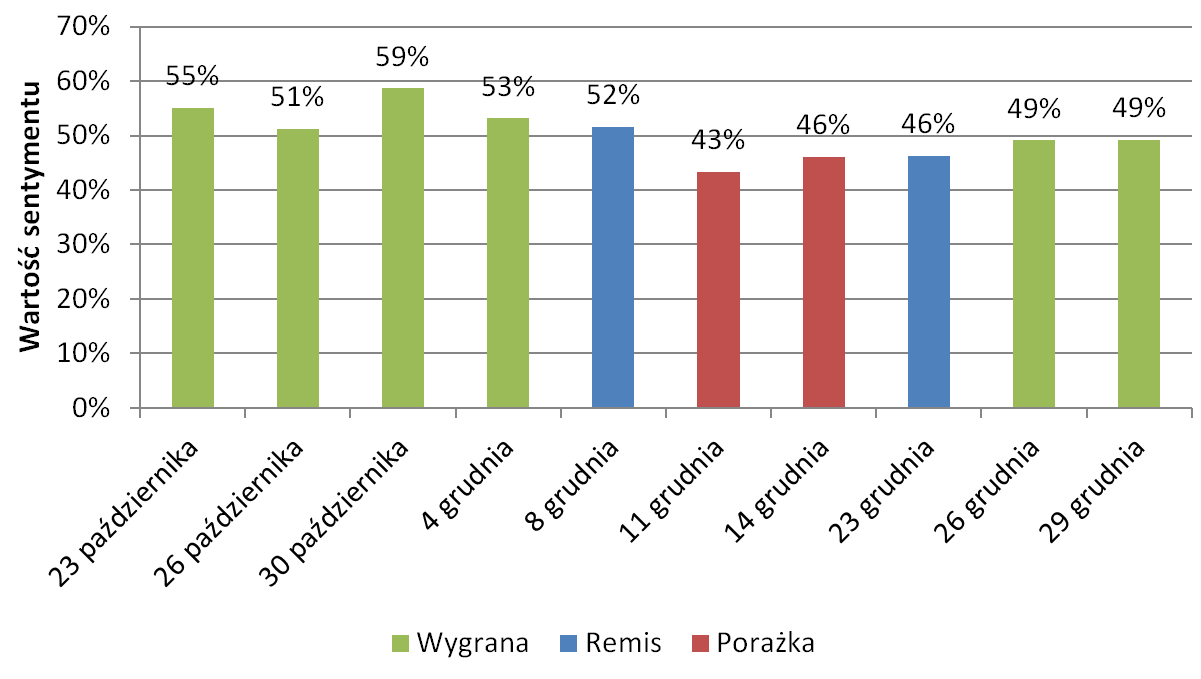
\includegraphics[width=100mm]{img/pozytywnosc-arsenal2.png}
\caption{Wyniki spotkań Arsenalu a sentyment wpisów}
\label{image:pozytywnosc-arsenal}
\end{figure}

\begin{figure}[ht!]
\centering
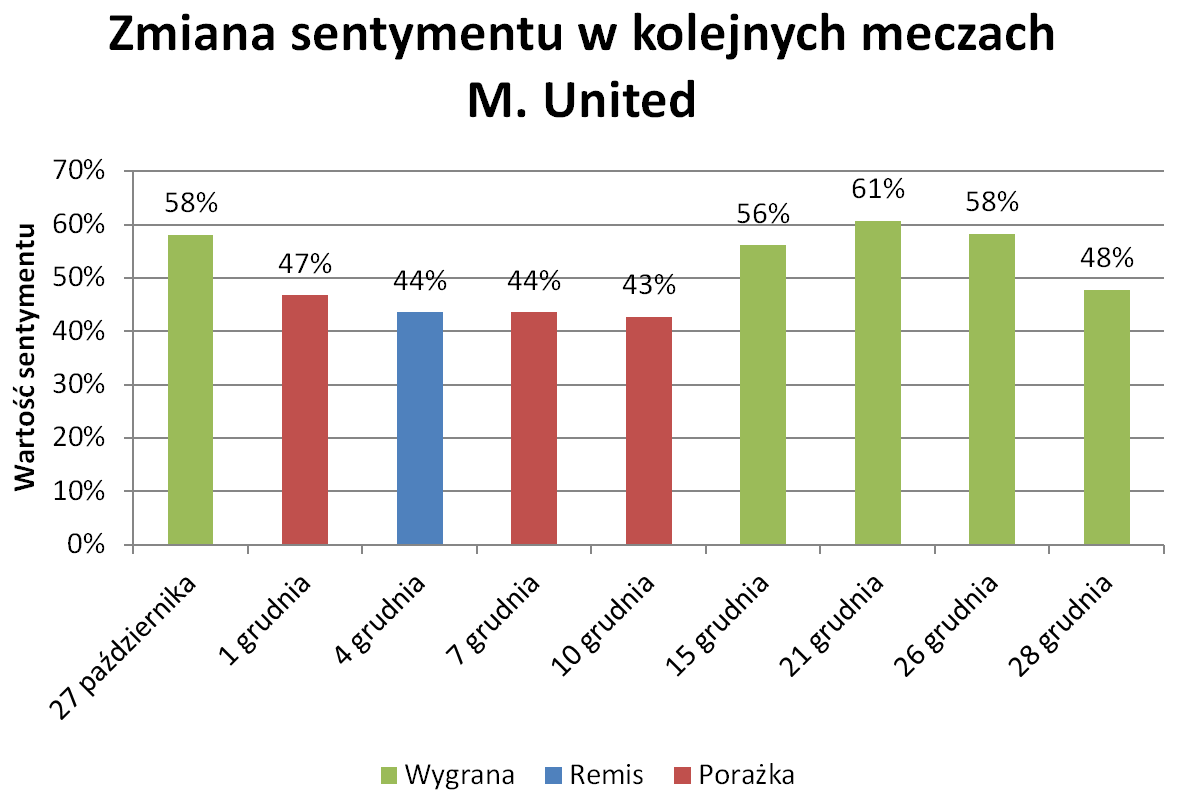
\includegraphics[width=100mm]{img/pozytywnosc-munited2.png}
\caption{Wyniki spotkań Manchesteru United a sentyment wpisów}
\label{image:pozytywnosc-munited}
\end{figure}

Posiadając informację na temat końcowego wyniku danego meczu łatwo można 
zauważyć, iż wartość sentymentu jest adekwatna do uzyskanego rezultatu danej 
drużyny. Gdy Arsenal odnosi zwycięstwo wówczas wpisy mają częściej wydźwięk
pozytywny przekraczając w większości przypadków wartość 50\%. Gdy jednak 
drużyna przegrywa nacechowanie emocjonalne wpisów wyraźnie spada poniżej 46\%.
Również mecz zakończony remisem powoduje raczej wpisy niezadowolenia.
 
Tę samą prawidłowość można zauważyć analizując wyniki badań dla meczów
Manchesteru United. Gdy drużyna wygrywa, wówczas zadowolenia we wpisach sięga
nawet 61\%, a gdy ponosi porażkę -- wynik sentymentu spada do czterdziestu kilku
procent.

Po analizie tych badań nasuwają się oczywiste wnioski. Sposób reagowania
internautów na wyniki ich drużyn jest dokładnie taki sam jak rezultat przez nie
osiągany. Gdy drużyna wygrywa, jej kibice wykazują radość, szczęście,
zadowolenie i inne pozytywne emocje.
Natomiast gdy klub przegrywa mecz, wówczas wśród tweetów dużo łatwiej o wpisy o
nacechowaniu negatywnym. Widać więc, że reakcje użytkowników Twittera są
dokładnie takie same jak zwykłych kibiców -- odzwierciedlają ich aktualny stan
ducha po meczu ulubionej drużyny. Nie ma tutaj żadnej różnicy między światem
realnym a wirtualnym.















\subsection{Liczba tweetów i rozkład sentymentu w ciągu meczu}
\label{subsection:aktywnoscwmeczu}
Kolejnym eksperymentem było zbadanie aktywności użytkowników Twittera w związku
z wydarzeniami na boisku. Badanie takie można przeprowadzić dla każdego meczu,
który znalazł się pośrod tych, które zostały pobrane. Poniżej przedstawione są
rezultaty dla spotkania pomiędzy drużynami Chelsea F.C. a Southampton F.C.
(01.12.2013 r.), które zakończyło się wynikiem 3-1. Są to dwa wykresy: pierwszy
z liczbą tweetów na minutę (z uwzględnieniem wyrażanego przez nie sentymentu) 
\refimg{image:tweety-w-meczu} oraz drugi pokazujący zmianę sentymentu w trakcie
spotkania \refimg{image:sentyment-w-meczu}.

Na obu wykresach zaznaczone są kluczowe wydarzenia:

\begin{enumerate}
  \item \textbf{17:10} -- 1 min., początek meczu i gol J. Rodriguez (Southampton FC) 0-1.
  \item \textbf{17:59} -- 45 + 4 min., koniec pierwszej połowy.
  \item \textbf{18:14} -- 45 min., początek drugiej połowy.
  \item \textbf{18:24} -- 55 min., gol G. Cahill (Chelsea FC) 1-1.
  \item \textbf{18:31} -- 62 min., gol J. Terry (Chelsea FC) 2-1.
  \item \textbf{18:59} -- 90 min., gol D. Ba (Chelsea FC) 3-1.
  \item \textbf{19:05} -- 90 + 6 min., koniec spotkania.
\end{enumerate}



\begin{figure}[ht!]
\centering
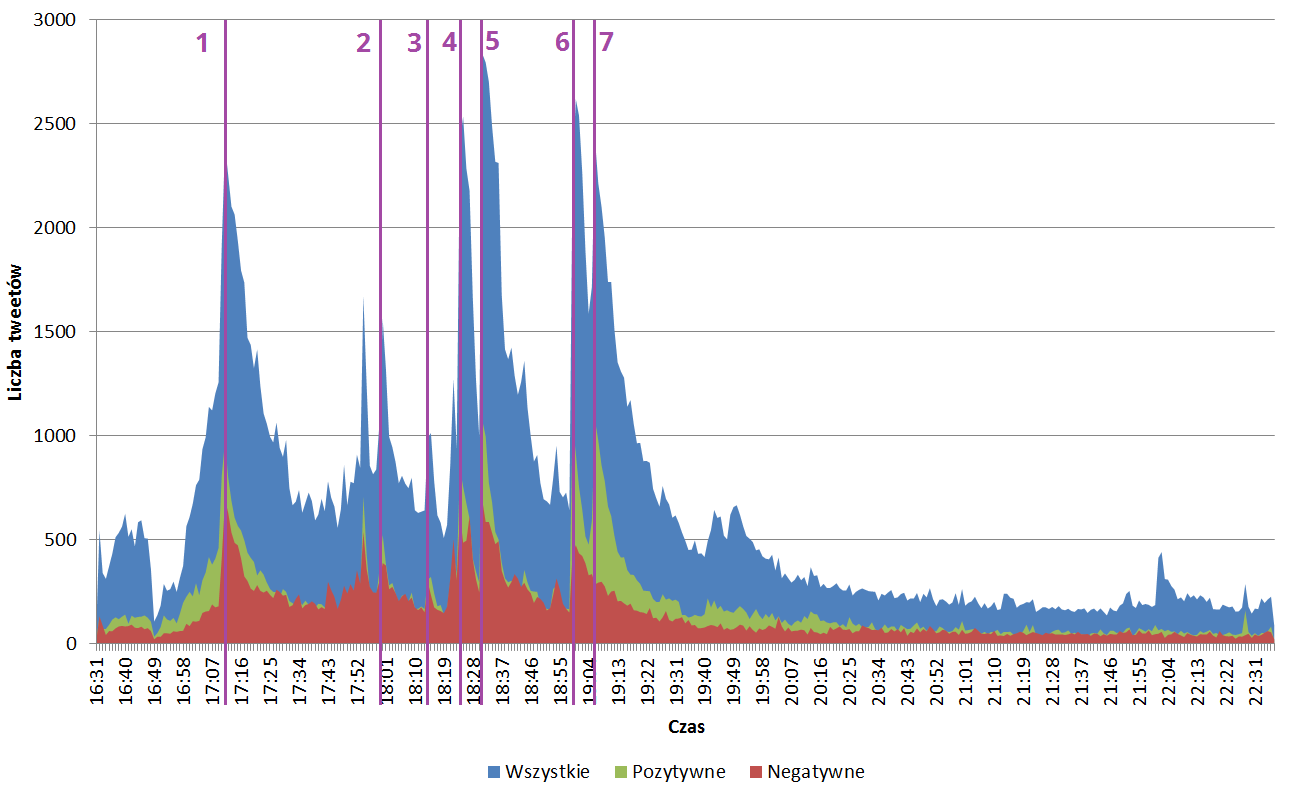
\includegraphics[width=160mm]{img/tweety-w-meczu-nums.png}
\caption{Zmiana liczby tweetów w trakcie meczu Chelsea -- Southampton}
\label{image:tweety-w-meczu}
\end{figure}

\begin{figure}[ht!]
\centering
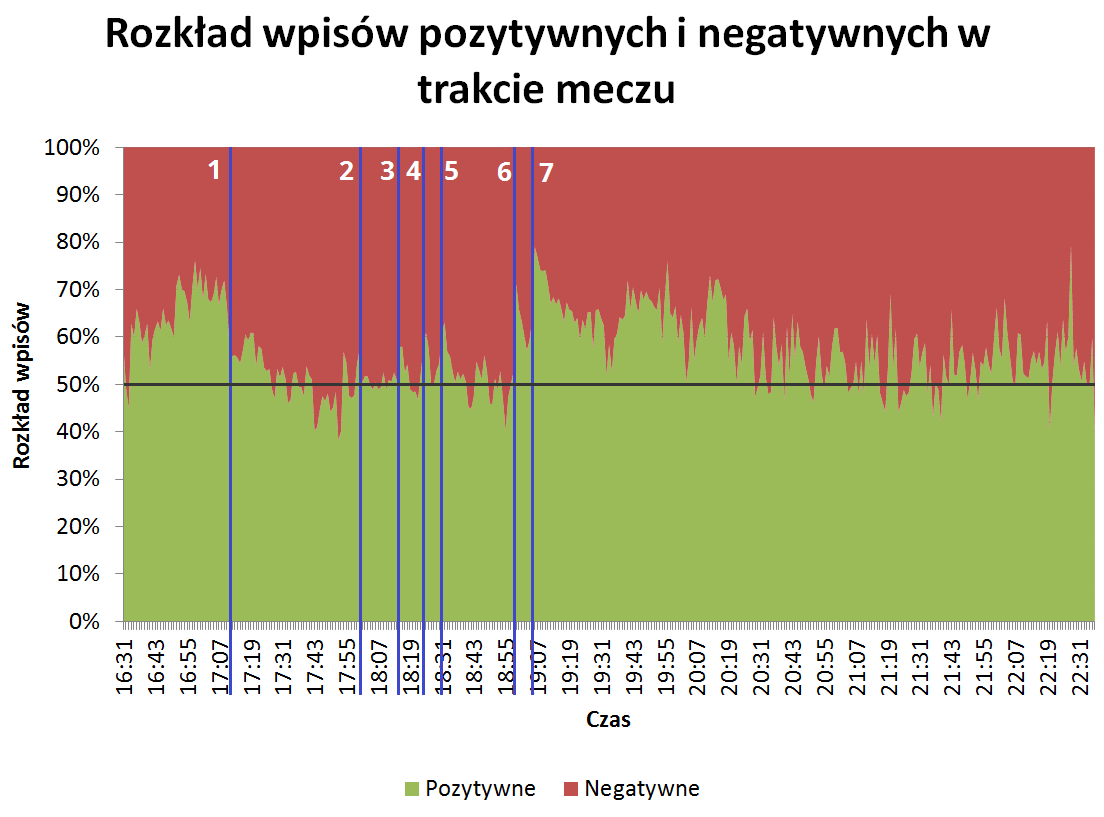
\includegraphics[width=120mm]{img/sentyment-w-meczu-nums-50percentage.png}
\caption{Rozkład sentymentu tweetów w trakcie meczu Chelsea -- Southampton}
\label{image:sentyment-w-meczu}
\end{figure}


Na pierwszym załączonym wykresie \refimg{image:tweety-w-meczu} wyraźnie widać
silną korelację istotnych wydarzeń boiskowych z wysokim wzrostem liczby wysyłanych tweetów. 
Liczba ta rośnie nawet trzykrotnie w przypadku strzelonej bramki przez jedną
z drużyn. Użytkownicy Twittera dużo mocniej angażują się w komentowanie i 
komunikację poprzez to medium w najważniejszych momentach danego spotkania.
Można zauważyć, że początek i koniec spotkania są momentami, w których
kibice generują stosunkowo dużą liczbę wpisów. W trakcie spotkania
ich aktywność wzrasta, gdy na boisku dzieje się coś ciekawego.
Po zakończonym meczu liczba wpisów stopniowo maleje, a dane spotkanie
nie cieszy się już zainteresowaniem takiego szerokiego grona
odbiorców jak wcześniej. Są to już zapewne raczej wiadomości wysyłane
przez bardziej zagorzałych fanów, analizujących dane spotkanie dłużej,
wyciągających z niego wnioski a nie tych osób, które były zainteresowane
meczem tylko wtedy gdy ten się jeszcze odbywał.

Drugi wykres \refimg{image:sentyment-w-meczu} przedstawiający zmiany sentymentu
wyraźnie pokazuje, że wpisy były wyrównane w trakcie meczu (jeśli chodzi o proporcje sentymentu) aż do momentu,
w którym Chelsea FC zdobyła bramkę na 3-1, ustalając w ten sposób de facto
końcowy wynik spotkania. Wówczas wyraźnie przeważały wpisy o wydźwięku
pozytywnym. Sam fakt tego, że to właśnie te tweety były liczniejsze może wynikać
między innymi z tego, że Chelsea to klub mający więcej fanów na całym świecie
niż Southampton, grający w ostatnich latach regularnie w Lidze Mistrzów, bijący
się o zwycięsto w Premier League, czy jeżdżący w trakcie przygotowań do sezonu
na tournee do Stanów Zjednoczonych i Azji. Southampton natomiast to klub z dolnej
części tabeli, mający zupełnie inne cele w trakcie sezonu, nieposiadający tylu
gwiazd, w związku z czym nie skupiający wokół siebie takiego zainteresowania.

Bardzo podobne wykresy można uzyskać analizując także inne spotkania.
Tam również internauci mocniej angażują się, gdy dzieje się coś ciekawego, a
sentyment jest zgodny z wynikiem i liczbą przeważających kibiców danego klubu.
Widać więc, że Twitter jest miejscem, w którym jego użytkownicy uzewnętrzniają
swoje emocje błyskawicznie, gdy dzieje się coś co ich porusza.
Są to takie same naturalne emocje, których doświadczają oni na co dzień, nie są
w żaden sposób wyimaginowane, przemyślane, czy sterowane, ale pokazują aktualny
stan ducha danej społeczności. Można więc dojść do wniosku, że badanie Twittera
może przynieść nam wyniki, do których powinniśmy podejść poważnie i nie
bagatelizować ich twierdząc, że być może w internecie osoby zachowują się
inaczej niż w codziennym życiu.




%%%%%%%%%%%%%%%%%%%%%%%%%%%%%%%%%%%%%%%%%%%%%%%%%%%%%%%%%%%%%% ANALIZA SPOŁECZNA

\section{Analiza sieci społecznych}
\label{section:analizaspoleczna}
Do analizy sieci społecznych zostały użyte dane użytkowników pobrane 
równocześnie ze ściąganiem wpisów. Relacje między użytkownikami zostały
zbudowane na podstawie informacji zawartych w tweetach. Są to więc
dwa rodzaje relacji -- odpowiedzi i retweety. Z ich pomocą przeprowadzone
zostały badania nad siecią społeczną, którą tworzą użytkownicy Twittera. 






\subsection{Liczba i rodzaje komunikacji między zwolennikami i przeciwnikami klubów}
\label{subsection:rodzajekomunikacji}
% retweety pozytywne zwolennicy, replies negatywne, przeciwnicy, itd

Jednym z eksperymentów przeprowadzonych w analizie sieci społecznych było
sprawdzenie rodzaju komunikacji pomiędzy użytkownikami. 
Dodatkowo użytkownicy zostali podzieleni na zwolenników i przeciwników danego 
klubu zgodnie z opisem w rozdziale \ref{subsubsection:wykrywaniezwolennikow}.


\subsubsection{Charakterystyka komunikacji poprzez odpowiedzi (\textit{replies})}
Zbadana został sposób w jaki komunikują się użytkownicy Twittera korzystając
z funkcji \textit{odpowiedz}, polegającej na możliwości komentowania wpisów
innych użytkowników. Tak jak było to wcześniej zaznaczone w tym serwisie
społecznościowym użytkownicy do woli mogą komentować wpisy osób, których
nie mają na swoich listach znajomych.

Poprzez podzielenie użytkowników na grupy zwolenników i przeciwników -- na
przykładzie wpisów dotyczących Manchesteru United -- można zauważyć ciekawe
obserwacje, co można zaobserwować na wykresie \refimg{image:replies-munited}.

\begin{figure}[ht!]
\centering
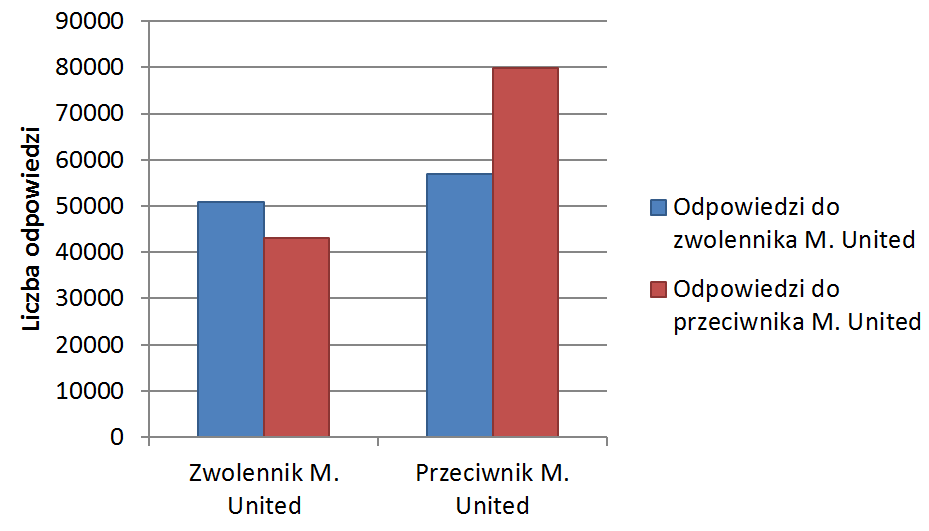
\includegraphics[width=100mm]{img/replies-munited.png}
\caption{Charakterystyka odpowiedzi wśród wpisów dotyczących Manchesteru United}
\label{image:replies-munited}
\end{figure}

Wykres przedstawia liczbę odpowiedzi zwolenników i przeciwników Manchesteru 
United na wpisy zwolenników i przeciwników tego klubu. Na jego podstawie można
zauważyć, że na wpisy zwolenników częściej odpowiadają zwolennicy. 
Oznacza to, że ta grupa użytkowników trzyma się blisko siebie i osoby, które
są sympatykami Manchesteru również obserwują i komunikują się z innymi 
sympatykami tego klubu produkując większą liczbę wpisów.
Podobna zależność ma miejsce wśród przeciwników Manchesteru United.
Wpis przeciwnika tego klubu bardziej angażuje do dyskusji również innych
przeciwników. Prawdopodobnie osoby biorące udział w tej dyskusji wspólnie
narzekają na grę tego zespołu, wzajemnie nakręcając się do ożywionych dyskusji.

Na podstawie powyższego wykresu widać więc, że użytkownicy Twittera lubią 
tworzyć grupy o podobnych zainteresowaniach czy sympatiach. Dany użytkownik
częściej będzie komunikował się z osobami, które myślą podobnie jak on,
umacniając w ten sposób swoje przekonanie o własnych przemyśleniach na dany temat.
Gdy ktoś jest zwolennikiem danego klubu częściej dyskutuje z podobnymi sobie
internautami. Tak samo przeciwnicy łatwiej znajdują nić porozumienia między sobą
mając takie samo zdanie dotyczące określonego wydarzenia. Internauci lepiej
odnajdują się wśród osób podzielających ich opinie.  









\subsubsection{Charakterystyka komunikacji poprzez retweety}
Podobnie jak powyższe badanie został przeprowadzony eksperyment na temat 
charakterystyki komunikacji między użytkownikami korzystający z opcji 
\textit{retweet}. Polega ona na podaniu dalej wpisu, który uważamy za ciekawy.
Wyniki, które w ten sposób uzyskano różnią się od poprzednich
\refimg{image:retweety-munited}.

\begin{figure}[ht!]
\centering
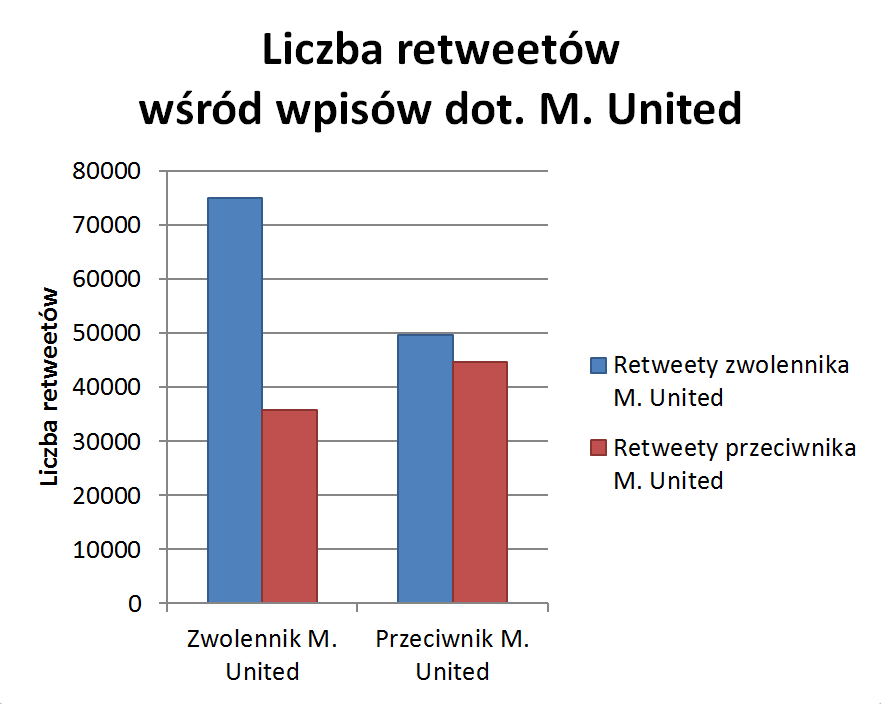
\includegraphics[width=100mm]{img/retweety-munited.png}
\caption{Charakterystyka retweetów wśród wpisów dotyczących Manchesteru United}
\label{image:retweety-munited}
\end{figure}


Tym razem widać zupełnie inne ułożenie słupków na wykresie (rys.
\ref{image:replies-munited} i \ref{image:retweety-munited}).
Na pierwszy plan wyraźnie wysuwa się słupek pierwszy z lewej, który oznacza
liczbę wpisów zwolenników podanych dalej przez innych zwolenników. Widać więc,
że sympatycy Manchesteru United bardzo chętnie przekazują dalej wpisy 
pozostałych sympatyków. Mogą to być na przykład wpisy o strzelonym golu,
czy jakieś pozytywne opinie na temat danej drużyny. Najrzadziej z całej
czwórki zaprezentowanych relacji dochodzi do sytuacji, gdy przeciwnik
Manchseteru podaje dalej wpis zwolennika. Jeśli chodzi o retweetowanie
tweetów przeciwników Manchesteru United, to dochodzi do tego mniej więcej po
równo między przeciwnikami i zwolennikami.

Po analizie dwóch powyższych eksperymentów nasuwają się następujące wnioski.
Użytkownicy lubią gromadzić się w grupy o podobnych zainteresowaniach,
wspólnie komentując wydarzenia w podobny sposób. Zwolennicy i przeciwnicy
danego klubu zachowują się w charakterystyczny sposób. Ci pierwsi bardzo często
retweetują wpisy innych zwolenników, a ci drudzy częściej dyskutują ze sobą.




\subsection{Sentyment odpowiedzi między zwolennikami i przeciwnikami drużyny}
\label{subsection:sentymentwrelacjach}
Oprócz zbadania rodzaju i charakterystyki komunikacji pomiędzy użytkownikami 
Twittera przyjrzano się także bliżej komunikacji związanej z odpowiedziami 
(\textit{replies}). Przeprowadzono eksperyment, w którym zwrócono uwagę
na wydźwięk wpisów będących odpowiedziami na inne wpisy -- ponownie z podziałem
na zwolenników i przeciwników danej drużyny. W tym rozdziale skupiono się tylko
na odpowiedziach, gdyż niemożliwe jest badanie sentymentu retweetów, które są
tylko podaniem dalej innych wpisów. Poniżej prezentuję jak rozkładał się
sentyment wpisów dla wszystkich kombinacji zwolenników i przeciwników
Arsenalu jako autorów i odpowiadających.


\subsubsection{Gdy odpowiada zwolennik Arsenalu}
Poniżej prezentuję dwie sytuacje, w których odpowiadającym na wpis jest
użytkownik będący zwolennikiem drużyny Arsenalu Londyn. W pierwszym przypadku
\refimg{image:reply-sentiment-zwolennik-zwolennik} pokazana jest struktura
odpowiedzi zwolennika na wpisy innego zwolennika, zaś w drugim
\refimg{image:reply-sentiment-zwolennik-przeciwnik} odpowiedzi odnoszą się do
wpisów przeciwnika klubu.

\begin{figure}[ht!]
\centering
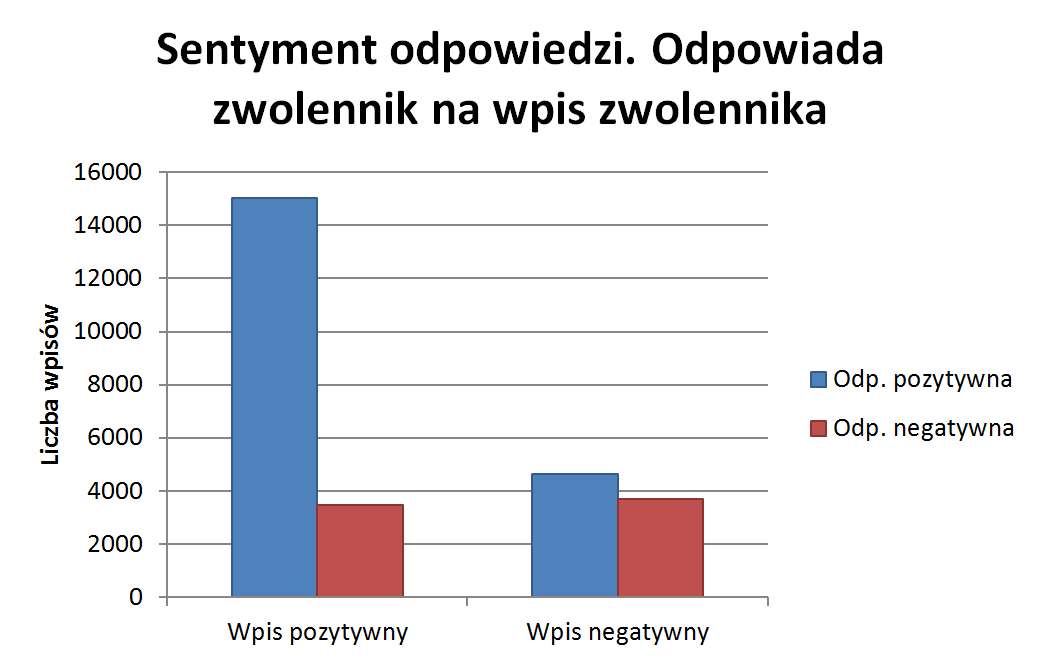
\includegraphics[width=100mm]{img/reply-sentiment-zwolennik-zwolennik.png}
\caption{Sentyment odpowiedzi. Odpowiada zwolennik Arsenalu na wpis zwolennika}
\label{image:reply-sentiment-zwolennik-zwolennik}
\end{figure}


\begin{figure}[ht!]
\centering
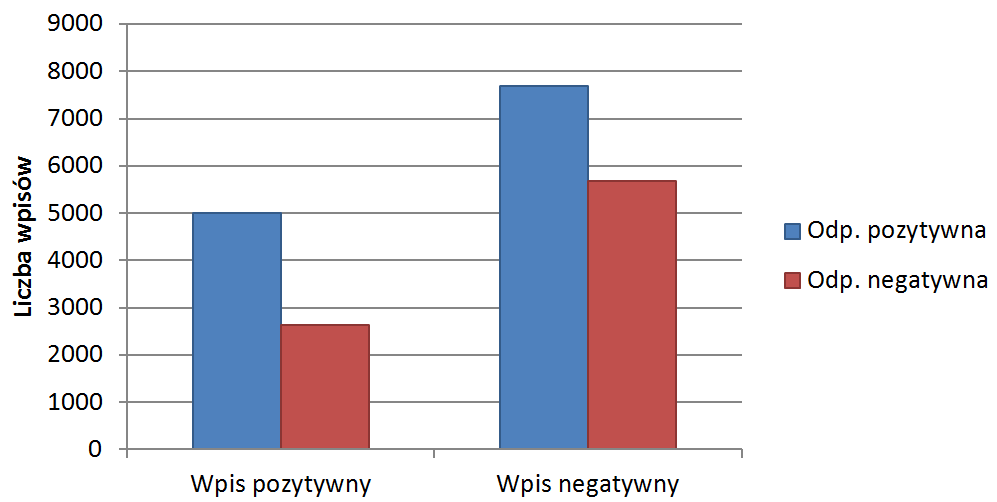
\includegraphics[width=100mm]{img/reply-sentiment-zwolennik-przeciwnik.png}
\caption{Sentyment odpowiedzi. Odpowiada zwolennik Arsenalu na wpis przeciwnika}
\label{image:reply-sentiment-zwolennik-przeciwnik}
\end{figure}



To co rzuca się na pierwszy rzut oka to fakt, że 
zwolennicy danego klubu najczęściej tworzą wpisy pozytywne. Zauważalne jest to,
że wśród zwolenników dominującym modelem komunikacji jest wymiana wiadomości
o nacechowaniu pozytywnym -- na wpis pozytywny odpowiedzą jest również wpis o 
takim samym sentymencie -- wyraźnie wyróżniająca się spośród pozostałych
wariantów.
Zauważyć można również to, że przeciwnicy Arsenalu generują więcej wpisów 
negatywnych a mimo to sympatycy klubu z Londynu starają się im odpowiadać
tweetami o wydźwięku pozytywnym.

Widać więc, że osoby tworzące pozytywne wpisy na dany temat pobudzają się
wzajemnie do ożywionej dyskusji a także starają się dbać o dobre imię
i dobry odbiór tematu, który jest im bliski. Tworzą więc grupę, która
dobrze czuje się w swoim towarzystwie a także stara się kreować
pozytywny odbiór swojego ulubionego klubu na zewnątrz, wśród innych osób.

\subsubsection{Gdy odpowiada przeciwnik Arsenalu}
Analogicznie do poprzednich eksperymentów w dwóch wykresach poniżej (na 
rysunkach \ref{image:reply-sentiment-przeciwnik-zwolennik} i 
\ref{image:reply-sentiment-przeciwnik-przeciwnik}) zaprezentowane są
wyniki badań nad odpowiedziami przeciwnika Arsenalu na wpisy zwolenników
i przeciwników tego klubu.

\begin{figure}[ht!] \centering
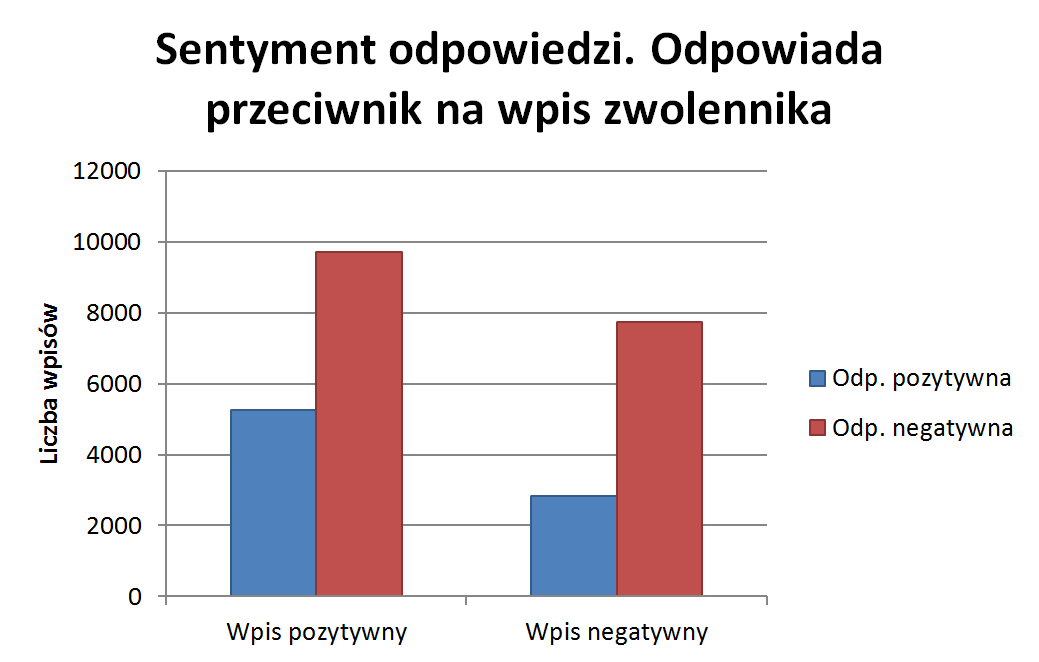
\includegraphics[width=100mm]{img/reply-sentiment-przeciwnik-zwolennik.png}
\caption{Sentyment odpowiedzi. Odpowiada przeciwnik Arsenalu na wpis zwolennika}
\label{image:reply-sentiment-przeciwnik-zwolennik}
\end{figure}

\begin{figure}[ht!] \centering
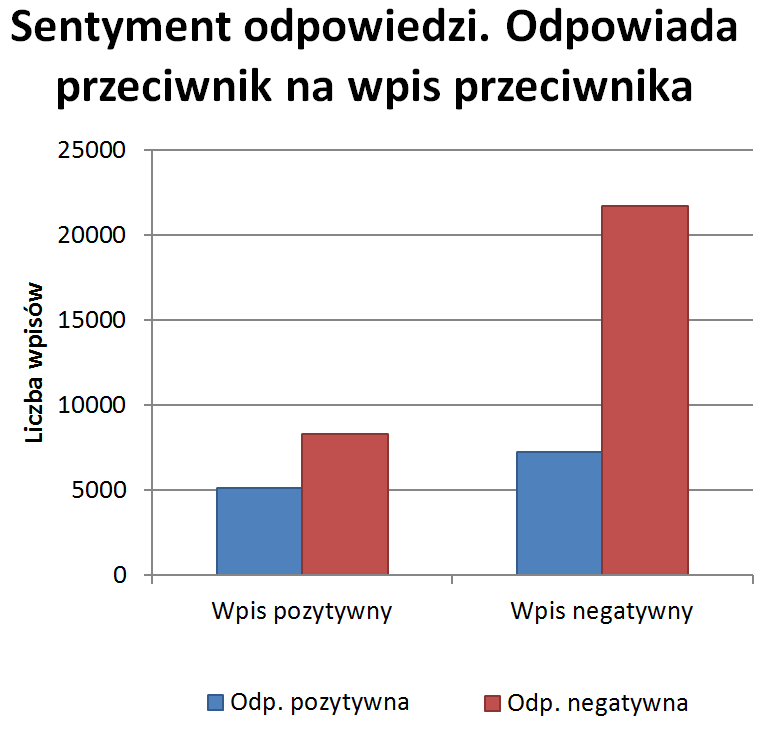
\includegraphics[width=100mm]{img/reply-sentiment-przeciwnik-przeciwnik.png}
\caption{Sentyment odpowiedzi. Odpowiada przeciwnik Arsenalu na wpis przeciwnika}
\label{image:reply-sentiment-przeciwnik-przeciwnik}
\end{figure}

Z powyższych wykresów można wywnioskować, że wpisy przeciwników mają najczęściej
wydźwięk negatywny. Gdy przeciwnik odpowiada na pozytywny wpis zwolennika, to tylko
1 na 3 wpisy są również pozytywne. Zdecydowanie częściej przeciwnik odpisuje
zwolennikowi wpisem o sentymencie negatywnym. 
Co warte zauważenia najwięcej odpowiedzi przeciwnicy Arsenalu wysyłają
pod wpisami negatywnymi innych przeciwników, również nacechowując swoje opinie
negatywnie.

Analogicznie więc jak w poprzednim eksperymencie widać, że przeciwnicy
Arsenalu tworzą wspólną grupę, w której wymieniają się swoimi
krytycznymi opiniami na temat tej drużyny. I tak samo jak poprzednio
wychodzą również z tymi opiniami do innych internautów starając się
przekonać ich do swojego punktu widzenia.
















%%%%%%%%%%%%%%%%%%%%%%%%%%%%%%%%%%%%%%%%%%% ANALIZA GRUP W SIECIACH SPOŁECZNYCH
\subsection{Analiza grup w sieciach społecznych}
\label{subsection:strukturagrup}
Oprócz powyższych badań nad sposobami komunikacji i relacji budowanymi między
użytkownikami przeprowadzona została także analiza grup użytkowników 
pomiędzy meczami. Grupy te były budowane zgodnie z
opisem w rozdziale \ref{subsubsection:koncepcja-wykrywaniegrup}.

Liczności tych grup zostało zaprezentowane na poniższych
wykresach pokazując jak zmieniały się z meczu na mecz.
Na pierwszym \refimg{image:grupy-arsenal} przedstawione są dane
dla Arsenalu, a na drugim \refimg{image:grupy-munited} dla Manchesteru United.
Oprócz wielkości poszczególnych grup wykresy prezentują także podobieństwo
zbioru użytkowników komentującego następujące po sobie wydarzenia.
Sposoby wykrywania grup i badania podobieństwa zostały opisane w rozdziale
\ref{subsection:miary-relacje}.
 
\begin{figure}[ht!]
\centering
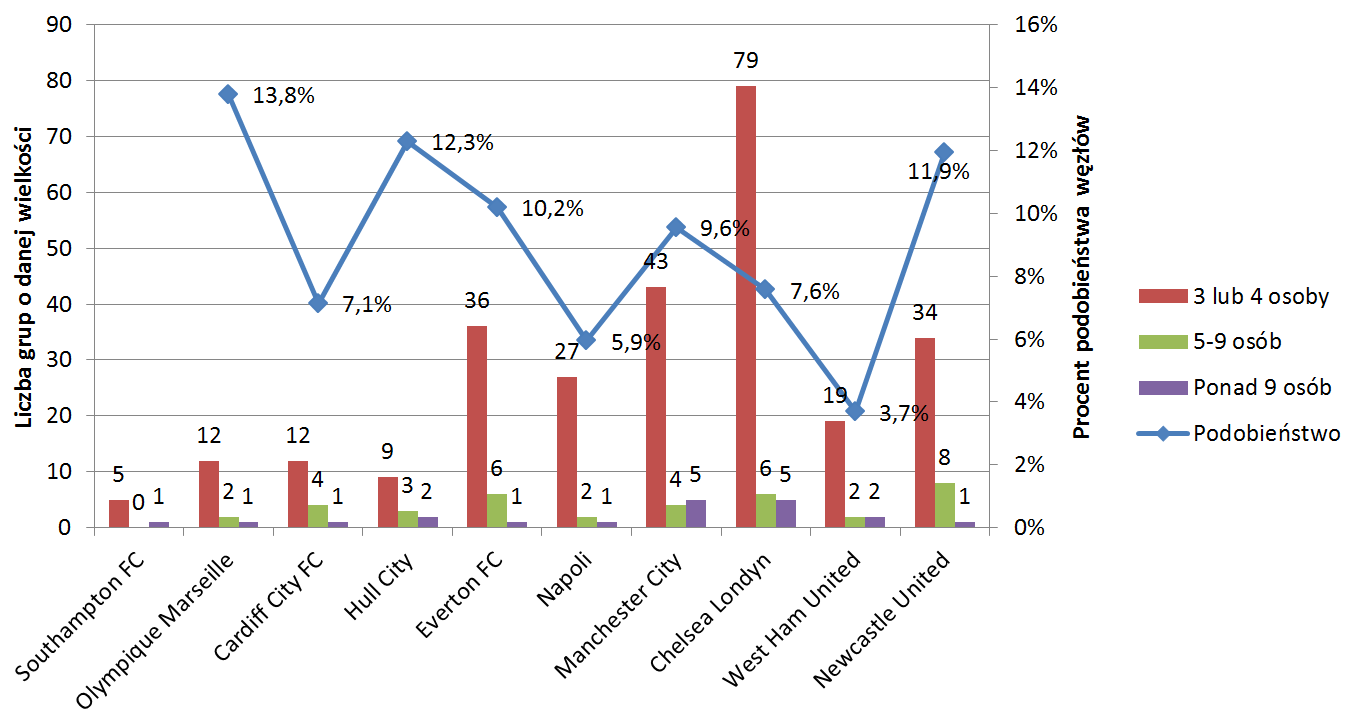
\includegraphics[width=160mm]{img/grupy-arsenal-nums.png}
\caption{Struktura grup użytkowników w meczach Arsenalu}
\label{image:grupy-arsenal}
\end{figure}

\begin{figure}[ht!]
\centering
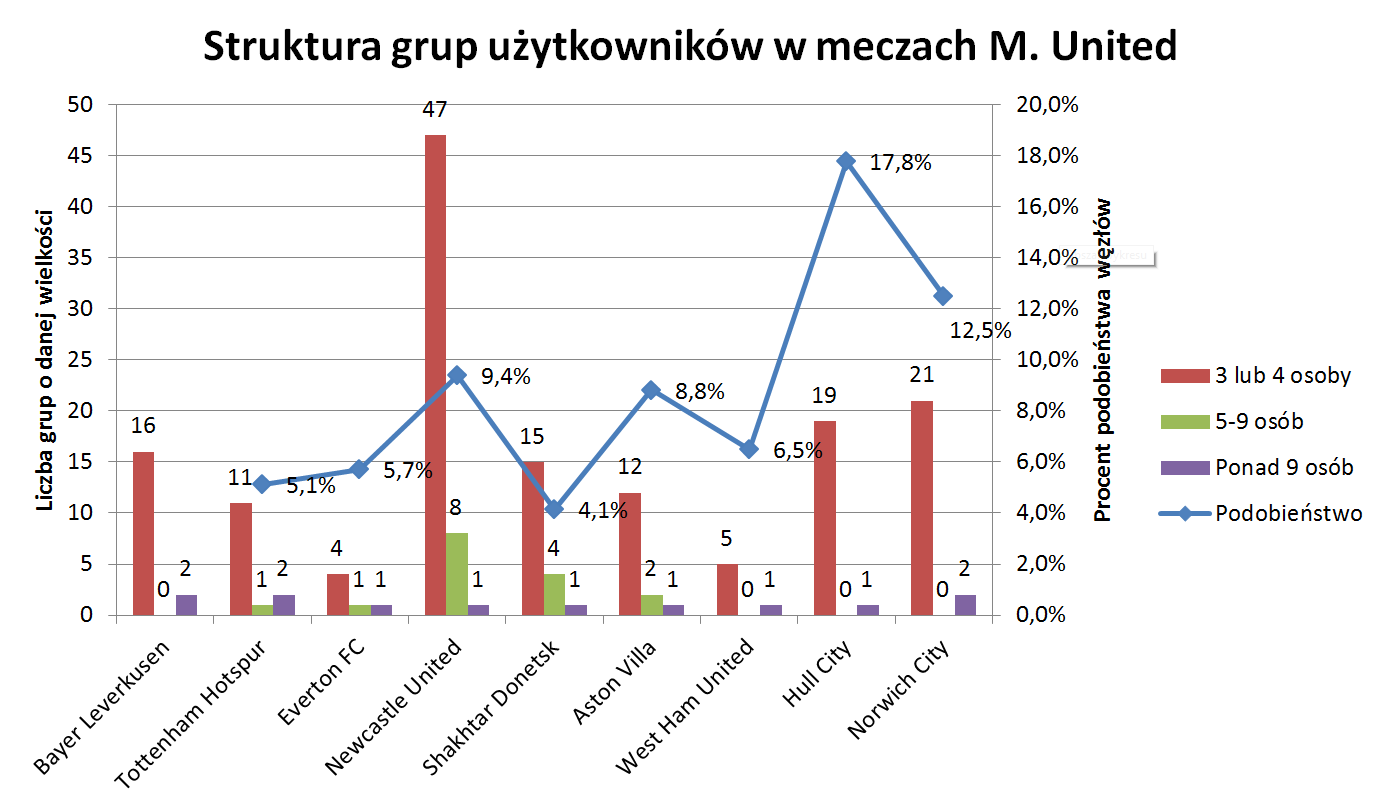
\includegraphics[width=160mm]{img/grupy-munited-nums.png}
\caption{Struktura grup użytkowników w meczach Manchesteru United}
\label{image:grupy-munited}
\end{figure}


Z analizy wykresów można zaobserwować, że w każdym spotkaniu najliczniejsze
są małe grupy -- 3 lub 4 osobowe. Liczba tych grup dodatkowo rośnie gdy
mecz odbywa się z ciekawym przeciwnikiem. Na przykład zauważyć można, że
w meczach Arsenalu \refimg{image:grupy-arsenal} bardzo dużą liczbę grup wygenerowały
spotkania z Manchesterm Citym i Chelsea Londyn, a w meczach Manchesteru United
skok liczby grup miał miejsce w meczu z Newcastle United.
Grupy liczniejsze jeśli chodzi o wielkość tworzyły się już zdecydowanie rzadziej.
I podobnie jak poprzednio ich większa liczbę również można zaobserwować
w ciekawszych spotkaniach.

Jeśli zaś chodzi o podobieństwo w kolejnych meczach to mamy tutaj do czynienia
z ciekawą, aczkolwiek zrozumiała sytuacją. Otóż im ciekawszy przeciwnik,
tym podobieństwo zbioru użytkowników w kolejnym meczu mniejsze.
Gdy drużyna -- w przypadku Arsenalu --  gra najpierw z Chelsea a później z 
West Ham United, to podobieństwo wynosi 3.7\%, a gdy najpierw gra z 
West Ham United -- w przypadku Manchesteru Untied -- a potem z Hull City
to podobieństwo między tymi meczami sięga 17.8\%.

Widać więc pewną charakterystyczną zależność. Gdy drużyna gra mecze z popularnymi
drużynami, wówczas liczba osób biorących na Twitterze udział w danym wydarzeniu
piłkarskim jest duża. Spotkanie takie absorbuje większą publikę. Stąd
większe słupki grup w popularnych meczach. Gdy jednak przeciwnik jest już nieco
mniej ciekawy, wówczas również zainteresowanie na Twitterze takim meczem spada.

Z tych prawidłowości wynika również dlaczego osiągany był taki a nie inny
wynik podobieństwa. Otóż gdy zespół gra mecz. to zawsze
wśród tweetujących na jego temat jest stała grupa fanów, która w spotkaniach
ze słabymi rywalami jest łatwiej dostrzegalna -- stanowi większy odsetek
wszystkich użytkowników Twittera. Gdy natomiast mecz jest interesujący
dla większej liczby odbiorców -- wówczas ta stała grupa fanów jest trudniej
dostrzegalna i odsetek podobieństwa drastycznie spada.
Mecze z ciekawymi rywalami przyciągają więc do siebie osoby okazjonalnie zainteresowane
danym temat -- te osoby następnym razem nie będą komentować meczu tej drużyny,
gdy ta będzie rozgrywać spotkanie z mało ciekawym rywalem. 
Wówczas jednak łatwiej będzie dostrzec tę grupę, która stanowi trzon zainteresowanych
daną drużyną i która jest jej stałym fanem.


% Podobieństwo węzłów między meczami 
% Podobieństwo grafów między meczami 
% Między mało popularnymi spotkaniami wysoki stopień podobieństwa
% +Sentyment a wielkość grupy











%%%%%%%%%%%%%%%%%%%%%%%%%%%%%%%%%%%%%%%%%%%%%%%%%%%%%%%%%% ANALIZA GEOGRAFICZNA

\section{Analiza geolokacji}
\label{section:analizageograficzna}

W moich badaniach skupiłem się także na zachowaniu użytkowników z wykorzystaniem 
o geolokalizację. Tak jak wspomniałem wcześniej, niewielka część wpisów
zawierała informacje o tym, z którego miejsca została wysłana.
Przy ich pomocy możliwe było dokonanie analizy danych związanych z położeniem
geograficznym.

\subsection{Odległość między użytkownikami a częstość kontaktów}
\label{subsection:odlegloscmiedzyuzytkownikami}
Pierwsze badanie polegało na zmierzeniu odległości fizycznej pomiędzy
użytkownikami, którzy się ze sobą kontaktują i zbadaniu korelacji tej odległości
do liczby wiadomości jakie między sobą wymieniają. Sposób przeprowadzenia tego
badania został opisany w rozdziale \ref{subsubsection:zmierzenieodleglosci}.

\begin{figure}[ht!]
\centering
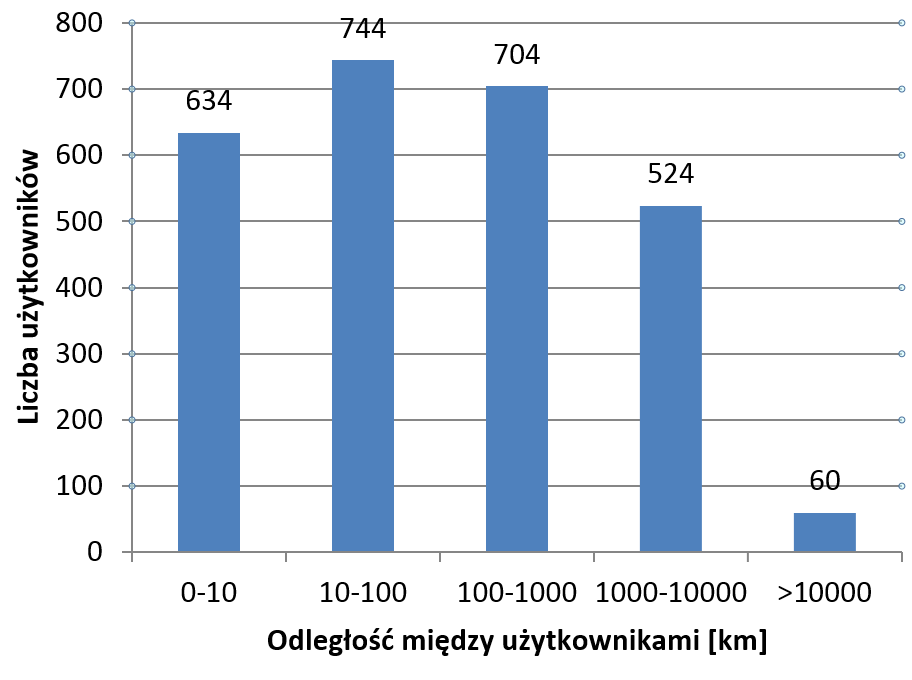
\includegraphics[width=80mm]{img/relacje-a-odleglosc.png}
\caption{Odległość między użytkownikami a częstość kontaktów}
\label{image:relacje-a-odleglosc}
\end{figure}

Każda kolejna kolumna na powyższym wykresie pokrywa obszar o dziesięciokrotnie 
większym promieniu. Oznacza to, że powierzchnia, której dotyczą rośnie
eksponencjalnie. Pomimo tego, liczba użytkowników którzy wchodzili ze sobą
w interakcje jest za każdym razem tego samego rzędu wielkości (co widać na
wykresie \ref{image:relacje-a-odleglosc}).
Oznacza to więc, że im bliżej siebie byli użytkownicy fizycznie tym częściej
odpowiadali na swoje wpisy. Gdy znajdowali się w odległości maksymalnie
10 kilometrów to do wymiany wpisów dochodziło tak samo
często gdy byli od siebie oddaleni od 10 do 100 km, czy nawet od 100 do 1000 km.

Wniosek jest więc taki, iż pomimo tego, że internet nazywany jest globalną wioską
łączącą ludzi z całego świata to użytkownicy komunikują się i tak z najbliższymi
sobie. Może to wynikać z kilku powodów. Na przykład osoby z Manchesteru 
prawdopodobnie będą kibicami drużyny United lub City i większe jest prawdopodobieństwo,
że będą komunikać się między sobą niż między osobami z innego miasta czy kraju.
Innym powodem takiego stanu rzeczy może być również bariera językowa.
Im dalej od danego kraju, tym mniej osób będzie w stanie posługiwać się językiem
tam panującym. Dodatkowym ograniczeniem może być czas lokalny, czyli strefy czasowe.
Gdy w jednym punkcie jest dzień, w drugim może być środek nocy jednoznacznie 
utrudniający komunikację między osobami z większych odległości.  

%Odległość od stadionu zwolenników, przeciwników 
%Odległość od stadionu a sentyment
%Miejscowości a sentyment 
%Kraje, a sentyment


\clearpage
\subsection{Rozkład wpisów na mapie}
\label{subsection:rozkladnamapie}
% Mecz Chelsea - Southampton, 01.12.2013 17:10.
Zebrane Tweety posiadające geolokalizację można przedstawić na
mapie\footnote{Załączone wizualizacje zostały stworzone przy pomocy serwisu
CartoDB (www.cartodb.com)}.
Poniżej na trzech kolejnych rysunkach zaprezentowany został rozkład wpisów,
które wysłane zostały podczas meczu Chelsea F.C. z Southampton F.C.
(01.12.2013 r.). Najpierw zaprezentowane są wpisy w skali całej Ziemii
\refimg{image:mapa-swiata}, następnie w skali Wielkiej Brytanii
\refimg{image:mapa-uk}, a na końcu na mapie zawierającej obszar między Londynem
a Southampton \refimg{image:mapa-uk-zoom}, czyli miastami obu klubów.

\begin{figure}[ht!]
\centering
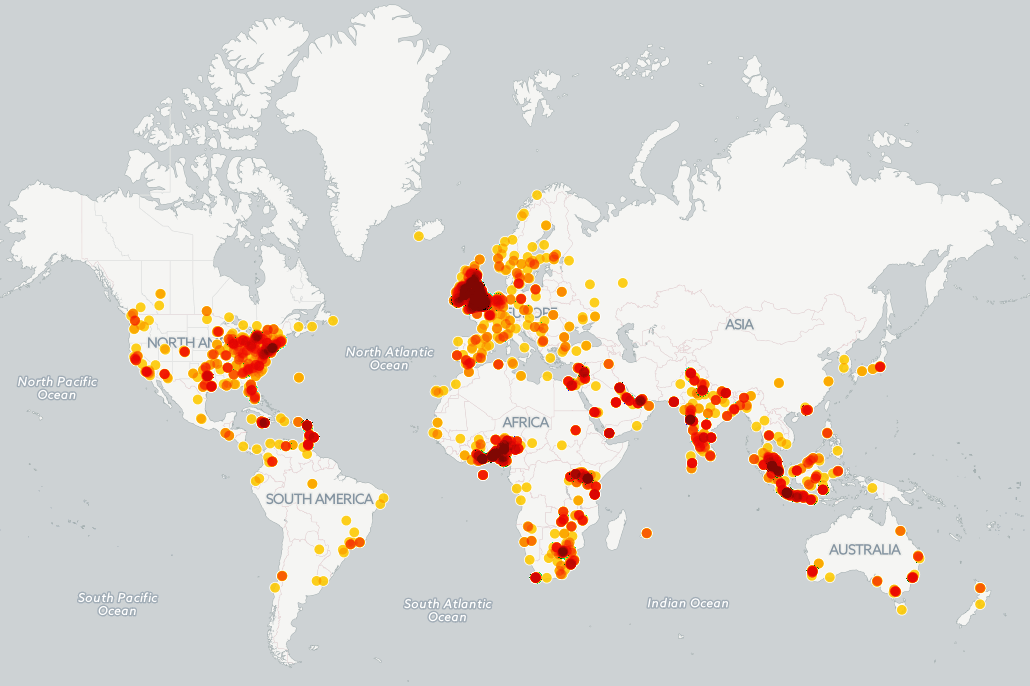
\includegraphics[width=140mm]{img/geo-chelsea-southampton-light.png}
\caption{Rozkład wpisów na mapie świata}
\label{image:mapa-swiata}
\end{figure}

Na mapie świata \refimg{image:mapa-swiata} wyróżnia się kilka krajów. Przede
wszystkim na pierwszym plan wyłania się Wielka Brytania -- z oczywistych względów jako
miejsce, w którym odbywa się mecz oraz całe rozgrywki. Oprócz niej dużą liczbę
tweetów wysyła się z takich krajów jak między innymi:
Stany Zjednoczone (3~kraj pod względem liczby ludności na świecie, dominujący
język angielski), Indie (2~kraj pod względem ludności, język angielski),
Indonezja (4~kraj pod względem ludności) a także państwa afrykańskie: Kenia i Uganda na
wschodze oraz Nigeria i Ghana na zachodzie. Należą one do najbardziej
zaludnionych krajów Czarnego Lądu i w każdym z nich język angielskim jest
językiem urzędowym.
Na mapie nie ma wpisów z Chin (najludniejszego kraju świata gdzie Twitter
został zablokowany w 2009
roku\footnote{http://www.theguardian.com/technology/2009/jun/02/twitter-china})
oraz Rosji, w której popularniejsze są rodzime serwisy społecznościowe.

W meczu wzięli udział między innymi zawodnicy z Nigerii (John Obi Mickel -- Chelsea FC)
oraz Ghany (Michael Essien -- Chelsea FC, Victor Wanyama -- Southampton FC),
co zapewne wzmogło aktywność internautów z tych regionów.


\begin{figure}[ht!]
\centering
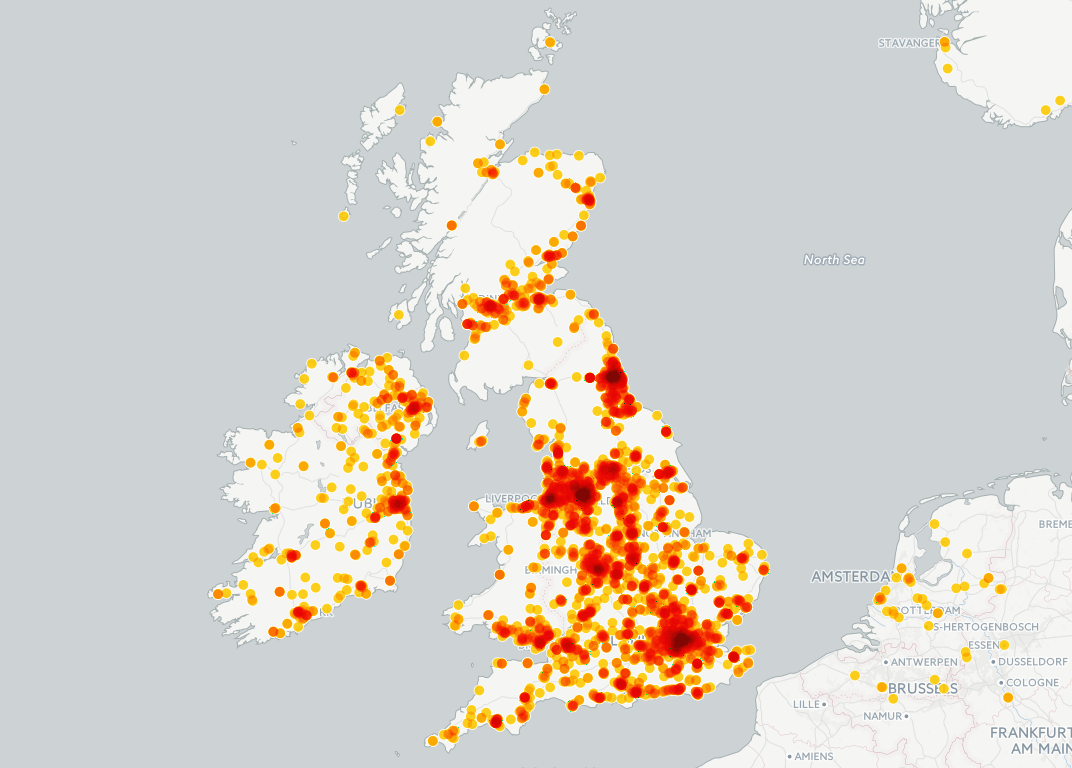
\includegraphics[width=140mm]{img/geo-uk-chelsea-southampton-light.png}
\caption{Rozkład wpisów w Wielkiej Brytani}
\label{image:mapa-uk}
\end{figure}

\begin{figure}[ht!]
\centering
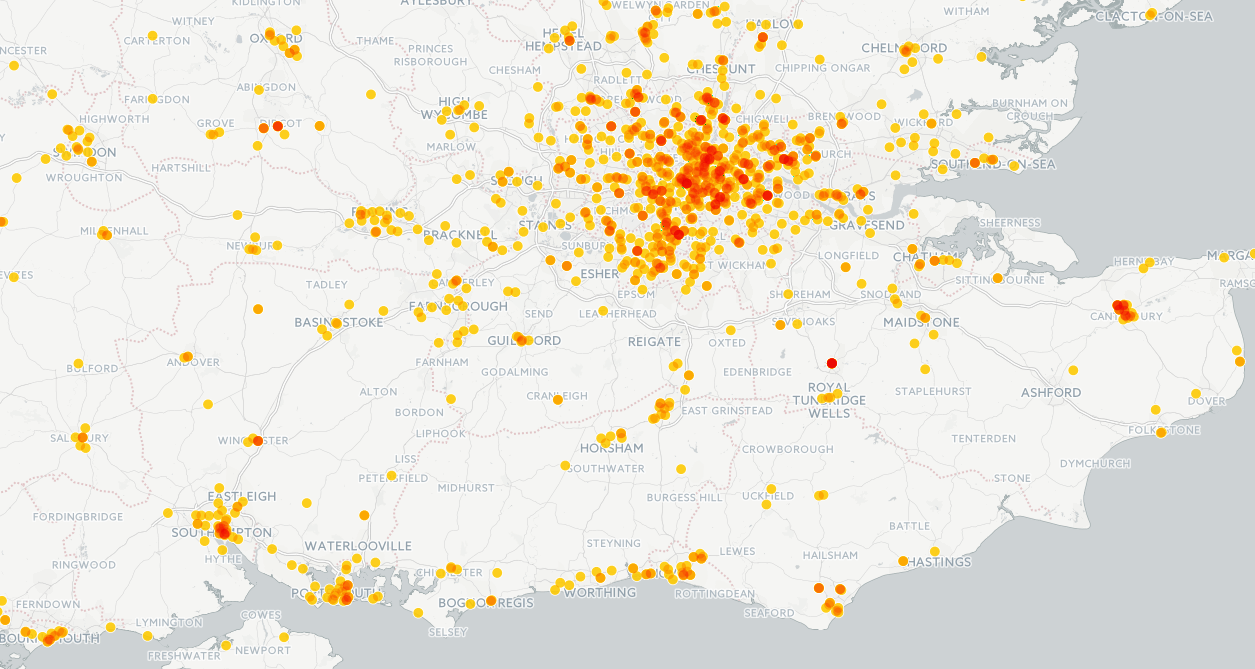
\includegraphics[width=140mm]{img/geo-uk-zoom-chelsea-southampton-light.png}
\caption{Rozkład wpisów wokół Londynu i Southampton}
\label{image:mapa-uk-zoom}
\end{figure}

Oceniając rozkład wpisów w Wielkiej Brytanii \refimg{image:mapa-uk} zauważymy
dużą ich koncetrację wokół Londynu -- największego miasta Zjednoczonego
Królestwa (algomeracja Londynu to ponad 13 milionów ludzi\footnote{2012 rok.
Źródło: Eurostat
(http://appsso.eurostat.ec.europa.eu/nui/show.do?dataset=met\_pjanaggr3\&lang=en)}).
Gdy zbliżymy mapę do obszaru Southampton i Londynu \refimg{image:mapa-uk-zoom}
to za pomocą analizy rozkładu wpisów na mapie bez problemu zlokalizujemy
położenie tych miast.
Właśnie w nich znajduje się najwięcej ich kibiców generujących największą liczbę
wpisów.
Widać więc, że dane wydarzenie angażuje przede wszystkim osoby, którym jest ono
bliskie. Zastosowanie geolokalizacji pozwala nam te miejsca odkryć. I tak jak w
przypadku meczu piłarskiego można takie miejsca określić de facto jeszcze przed
analizą, tak w innego rodzaju badaniach przy użyciu tej techniki możliwe może
być odkrycie miejsc, obszarów geograficznych, o których nie myślałoby się w
kontekście badanego tematu. Powyższe wizualizacje potwierdzają stosowność
zastosowania geolokacji i jej skuteczności w różnego rodzaju badaniach
społecznych.

\subsection{Odległość od stadionu}
\label{subsection:odlegloscodstadionu}
Dane zawierające geolokalizację pozwalają wykonać szereg ciekawych
eksperymentów.
Kolejnym z nich było zbadanie odległości kibiców od stadionu w zależności od
tego czy drużyna grała mecz u siebie czy na wyjeździe. Dodatkowo kibiców tych
(dzięki analizie sentymentu \rref{subsubsection:wykrywaniezwolennikow}) można
było podzielić na zwolenników i przeciwników. Takie badanie zostało
przeprowadzone dla wszystkich meczów Arsenalu Londyn a wyniki zaprezentowane są
na rysunkach \ref{image:odleglosc-od-stadionu-gospodarz} i
\ref{image:odleglosc-od-stadionu-gosc}.
Eksperyment ten został przeprowadzony zgodnie z opisem w rozdziale
\ref{subsubsection:badanieodleglosciodstadionu}.

\begin{figure}[ht!]
\centering
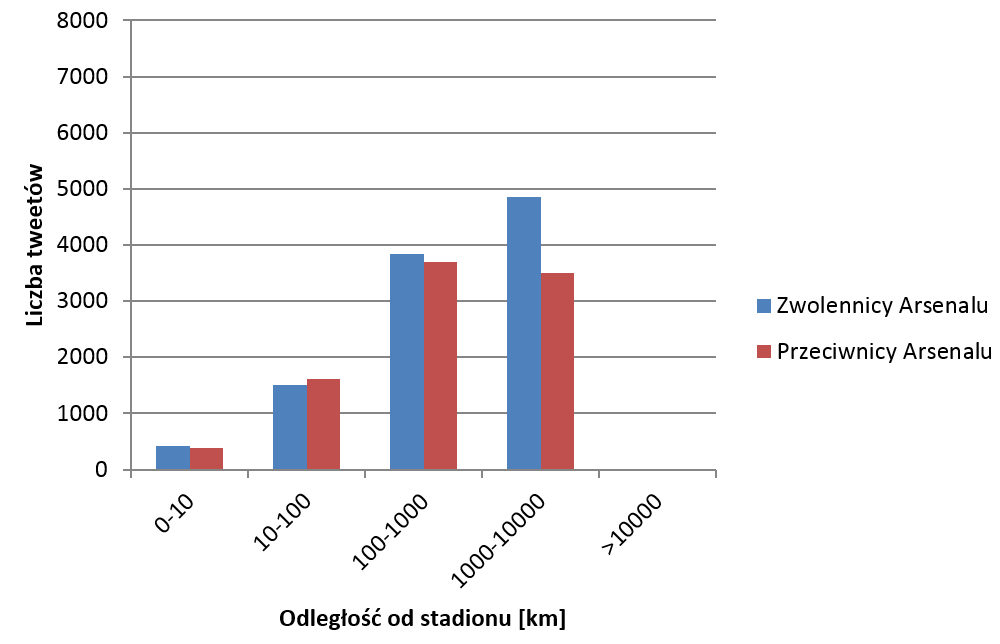
\includegraphics[width=95mm]{img/odleglosc-od-stadionu-home.PNG}
\caption{Odległość od stadionu w meczach Arsenalu u siebie}
\label{image:odleglosc-od-stadionu-gospodarz}
\end{figure}


\begin{figure}[ht!]
\centering
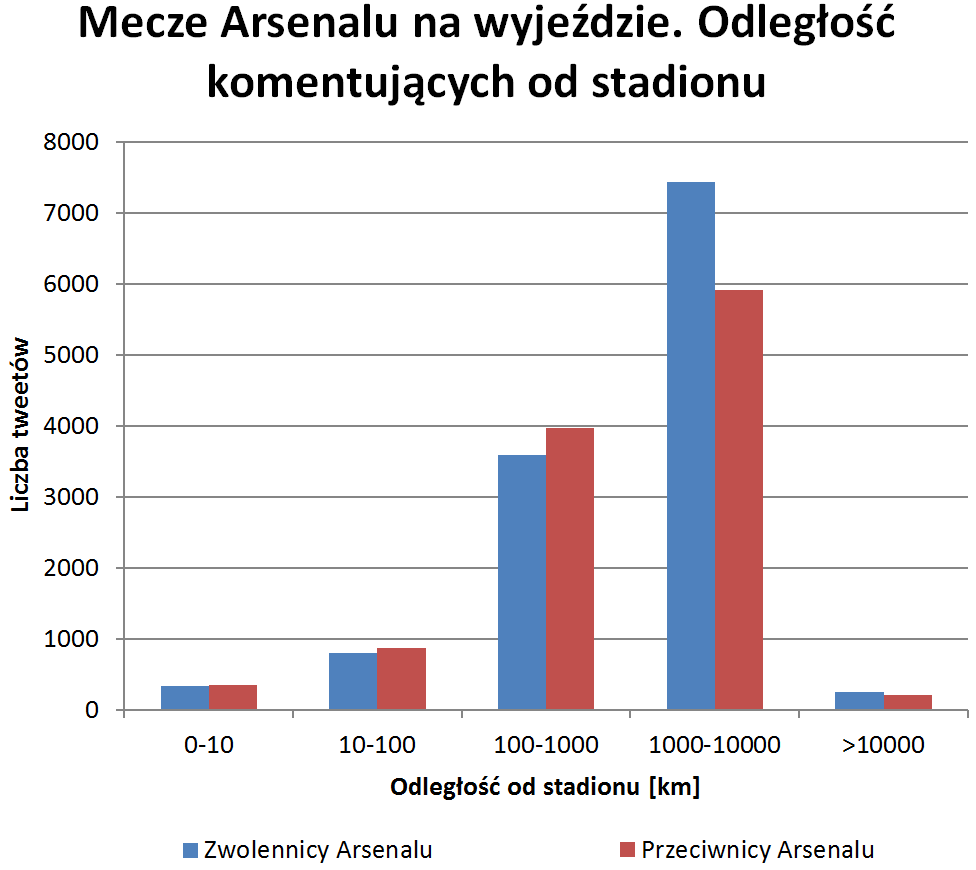
\includegraphics[width=95mm]{img//odleglosc-od-stadionu-away.png}
\caption{Odległość od stadionu w meczach Arsenalu na wyjeździe}
\label{image:odleglosc-od-stadionu-gosc}
\end{figure}

To co możemy na nich zaobserwować to fakt, że gdy Arsenal rozgrywa spotkanie na
własnym stadionie \refimg{image:odleglosc-od-stadionu-gospodarz}, wówczas liczba
wpisów zwolenników przeważa wpisy przeciwników.
Zwłaszcza w odległości 0-10 i 10-100 kilometrów od stadionu.
Gdy natomiast mecz odbywa się na wyjeździe
\refimg{image:odleglosc-od-stadionu-gosc}, wówczas lekko przeważające są wpisy,
których autorami są przeciwnicy Arsenalu.
W przypadku kiedy spojrzymy na kolumnę z wpisami wysyłanymi z odległości
1000-10000 tysięcy kilometrów od stadionu wtedy w obu przypadkach więcej wpisów
wysyłanych jest przez zwolenników londyńskiego klubu.
Widać więc, że spora część kibiców Arsenalu zapewne komentuje z Londynu
i nie przemieszcza się za swoją drużyną na każdy mecz. Wówczas, gdy klub rozgrywa
spotkanie na wyjeździe bliżej stadionu są kibice drużyny przeciwnej,
którzy tworzą wpisy odznaczające się raczej niechęcią do Arsenalu. 
Jeśli natomiast
chodzi o kibiców z dalszych zakątków świata to, można stwierdzić, że
jeśli interesują się oni tą drużyną, to raczej nastawieni są do niej pozytywnie
i łatwiej jest o sympatyków niż antyfanów.


\subsection{Rozkład wpisów z geolokacją w czasie meczu}
\label{subsection:geowpisy}
Pośród wszystkich zebranych tweetów tylko 3.06\% z nich zawierało informacje o
geolokacji. Poniżej na podstawie meczu Chelsea F.C. z Southampton F.C.
(01.12.2013 r.) zaprezentowano porównanie
(rys. \ref{image:wpisy-odsetek-geotagged}) liczby wpisów z geolokacją do
wszystkich wpisów.

\begin{figure}[ht!]
\centering
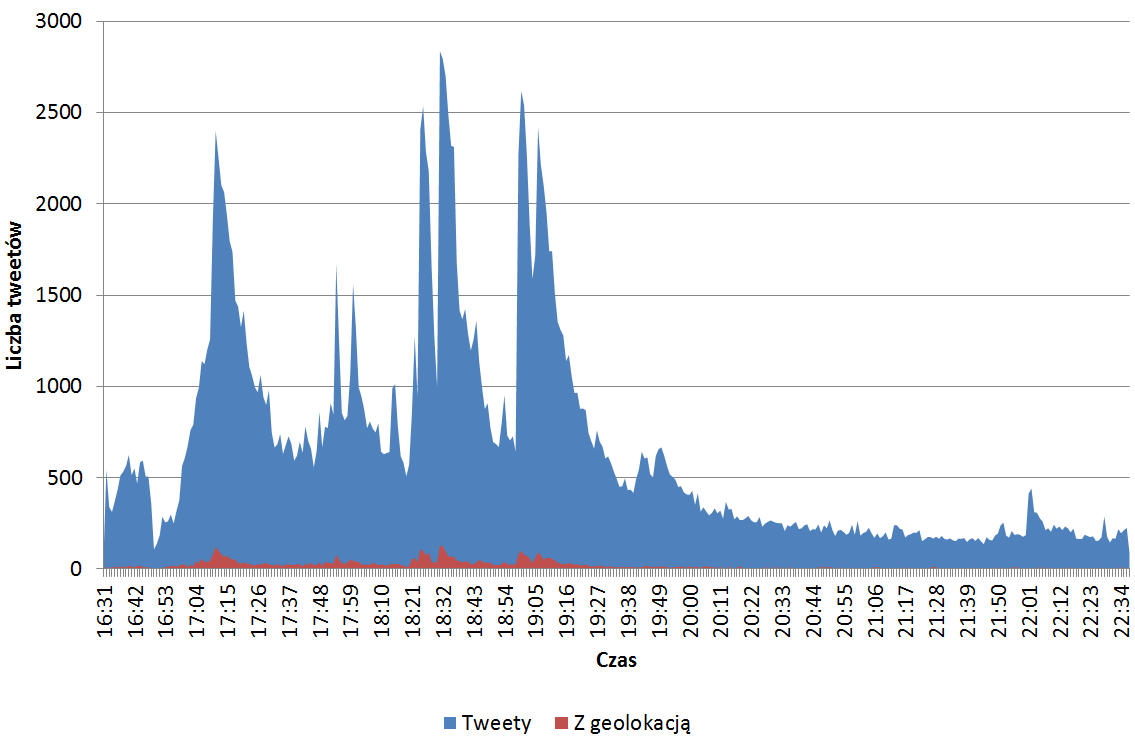
\includegraphics[width=120mm]{img/tweet-geo-w-meczu.PNG}
\caption{Rozkład wpisów z geolokacją w trakcie meczu}
\label{image:wpisy-odsetek-geotagged}
\end{figure}


Wykres jednoznacznie obrazuje o jakiej różnicy jest mowa. Nieco ponad 3\% 
wpisów z geolokacją to bardzo niewiele. Widać, że liczba takich tweetów
rośnie w tych samych momentach, gdy rośnie ogólna liczba wpisów.
Niestety (z punktu widzenia badań) geotagowanie wpisów
nie jest jeszcze czymś powszechnym i zapewne musi minąć trochę czasu,
by użytkownicy serwisów społecznościowych chętniej dzielili się miejscem,
w którym się znajdują.

\begin{comment}
\clearpage
\subsection{*Sentyment a położenie geograficzne}
Dzięki zastosowaniu georeversingu przy pomocy Open Street Map,
możliwe było odczytanie ze współrzędnych tweetów zawierających geolokalizację
szczegółów dotyczących danego miejsca.
Tym sposobem, do każdego wpisu dołączone zostały informacje o kraju,
hrabstwie/powiacie oraz mieście, z którego został on wysłany. W połączeniu z
analizą sentymentu zaprezentować można nastroje jakie pojawiają się
w różnych miejscach. Poniżej przedstawiam wykresy pokazujące wartość
sentymentu w różnych obszarach geograficznych, które zostały zaobserwowane
podczas meczu Chelsea F.C. z Liverpool F.C. (29.12.2013 r.) zakończonego
wynikiem 2-1. Są to rysunki z sentymentem w krajach \ref{image:sentyment-kraje},
powiatach/hrabstwach (ang. county) \ref{image:sentyment-hrabstwa}
oraz miastach \ref{image:sentyment-miasta}.

\begin{figure}[ht!] 
\centering
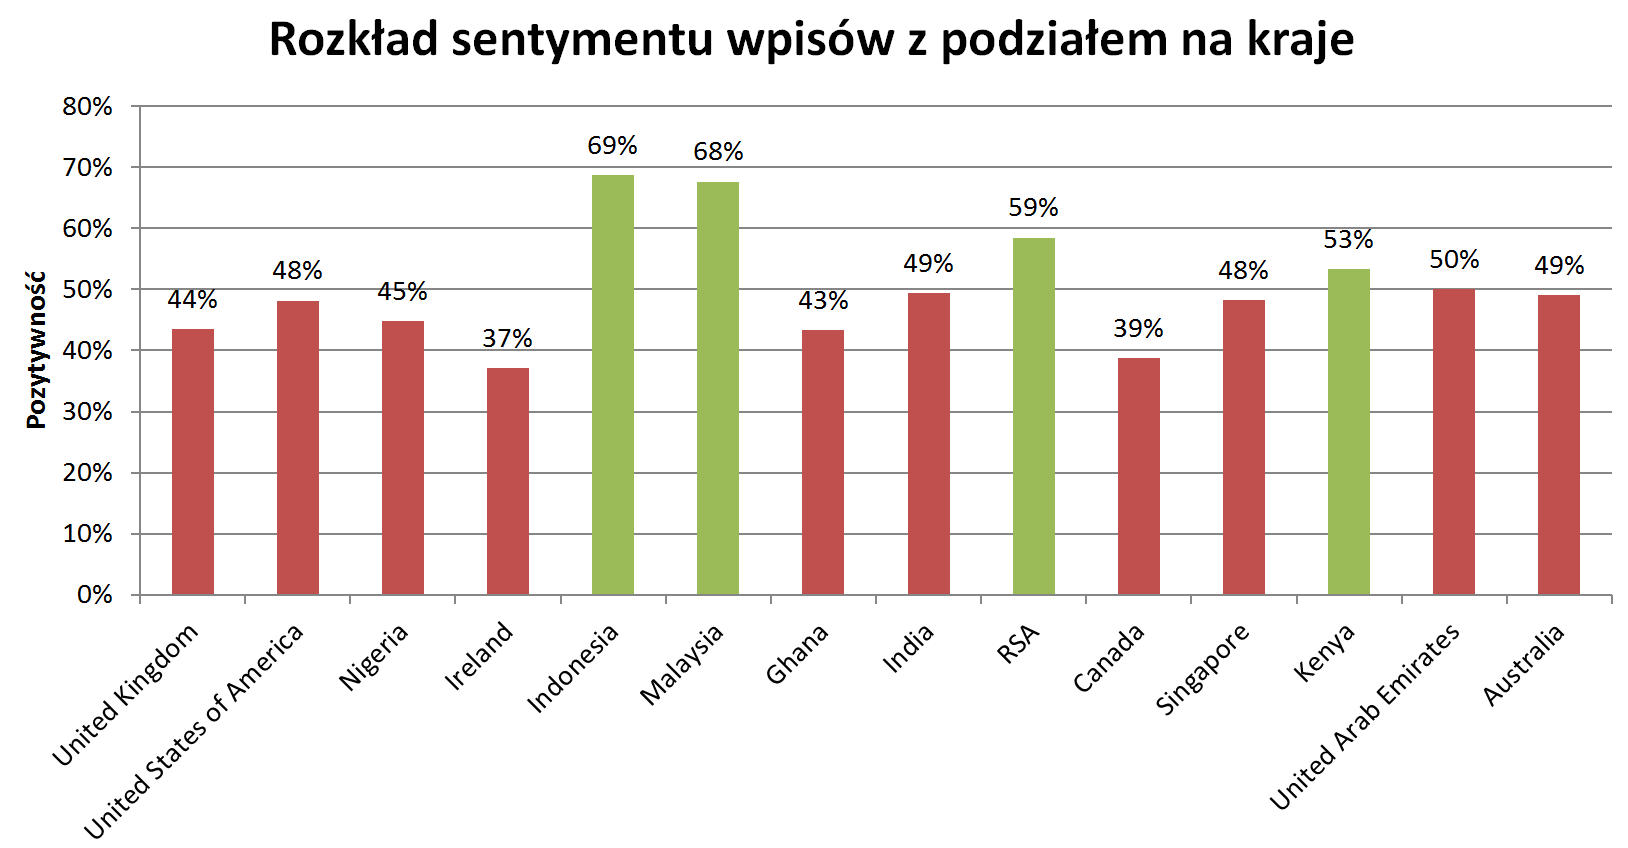
\includegraphics[width=140mm]{img/sentyment-kraje.PNG}
\caption{Sentyment wpisów z podziałem na kraje}
\label{image:sentyment-kraje}
\end{figure}

\begin{figure}[ht!]
\centering
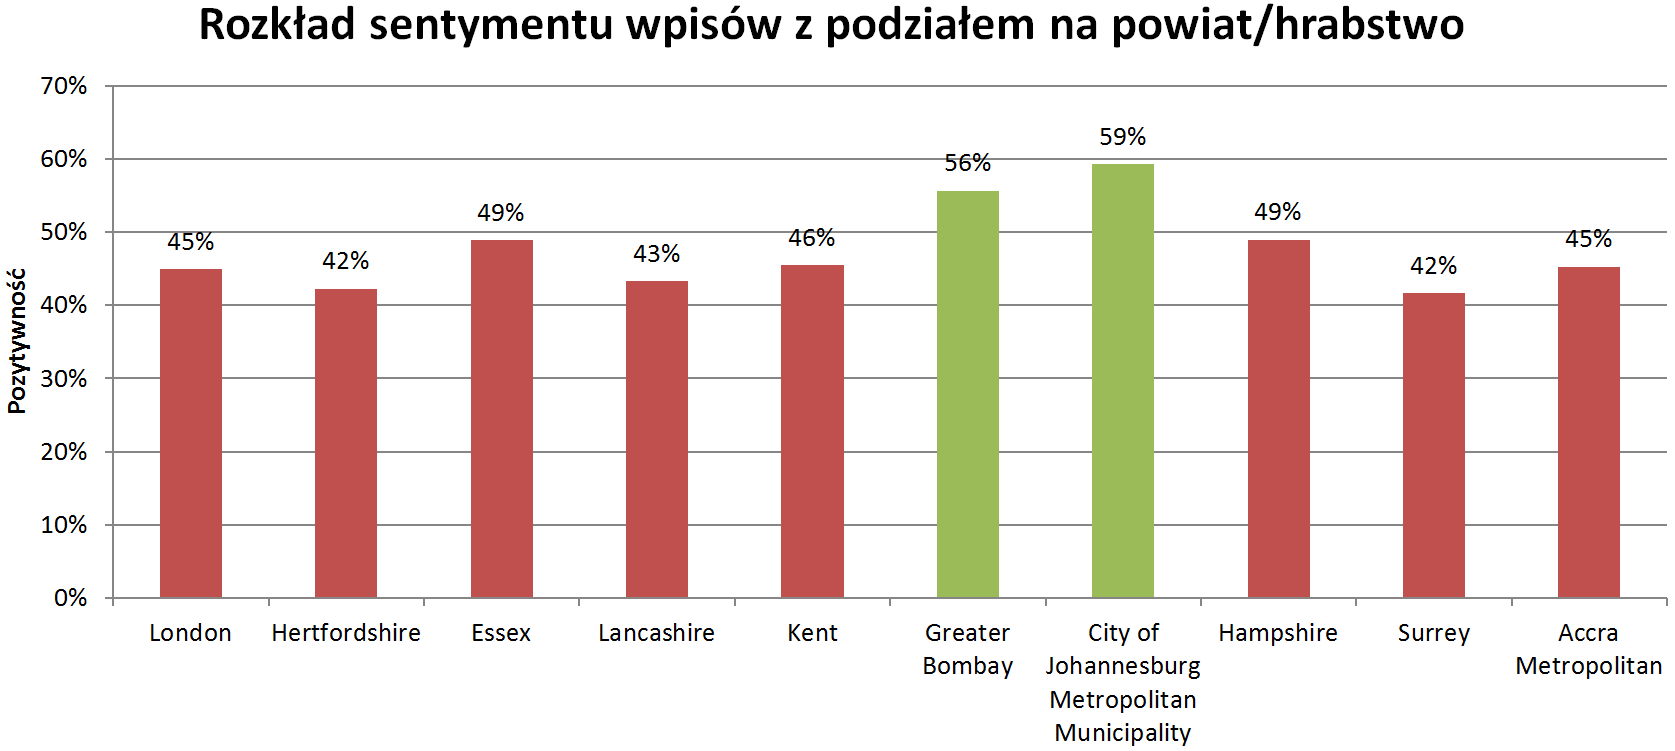
\includegraphics[width=140mm]{img/sentyment-powiaty.PNG}
\caption{Sentyment wpisów z podziałem na powiat/hrabstwo}
\label{image:sentyment-hrabstwa}
\end{figure}

\clearpage

\begin{figure}[ht!]
\centering
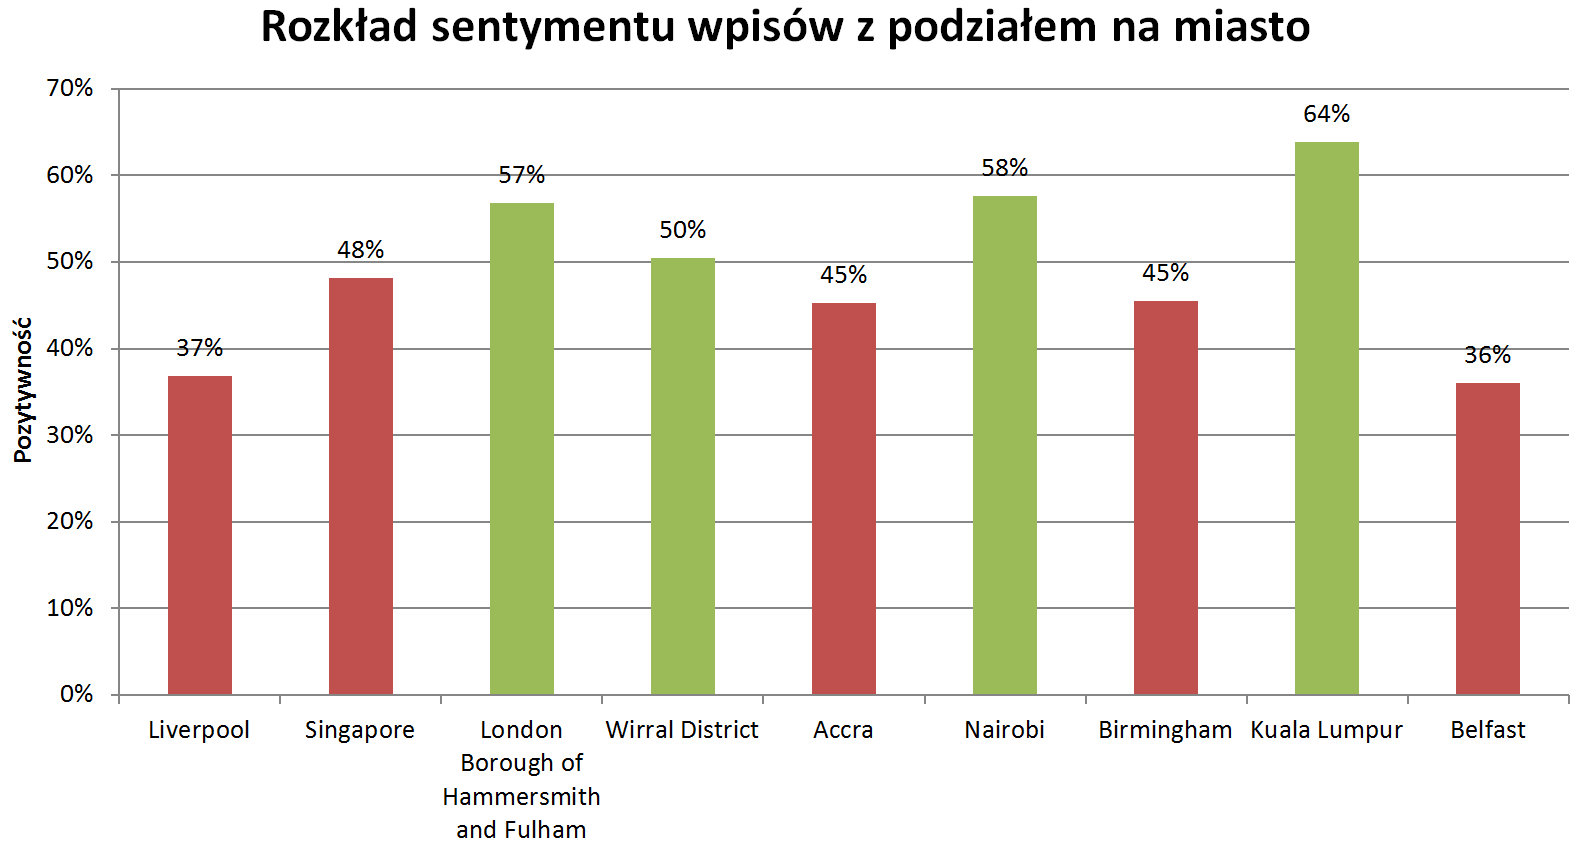
\includegraphics[width=140mm]{img/sentyment-miasto.PNG}
\caption{Sentyment wpisów z podziałem na miasta}
\label{image:sentyment-miasta}
\end{figure}

\subsubsection{Obserwacje i wnioski}
\end{comment}
















% %%%%%%%%%%%%%%%%%%%%%%%%%%%%%%%%%%%%%%%%%%%%%%%%%%%%%%%%% PODSUMOWANIE
\section{Podsumowanie eksperymentów}
Zaprezentowane powyżej eksperymenty potwierdziły, że zastosowane przeze mnie
podejście do analizy dużej sieci społecznej z wykorzystaniem analizy sentymentu
i geolokacji powiodło się. Przedstawiony w rozdziale
\ref{section:koncepcjaialgorytmanalizysentymentu} algorytm okazał się skutecznym
narzędziem pokazującym zmieniające się nastroje wśród kibiców, a także pomógł zbadać sposoby interakcji między nimi z podziałem na zwolenników i przeciwników.
Geolokacja, chociaż jeszcze niezbyt popularna, pokrywa się z tym czego można
się spodziewać.

Najwięcej wpisów pochodzi z miejsc, w których faktycznie jest zainteresowanie
danym tematem. Okazało się, że kibice najchętniej komentujące mecze z
największymi rywalami, a podobieństwo zbioru użytkowników między kolejnymi
spotkaniami jest tym większe im mniej popularny jest mecz -- potwierdzając tym
samym, że to najzagorzalsi fani są ze swoim klubem niezależnie od sytuacji.

Przeprowadzone eksperymenty udowodniły, że można wykorzystać nowoczesne techniki
komputerowe do badania dużych sieci społecznych wzbogacając je o analizę
sentymentu i geolokację, które służą do lepszego zrozumienia badanych
społeczności.



\chapter{Zakończenie i wnioski}
\section{Podsumowanie}
%%%%%%%%%%%%%%%%%%%%%%%%%%%%%%%%%%%%%%%%%%%%%%%%%%%%%%%%%%%%%%%%%%%%%%%%%%%%%%%%
%%%%  DOPISAĆ O TYM CO UDAŁO SIĘ ZROBIĆ -- DODANO NEGACJE DO ANALIZY SENTYMENTU
%%%%%%%%%%%%%%%%%%%%%%%%%%%%%%%%%%%%%%%%%%%%%%%%%%%%%%%%%%%%%%%%%%%%%%%%%%%%%%%%

W niniejszej pracy próbowano powiązać ze sobą analizę sentymentu i dane
geolokacyjne w celu wzbogacenia analizy użytkowników sieci społecznościowych.
Cel można uznać za osiągnięty.

Analiza sieci społecznych pozwala pokazać w jaki sposób osoby badane łączą się
ze sobą i jaka jest charakterystyka tych połączeń. Pokazuje wielkość
utworzonych grup i ich trwałość.

Zastosowanie analizy sentymentu dostarcza informacje, dzięki którym
możemy odkrywać przyczyny tworzenia się takich a nie innych grup
a także pomaga dowiedzieć się, dlaczego między różnymi grupami występują
konkretne rodzaje relacji. Korzystając z tej dziedziny nauki możemy także
skorelować nastroje społeczne z wydarzeniami na świecie. W niektórych przypadkach
zauważony sentyment może być w miarę przewidywalny -- tak jak w badaniu 
kibiców piłkarskich, gdzie związany jest z wynikiem meczu -- ale w innych
może pozwalać odkrywać niezauważane do tej pory ciągi przyczynowo-skutkowe.

Analiza sieci społecznych może również prowadzić do bogatszych wniosków
poprzez zastosowanie danych związanych z geolokalizacją. Powiązanie informacji
o fizycznym położeniu użytkowników, a także o sentymencie jaki generują
daje dodatkowy obraz pozwalający zrozumieć połączenia między nimi.

Dodatkowo w tej pracy udało się wykorzystać dane pochodzące z serwisu 
społecznościowego -- którym był Twitter.
Jest to bardzo ciekawe medium, które może być szeroko używane do automatycznego
badania nastrojów i sieci społecznych. Pokazano w jaki sposób takie dane
uzyskać, przetworzyć i wykorzystać do podobnych badań. Zaprezentowane zostało podejście,
dzięki któremu badanie dużych grup ludzi można przeprowadzić bez ich wiedzy
i w sposób automatyczny. Dzięki temu uzyskuje się bardziej wiarygodne wyniki.
Użytkownicy nie wiedzą, że są obserwowani i zachowują się w sposób naturalny.


\section{Wpływ pracy na otaczający świat}
Praca ta prezentuje w jaki sposób można połączyć ze sobą analizę sieci społecznych,
analizę sentymentu i analizę geolokalizacji. Udowadnia, że badanie nastrojów
w społeczeństwie można zautomatyzować aplikując komputerowe techniki przetwarzania
dużych zbiorów danych. Pokazuje, że zastosowanie analizy sentymentu i geolokacji
może istotnie wzbogacić analizę dużych grup ludzi.

Zastosowanie automatycznych technik badania dużych sieci społecznych
może uprościć sposoby komunikacji z takimi grupami i odpowiadania na ich potrzeby.
Możemy wyobrazić sobie sytuację, w której rządy, organizacje czy firmy badając
sieci społeczne wraz z analizą i geolokacją błyskawicznie reagują na aktualne
wydarzenia. Przykładem zastosowania takich badań może być prezentowanie
spersonalizowanych reklam. Gdy na przykład dana drużyna przegrywa, jej kibicom
można by wyświetlać po zakończonym meczu inny zestaw reklam niż kibicom drużyny 
przeciwnej. Firmy oferujące swoje usługi czy produkty na całym świecie
mogą szybko reagować na opinie czy błędy zgłaszane przez sfrustrowanych internautów
w serwisach społecznościowych poprawiając swój wizerunek i pokazując dbałość
o klienta. Rządy czy partie polityczne mogą wykorzystać sieci społeczne,
sentyment i geolokacje do odpowiednich zmian, ustaw dotyczących konkretnych grup
społecznych, aby polepszyć wśród nich swoje notowania.

Praca pokazuje, że wykorzystanie mediów internetowych, czy
serwisów społecznościowych może dać wymierne korzyści. Potwierdza, że
świat wirtualny i realny przenikają się. Tak samo reagujemy na różne
wydarzenia niezależnie od tego, czy dzielimy się swoimi opiniami z bliskimi będącymi obok
nas czy z całym światem korzystając z serwisów społecznościowych. Jeśli więc
zarządy firm lub organizacji nie wierzą lub wahają się nad sensem przeprowadzenia
takich badań, to niniejsza praca może być dla nich dowodem, że warto bliżej
przyjrzeć się zaprezentowanym tutaj aspektom. Może być więc punktem wyjścia
do prowadzenia własnych badań na interesujące dany podmiot tematy.



\section{Możliwe kierunki rozwoju}
% plan dalszego rozwoju systemu
% w pływ pracy, zastosowanie wyników teraz i w przyszłości

Zaprezentowana praca jest ukierunkowana na wąską dziedzinę -- bada zachowania
kibiców piłkarskich. W związku z tym, aby rozszerzyć jej zakres konieczne
jest przeprowadzenie kilku działań celem jej rozwoju. Kilka możliwych kierunków to:

\subsubsection{Rozszerzenie o inne języki naturalne}
Zastosowany mechanizm analizy sentymentu jest skupiony jedynie na
języku angielskim. Aby móc badać większe grupy ludzi koniecznym jest opracowanie
techniki badającej również inne języki. Oczywiście w pewnym stopniu można 
wykorzystać podejście zastosowane w tej pracy, należy jednak mieć na uwadze
różnice między budową używanych języków. Zupełnie inne konstrukcje językowe
są w języku angielskim a zupełnie inne na przykład w języku polskim.
Oczywiste jest więc, że nie można w taki sam sposób podejść do badania
wpisów w różnych językach. Rozbudowanie mechanizmu o kolejne języki pozwoliłoby
uzyskać bogatsze wyniki.

\subsubsection{Odkrywanie tematów rozmów}
Ciekawym rozszerzeniem badania sieci społecznych w kontekście przetwarzania
języka naturalnego byłoby opracowanie i zastosowanie metody pozwalającej
odkrywać tematy rozmów użytkowników. W zaprezentowanym podejściu badany jest
jedynie sentyment wpisów, nie ma natomiast informacji na temat tego o czym dokładnie
dyskutują użytkownicy Twittera. Użycie mechanizmu ekstrakcji tematów rozmów
z wpisów z pewnością wzbogaciłoby analizę sieci społecznych.


\subsubsection{Wzbogacenie techniki badania sentymentu}
Badanie wydźwięku wypowiedzi zostało zautomatyzowane. Wykorzystuje do tego celu
wpisy tworzone przez badaną grupę. Interesującym rozszerzeniem techniki badania 
sentymentu mogłoby być zastosowanie ręcznie stworzonego słownika.
Mógłby on nieco skorygować niektóre wyniki analizy wydźwięku wypowiedzi i
polepszyć ich jakość. Dodatkowo pozwoliłoby to na zastosowanie metody analizy sentymentu
w szerszej dziedzinie badań. Aktualna metoda jest w pewien sposób zorientowana
na środowisko piłkarskie i niekoniecznie dawałaby dobre rezultaty w innym
zbiorze danych -- na przykład wpisach politycznych. Skorzystanie ze słownika
i zwięszkenie zakresu badanych wpisów pozwoliłoby szerzej zastosować
opracowaną metodę.

\subsubsection{Bliższe przyjrzenie się grupom}
Dodatkowym kierunkiem rozwoju mogło by być bliższe przyjrzenie się grupom,
które się utworzyły. Można by na przykład skierować swoje badania
na szukanie liderów tych grup, przyczyn ich pojawiania się i sposobów w jaki
oddziałują na resztę grupy w zależności od sentymentu jaki sami generują,
jaki generują dane grupy czy w jakiej lokalizacji geograficznej się znajdują. 






	
\bibliographystyle{plain}
\bibliography{bibliografia}
%---------------------------------------------------------------------------
\end{document}
